%definira klasu dokumenta 
\documentclass[12pt]{report} 

%prostor izmedu naredbi \documentclass i \begin{document} se zove uvod. U njemu se nalaze naredbe koje se odnose na cijeli dokument

%osnovni LaTex ne može riješiti sve probleme, pa se koriste različiti paketi koji olakšavaju izradu željenog dokumenta
\usepackage[croatian]{babel} 
\usepackage{amssymb}
\usepackage{amsmath}
\usepackage{txfonts}
\usepackage{mathdots}
\usepackage{titlesec}
\usepackage{array}
\usepackage{lastpage}
\usepackage{etoolbox}
\usepackage{longtable, tabu}
\usepackage{color, colortbl}
\usepackage{adjustbox}
\usepackage{geometry}
\usepackage[classicReIm]{kpfonts}
\usepackage{hyperref}
\usepackage{fancyhdr}

\usepackage{float}
\usepackage{setspace}
\restylefloat{table}
\usepackage{enumitem}


\patchcmd{\chapter}{\thispagestyle{plain}}{\thispagestyle{fancy}}{}{} %redefiniranje stila stranice u paketu fancyhdr

%oblik naslova poglavlja
\titleformat{\chapter}{\normalfont\huge\bfseries}{\thechapter.}{20pt}{\Huge}
\titlespacing{\chapter}{0pt}{0pt}{40pt}


\linespread{1.3} %razmak između redaka

\geometry{a4paper, left=1in, top=1in,}  %oblik stranice

\hypersetup{ colorlinks, citecolor=black, filecolor=black, linkcolor=black,	urlcolor=black }   %izgled poveznice


%prored smanjen između redaka u nabrajanjima i popisima
\newenvironment{packed_enum}{
	\begin{enumerate}
		\setlength{\itemsep}{0pt}
		\setlength{\parskip}{0pt}
		\setlength{\parsep}{0pt}
	}{\end{enumerate}}

\newenvironment{packed_item}{
	\begin{itemize}
		\setlength{\itemsep}{0pt}
		\setlength{\parskip}{0pt}
		\setlength{\parsep}{0pt}
	}{\end{itemize}}


%boja za privatni i udaljeni kljuc u tablicama
\definecolor{LightBlue}{rgb}{0.9,0.9,1}
\definecolor{LightGreen}{rgb}{0.9,1,0.9}


%podesavanje zaglavlja i podnožja

\pagestyle{fancy}
\lhead{Programsko inženjerstvo}
\rhead{Planinarski dnevnik}
\lfoot{RuntimeTerror}
\cfoot{stranica \thepage/\pageref{LastPage}}
\rfoot{\today}
\renewcommand{\headrulewidth}{0.2pt}
\renewcommand{\footrulewidth}{0.2pt}


\begin{document} 
	
	
	
	\begin{titlepage}
		\begin{center}
			\vspace*{\stretch{1.0}} %u kombinaciji s ostalim \vspace naredbama definira razmak između redaka teksta
			\LARGE Programsko inženjerstvo\\
			\large Ak. god. 2020./2021.\\
			
			\vspace*{\stretch{3.0}}
			
			\huge{Planinarski Dnevnik}\\
			\Large Dokumentacija, Rev. \textit{$1.0$}\\
			
			\vspace*{\stretch{12.0}}
			\normalsize
			Grupa: \textit{$RuntimeTerror$}\\
			Voditelj: \textit{Ivan Martinović}\\
			
			
			\vspace*{\stretch{1.0}}
			Datum predaje: \textit{13.11.2020.}\\
	
			\vspace*{\stretch{4.0}}
			
			Nastavnik: \textit{Katarina Labor}\\
		
		\end{center}

	
	\end{titlepage}

	
	\tableofcontents

	\chapter{Dnevnik promjena dokumentacije}
		
		%\textbf{\textit{Kontinuirano osvježavanje}}\\
				
		
		\begin{longtabu} to \textwidth {|X[2, l]|X[13, l]|X[3, l]|X[3, l]|}
			\hline \multicolumn{1}{|l|}{\textbf{Rev.}}	& \multicolumn{1}{l|}{\textbf{Opis promjene/dodatka}} & \multicolumn{1}{|l|}{\textbf{Autori}} & \multicolumn{1}{l|}{\textbf{Datum}} \\[3pt] \hline
			\endfirsthead
			
			\hline \multicolumn{1}{|l|}{\textbf{Rev.}}	& \multicolumn{1}{l|}{\textbf{Opis promjene/dodatka}} & \multicolumn{1}{|l|}{\textbf{Autori}} & \multicolumn{1}{l|}{\textbf{Datum}} \\[3pt] \hline
			\endhead
			
			\hline 
			\endlastfoot
			
			0.1 & Napravljen predložak.	& I.M & 14.10.2020. 		\\[3pt] \hline 
			0.2	& Dodan opis projektnog zadatka & J.K, H.L, N.K, I.M, D.K & 14.10.2020. 	\\[3pt] \hline 
			0.3 & Dodana osnovna verzija funkcionalnih zahtjeva & J.K, I.M, M.R & 14.10.2020. \\[3pt] \hline 
			0.3.1 & Ispravljeni funkcionalni zahtjevi & I.M & 17.10.2020 \\[3pt] \hline 
			0.4 & Dodana početna verzija obrazaca uporabe & D.K, N.K & 19.10.2020 \\[3pt] \hline 
			0.4.1 & Ispravljeni, povezani i dodani novi scenariji obrazaca uporabe  & I.M & 21.10.2020. \\[3pt] \hline 
			0.4.2 & Izmijenjeni i dodani novi obrasci uporabe & I.M & 25.10.2020 \\[3pt] \hline 
			0.5 & Dodani dijagrami obrazaca uporabe & I.M & 25.10.2020 \\[3pt] \hline 
			0.6 & Dodani sekvencijski dijagrami & J.K, H.L, I.M & 29.10.2020 \\[3pt] \hline 
			0.7 & Dodan opis baze podataka zajedno s tablicama & M.R, I.M & 05.11.2020 \\[3pt] \hline 
			0.7.1 & Dodani nefunkcionalni zahtjevi te zahtjevi domene primjene & D.K, N.K & 05.11.2020 \\[3pt] \hline 
			0.8 & Dodan opis arhitekture sustava & J.K & 5.11.2020 \\[3pt] \hline 
			0.8.1 & Ažuriran opis baze podataka, preimenovane tablice i dorađeni atributi & I.M & 10.11.2020 \\[3pt] \hline
			0.8.2 & Zamijenjen dijagram baze podataka & M.R & 10.11.2020 \\[3pt] \hline
			0.8.3 & Ispravljeni opisi i dijagrama, ispravljene gramatičke pogreške i uklonjeni dijelovi dokumentacije nevažni za prvu predaju & I.M & 11.11.2020 \\[3pt] \hline
			0.9 & Dodani dijagrami razreda te opisi dijagrama razreda & I.M & 11.11.2020 \\[3pt] \hline 
			1.0 & Završna verzija dokumentacije - prva predaja & I.M & 13.11.2020 \\[3pt] \hline
			%1.3 & Popravljeni dijagrami obrazaca uporabe & Jović & 15.09.2013. \\[3pt] \hline 
			%1.5 & Generalna revizija strukture dokumenta & Ivošević & 19.09.2013. \\[3pt] \hline 
			%1.5.1 & Manja revizija (dijagram razmještaja) & Jović & 20.09.2013. \\[3pt] \hline 
			%\textbf{2.0} & Konačni tekst predloška dokumentacije  & Ivošević & 28.09.2013. \\[3pt] \hline 
			%&  &  & \\[3pt] \hline
			
			
		\end{longtabu}
	
	\chapter{Opis projektnog zadatka}
		
		%\textbf{\textit{dio 1. revizije}}\\
		
		U današnje vrijeme većina ljudi živi užurbanim tempom, stoga svaki slobodan trenutak žele iskoristiti za odmor i rekreaciju. Mnoge ljude privlači boravak na svježem zraku te kao rezultat toga, sve više ljudi izabire planinarenje kao jednu od brojnih mogućnosti koje im se nude. Međutim, planinari pri odabiru rute za svoje planinarske izlete često nemaju dovoljno informacija pa se koriste usmenom predajom i nagađanjima. Tako planinari, osobito planinari rekreativci, nailaze na različite probleme od kojih su najčešći krive informacije o stazama i rutama ili planinarski domovi bez odgovarajuće infrastrukture. Upravo zbog toga pokrenut je projekt čiji je cilj razvoj i evolucija programskog proizvoda, odnosno web aplikacije „Planinarski dnevnik“. Aplikacija će uvelike pomoći planinarima u organiziranju svojih planinarskih izleta, ali i ponuditi točne informacije o rutama na pojedinim izletima te povezati planinare poznanike u vlastitu planinarsku zajednicu. Osim toga, planinari će moći pretraživati i planinarske domove koji se nalaze na odabranim stazama, a za svaki dom će biti prikazane koje pogodnosti on nudi (prenoćište, topao obrok, pitka voda, struja, grijanje itd.). \\
		
		Opseg projektnog zadatka sadrži sve aktivnosti i zadatke koji su vezani uz izradu aplikacije. Za početak se radi analiza aplikacije kako bi se utvrdilo koliko će okvirno vremena biti potrebno za izradu određene komponente aplikacije. U tome dobrim dijelom pomažu dnevnik sastajanja i dnevnik aktivnosti koji služe kao kontrolne točke pomoću kojih se vidi ide li daljnji napredak aplikacije u dobrom smjeru. Na tim sastancima prisutni su asistenti koji su stručnjaci za ovo područje i svojim savjetima višestruko pomažu timu. \\
		
		Za izradu „Planinarskog dnevnika“ predviđen je vremenski period od 13 tjedana, odnosno jednog fakultetskog semestra. Radi se analiza interesnih sudionika s namjerom da se što točnije odredi broj korisnika koji će biti zainteresirani za korištenje aplikacije. Svrha same aplikacije je educirati studente na fakultetu pa shodno tome ne postoje troškovi prilikom izrade iste. Krajnji cilj je potpuno razvijena aplikacija s ispravnom programskom potporom koja sadrži sve zahtijevane komponente i podržava rad više korisnika u stvarnom vremenu. Kada je navedeno postignuto, aplikacija je spremna za lansiranje na tržište kako bi se korisnici mogli njome služiti.\\
		
		Aplikacija „Planinarski dnevnik“ zasigurno će biti najzanimljivija planinarima kojima je i namijenjena, ali također i mnogobrojnim ustanovama poput planinarskih domova kojima će omogućiti promociju u širem krugu korisnika. Potencijalno bi moglo doći do povećanja prihoda kao rezultat brojnih usluga koje planinarski domovi pružaju, ali i poboljšanja kvalitete istih sukladno s porastom broja planinara koji ih posjećuju. Proširit će se opseg planinarskog turizma na manje poznata područja tako što će postati vidljiva širem krugu korisnika aplikacije. Također, korisnost ove aplikacije odrazit će se na HGSS (Hrvatska gorska služba spašavanja) koja će efikasnije saznati sve potrebne informacije o kretanju i ruti planinara u slučaju nesreće ili nestanka. Evidentno je da će se područje pretrage znatno smanjiti jer će planinar unaprijed odrediti rutu svojeg kretanja.\\
		
		Pokretanjem aplikacije svakom korisniku prvotno će biti dodijeljena uloga \underbar{Gost} koja omogućava pretraživanje postojećih planinarskih domova prema dostupnoj infrastrukturi (pitka voda, hrana, prenoćište...) ili
		pretraživanje planinarskih staza prema zahtjevnosti, trajanju ili duljini. Za sve daljnje aktivnosti korisnik će se morati registrirati u sustav tako što će u predloženu formu za registraciju unijeti osobne podatke:
		\begin{packed_item}
			\item ime
			\item prezime
			\item e-mail
			\item lozinku
			\item sliku (opcionalno)
			\item nešto više o sebi (opcionalno)
			\item datum rođenja (opcionalno)
			\item mjesto stanovanja (opcionalno)	
		\end{packed_item}
	 
		Nakon što se korisnik registrira dodijelit će mu se uloga \underbar{Planinar} i moći će pristupiti vlastitom profilu. Omogućit će mu se pregled i uređivanje osobnih podataka te u krajnjem slučaju uklanjanje korisničkog računa. Planinar može uspostaviti odnos s ostalim registriranim planinarima tako što šalje zahtjeve za "prijateljstvom", odnosno zahtjeve za dodavanje na popis vlastite planinarske zajednice, ali i na način da ostale članove svoje planinarske zajednice pozove na određeni događaj. Prema unaprijed određenom predlošku dopušta se stvaranje vlastitih planinarskih staza kao i vlastitih događaja. Uz to se nudi i mogućnost ocjenjivanja stvorenih planinarskih staza kao i prijava netočnih ili nepreciznih informacija vezanih uz pojedine staze, što može biti od velike koristi svim planinarima, osobito početnicima koji na osnovu najviše ocjene mogu odabrati svoju željenu stazu. Na naslovnici će biti prikazane objave prijatelja planinara, a na zidu obavijesti će biti vidljiv popis prihvaćenih ili odbijenih pozivnica te prihvaćenih ili odbijenih zahtjeva za prijateljstvom. Nudi se i svrstavanje planinarske staze ili doma na popis željenih te dodavanje ranije odrađenih planinarskih staza u osobnu arhivu. Dolaskom planinara na cilj evidentirat će se njihovo prisutstvo, a nakon određenog broja osvojenih vrhova ostvarit će pravo na bedž kao jednu vrstu motivacije za još veću aktivnost u budućnosti. \\
		
		Svaki planinar ima priliku dobiti ulogu \underbar{Dežurnog planinara} tako što tu ulogu zatraži od administratora. Nakon što bilo koji registrirani planinar posjeti određeni planinarski dom, dobiva potvrdu o posjetu od planinara koji je zadužen za taj planinarski dom, tzv. dežurnog planinara.\\
		
		Sustav nadgleda \underbar{Administrator} koji ima najveće ovlasti. Ukoliko neki korisnik (planinar) ne poštuje pravila ponašanja, administrator ima pravo obrisati njegov korisnički račun. On će zaprimati primjedbe od korisnika na određene staze te će ovisno o količini netočnih informacija odlučiti hoće li staza biti izmijenjena ili uklonjena s liste. Također će odobravati zahtjeve za dežurnog planinara i dodijeliti ga određenom planinarskom domu. Time se sprječava ponavljanje istih pogrešaka u budućnosti i aplikacija će biti sve točnija i vjerodostojnija. 
		
		
		\section{Primjeri sličnih rješenja}
		Slične implementacije rješenja projektnog zadatka već postoje. Na području Republike Hrvatske možemo izdvojiti iduće: 
		\begin{packed_enum}
			\item Kao prvi primjer navodimo aplikaciju \textbf{eHPS} koja je razvijena pod pokroviteljstvom Hrvatskog planinarskog saveza. Njena svrha je omogućavanje korisniku efikasno pretraživanje podataka o svim planinarskim domovima, kućama i skloništima koji postoje na području Republike Hrvatske. Također pruža uslugu iščitavanja i proučavanja podataka o svim kontrolnim točkama i dosad otvorenim planinarskim obilaznicama.
			\item Druga slična aplikacija je \textbf{infoHPS} koja pruža uslugu pretraživanja postojećih planinarskih udruga koje su članice Hrvatskog planinarskog saveza. Za svaku traženu udrugu omogućuje prikaz informacija bitnih za korisnika poput naziva, OIB-a udruge, email-a itd. 
		\end{packed_enum}
	
			\begin{figure}[H]
			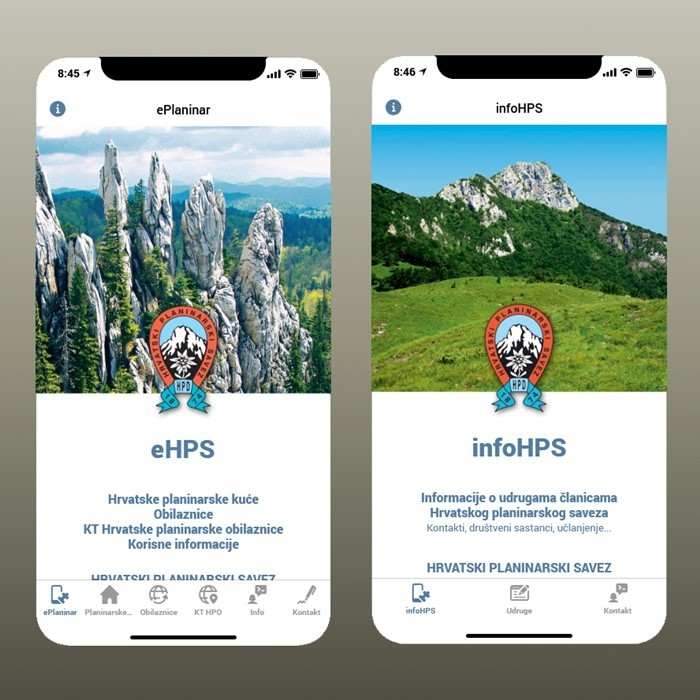
\includegraphics[scale=0.5]{slike/HPS.jpg} %veličina slike u odnosu na originalnu datoteku i pozicija slike
			\centering
			\caption{Primjeri sličnih aplikacija - eHPS i infoHPS}
			\label{fig:slične aplikacije}
			\end{figure}
	
		Na području SAD-a aplikacija \textbf{Mountain project} nudi korisnicima pretraživanje postojećih planinarskih ruta, čitanje novosti i razmjenjivanje poruka između prijavljenih korisnika.
			
			\begin{figure}[H]
				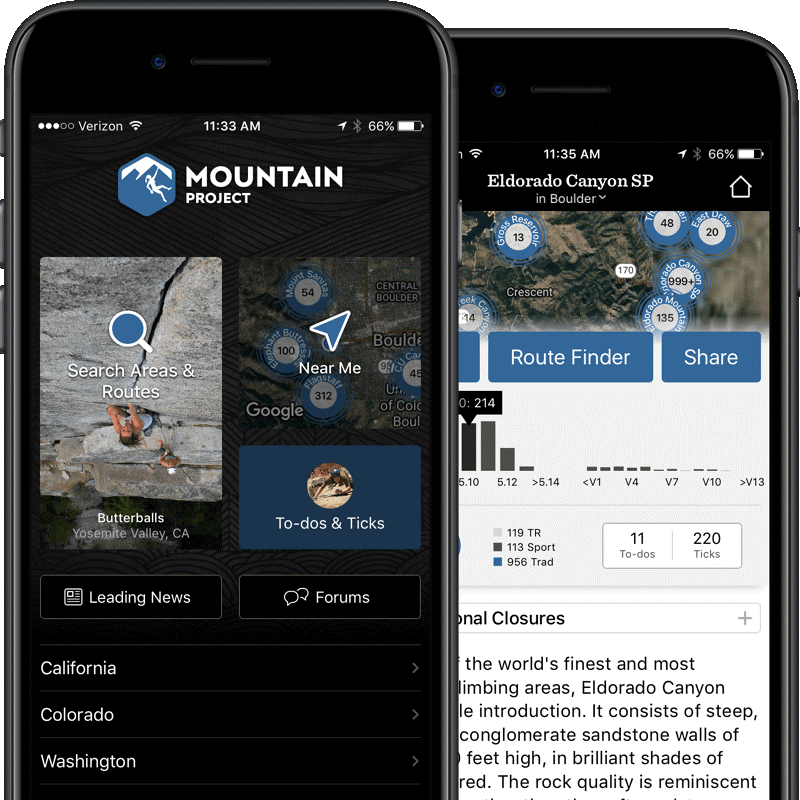
\includegraphics[scale=0.3]{slike/mountainproject.png} %veličina slike u odnosu na originalnu datoteku i pozicija slike
				\centering
				\caption{Primjer slične aplikacije - Mountain Project}
				\label{fig:slične aplikacije}
			\end{figure}
		
		\section{Moguće nadogradnje projektnog zadatka}
		Postoje brojne funkcionalnosti kojima bi se mogla nadograditi i proširiti postojeća aplikacija te ispraviti eventualne nepravilnosti. Jedna od mogućnosti je implementacija „Chat-a“ za razmjenu poruka i iskustava među planinarima koji pripadaju istoj planinarskoj zajednici. Uz to, mogao bi se dodati i neformalni forum gdje bi svi planinari mogli podijeliti svoja iskustva, doživljaje i preporuke ostatku planinarske zajednice. Aplikacija bi trebala imati i mogućnost instaliranja na pametne satove koji su postali neizostavni dio planinarske i sportske opreme.  Također bi bilo korisno kad bi korisnici odlaskom na naslovnu stranu aplikacije mogli vidjeti aktualne novosti, događanja iz planinarskog svijeta te preporučene izlete u skladu s vremenskim uvjetima. Svaki planinar mora imati odgovarajuću opremu prije nego što krene na izlet pa bi oglašavanje i prodaja planinarske opreme bio izvrstan dodatak aplikaciji. Registrirani planinar bi mogao postaviti oglas sa slikom i opisom opreme koju prodaje, cijenom i lokacijom na kojoj se nalazi. Sadašnja verzija aplikacije sadrži unesene izlete namijenjene većinom za pješačke rute. U budućnosti bi se aplikacija mogla proširiti dodavanjem ruta za bicikliranje ili čak i skijanje. Još jedna od korisnih funkcionalnosti bila bi uvođenje uloge „planinarski dom“. Uloga bi planinarskim domovima omogućila kreiranje vlastitih događaja kao što su organizirani izleti, zabave i slično. 
		
		\eject
		
	
	\chapter{Specifikacija programske potpore}
		
	\section{Funkcionalni zahtjevi}
			
			
			\noindent \textbf{Dionici:}
			
			\begin{packed_enum}
				
				\item Naručitelj (FER)
				\item Razvojni tim
				\item Administrator				
				\item Planinari (korisnici aplikacije)
				\item Zaposlenici planinarskih domova
				
			\end{packed_enum}
			
			\noindent \textbf{Aktori i njihovi funkcionalni zahtjevi:}
			
			
			\begin{packed_enum}
				\item  \underbar{Neregistrirani/neprijavljeni korisnik (inicijator) može:}
				
				\begin{packed_enum}
					
					\item pregledati popis planinarskih staza
					\item pretraživati planinarske staze
					\begin{packed_enum}
						
						\item  prema zemljopisnom položaju 
						\item  prema prosječnom trajanju pješačenja za određenu stazu
						\item  prema zahtjevnosti planinarske staze
				
					\end{packed_enum}
					\item pregledati popis planinarskih domova
					\item pretraživati planinarske domove
					\begin{packed_enum}
						\item prema dostupnoj infrastrukturi (voda, prenoćište, struja, hrana, internet)
						\item prema zemljopisnom položaju
					\end{packed_enum}
					\item se registrirati u sustav kao planinar tako što popuni formu za registraciju
				\end{packed_enum}
			
				\item  \underbar{Planinar (inicijator) može:}
				
				\begin{packed_enum}
					\item prijaviti se u sustav kao planinar
					\item odjaviti se iz sustava
					\item upravljati vlastitim korisničkim računom
						\begin{packed_enum}
							
							\item  pregledati osobne podatke 
							\item  uređivati osobne podatke
							\item  ukloniti korisnički račun
							
						\end{packed_enum}
					\item pretraživati korisnike prema imenu i prezimenu
					\item upravljati zahtjevima za prijateljstvo
					
						\begin{packed_enum}
							\item poslati zahtjev za prijateljstvom (zahtjev za dodavanjem drugog planinara na popis vlastite planinarske zajednice)
							\item prihvatiti zahtjev za prijateljstvom
							\item pregledati pristigle zahtjeve za prijateljstvom
							\item vidjeti obavijest ako je drugi planinar prihvatio njegov zahtjev
						\end{packed_enum}
					
					\item pregledati popis planinara u vlastitoj planinarskoj zajednici
					\item upravljati vlastitim planinarskim stazama
					\begin{packed_enum}
						\item stvoriti vlastitu planinarsku stazu prema unaprijed definiranom predlošku
						\item pregledati staze koje je stvorio
						\item obrisati vlastitu planinarsku stazu ukoliko je ona privatna
					\end{packed_enum}
					\item pregledati popis željenih planinarskih staza (favoriti)
					\item dodati planinarsku stazu na popis željenih
					\item ocjenjivati stvorene planinarske staze drugih planinara
					\item prijaviti netočne i neprecizne informacije vezane uz planinarske staze
					\item stvoriti događaj vidljiv na naslovnici na koji može
						\begin{packed_enum}
							
							\item  pozvati korisnike aplikacije s popisa vlastite planinarske zajednice 
							\item  pregledati popis ljudi koji dolaze na kreirani događaj
							
						\end{packed_enum}
					\item na naslovnici vidjeti nove objave korisnika s popisa vlastite planinarske zajednice
						\begin{packed_enum}
					
							\item  kreirani događaji
							\item  ostvareni bedževi
							
						\end{packed_enum}
					\item dodati ranije odrađene planinarske staze u arhivu
					\item dodati ranije posjećene planinarske domove u arhivu (zatražiti potvrdu od dežurnog planinara da je bio u domu)
					\item obzirom na svoju aktivnost zaraditi određeni bedž koji se prikazuje na njegovom profilu
					\item kontaktirati administratora u slučaju potrebe za stvaranjem novog planinarskog doma ili promjene infrastrukture već postojećeg
				\end{packed_enum}
				
				\item  \underbar{Dežurni planinar (inicijator) može:}
				
				\begin{packed_enum}
					
					\item zatražiti ulogu dežurnog planinara u određenom planinarskom domu  
					\item upravljati zaprimljenim zahtjevima za potvrdom posjeta u planinarskim domovima za koje je odgovoran
					\begin{packed_enum}
						
						\item pregledati zahtjeve
						\item potvrditi ili odbiti zahtjev
						
					\end{packed_enum}
				\end{packed_enum}
			
				\item  \underbar{Administrator (inicijator) može:}
				
				\begin{packed_enum}
					
					\item obrisati korisničke račune
					\item upravljati zaprimljenim zahtjevima za dežurnog planinara
					\begin{packed_enum}
						
						\item pregled zahtjeva
						\item prihvaćanje i odbijanje zahtjeva
					
					\end{packed_enum}
					\item upravljati planinarskim stazama
						\begin{packed_enum}
							\item pregled prijavljenih netočnih i nepreciznih informacija vezanih uz objavljene planinarske staze
							\item uređivanje staza
							\item brisanje staza
						\end{packed_enum}	
					\item upravljati planinarskim domovima
					\begin{packed_enum}
						\item pregled prijavljenih netočnih i nepreciznih informacija vezanih uz objavljene planinarske domove
						\item uređivanje postojećih planinarskih domova
						\item stvaranje novog planinarskog doma
						\item brisanje planinarskih domova
					\end{packed_enum}
					\item pregledati poruke koje su poslali planinari
					
				\end{packed_enum}
	
				\item  \underbar{Baza podataka (sudionik):}
				
					\begin{packed_enum}
						
						\item komunicira s cjelokupnim sustavom
						\item pohranjuje sve podatke nužne za uspješno funkcioniranje sustava
						
					\end{packed_enum}
			\end{packed_enum}
			
			\eject 
			
			
				
			\subsection{Obrasci uporabe}
								
				\subsubsection{Opis obrazaca uporabe}
				
					

				
				\noindent \underbar{\textbf{UC$ $1$ $ -$ $Registracija$ $}}
			\begin{packed_item}
				
				\item \textbf{Glavni sudionik: }$ $Neregistrirani korisnik aplikacije (posjetitelj)$ $
				\item  \textbf{Cilj:} $ $Stvaranje novog korisničkog računa s ulogom "planinar"$ $
				\item  \textbf{Sudionici:} $ $Baza podataka$ $
				\item  \textbf{Preduvjet:} $ $/$ $
				\item  \textbf{Opis osnovnog tijeka:}
				
				\item[] \begin{packed_enum}
					
					\item $ $Neregistrirani korisnik pokrene aplikaciju$ $
					\item $ $Neregistrirani korisnik odabere opciju za registraciju i unosi osobne podatke$ $
					\item $ $Sustav validira podatke i sprema ih u bazu podataka u slučaju ispravnosti$ $
					\item $ $Korisnik prima obavijest o uspješnoj registraciji$ $
				\end{packed_enum}
				
				\item  \textbf{Opis mogućih odstupanja:}
				
				\item[] \begin{packed_item}
					
					\item[3.a] $ $Unos e-maila koji se već koristi, unos e-maila koji ne zadovoljava propisani format e-maila, neispunjavanje svih potrebnih polja forme za registraciju, lozinka i ponovljena lozinka se ne podudaraju ili lozinka ne zadovoljava minimalne zahtjeve prihvatljivosti$ $
					
					\item[] \begin{packed_enum}
						
						\item $ $Sustav obavještava korisnika o neispravnim poljima i ostaje na istoj stranici registracije, sva polja forme za registraciju ostaju popunjena unesenim podacima, osim lozinke koju je nužno ponovno unijeti$ $
						\item $ $Korisnik ispravi neispravne podatke te završava unos ili odustaje od registracije$ $
						
					\end{packed_enum}
				\end{packed_item}
			\end{packed_item}
		
			\noindent \underbar{\textbf{UC$ $2$ $ -$ $Prijava$ $}}
		\begin{packed_item}
			
			\item \textbf{Glavni sudionik: }$ $Registrirani korisnik $ $
			\item  \textbf{Cilj:} $ $Pristup korisničkom računu i svim funkcionalnostima aplikacije namijenjenih ulozi koju posjeduju$ $
			\item  \textbf{Sudionici:} $ $Baza podataka$ $
			\item  \textbf{Preduvjet:} $ $Korisnik je registriran u sustav kao planinar$ $
			\item  \textbf{Opis osnovnog tijeka:}
			
			\item[] \begin{packed_enum}
				
				\item $ $Korisnik odabere opciju za prijavu$ $
				\item $ $Korisnik unosi ispravan e-mail i lozinku$ $
				\item $ $Prijava je uspješno obavljena i otvara se naslovna stranica$ $
				
			\end{packed_enum}
			
			\item  \textbf{Opis mogućih odstupanja:}
			
			\item[] \begin{packed_item}
				
				\item[3.a] $ $Neispravno korisničko ime i/ili lozinka $ $
				\item[] \begin{packed_enum}
					
					\item $ $Sustav javlja pogrešku, ostaje na istoj stranici za prijavu te očisti sva polja forme za prijavu$ $
				\end{packed_enum}
			\end{packed_item}
		\end{packed_item}
	
			\noindent \underbar{\textbf{UC$ $3$ $ -$ $Odjava$ $}}
		\begin{packed_item}
			
			\item \textbf{Glavni sudionik: }$ $Registrirani korisnik $ $
			\item  \textbf{Cilj:} $ $Odjaviti se sa svog korisničkog profila$ $
			\item  \textbf{Sudionici:} $ $Baza podataka$ $
			\item  \textbf{Preduvjet:} $ $Korisnik je prijavljen u sustav$ $
			\item  \textbf{Opis osnovnog tijeka:}
			
			\item[] \begin{packed_enum}
				
				\item $ $Korisnik odabere opciju za odjavu iz sustava$ $
				\item $ $Sustav odjavljuje korisnika, preusmjerava ga na naslovnu stranicu i dodijeli mu ulogu \underbar{gost}$ $
				
			\end{packed_enum}
		\end{packed_item}
		
			\noindent \underbar{\textbf{UC$ $4$ $ -$ $Pretraživanje planinarskih staza$ $}}
		\begin{packed_item}
			
			\item \textbf{Glavni sudionik: }$ $Korisnik$ $
			\item  \textbf{Cilj:} $ $Pretražiti postojeće planinarske staze prema unaprijed definiranim kriterijima $ $
			\item  \textbf{Sudionici:} $ $Baza podataka$ $
			\item  \textbf{Preduvjet:} $ $/$ $
			\item  \textbf{Opis osnovnog tijeka:}
			
			\item[] \begin{packed_enum}
				
				\item $ $Korisnik odabere opciju pretraživanja planinarskih staza$ $
				\item $ $Otvara se stranica za pretragu planinarskih staza s više načina pretraživanja$ $
					\begin{packed_enum}
						\item Prema nazivu staze
						\item Prema zemljopisnom položaju
						\item Prema prosječnom trajanju i/ili zahtjevnosti
					\end{packed_enum}
				\item $ $Korisnik odabere način pretraživanja te odabere gumb za pretragu$ $
				\item $ $Sustav dohvaća sve podatke iz baze podataka koji zadovoljavaju upit pretrage $ $
				\item $ $Prikazuju se postojeće staze koje ispunjavaju zahtjeve pretrage$ $
				
			\end{packed_enum}
		\end{packed_item}
		
		
			\noindent \underbar{\textbf{UC$ $5$ $ -$ $Pretraživanje planinarskih domova$ $}}
		\begin{packed_item}
			
			\item \textbf{Glavni sudionik: }$ $Korisnik$ $
			\item  \textbf{Cilj:} $ $Pretražiti postojeće planinarske domove prema unaprijed definiranim kriterijima$ $
			\item  \textbf{Sudionici:} $ $Baza podataka$ $
			\item  \textbf{Preduvjet:} $ $/$ $
			\item  \textbf{Opis osnovnog tijeka:}
			
			\item[] \begin{packed_enum}
				
				\item $ $Korisnik odabere opciju za pregled i pretraživanje planinarskih domova$  $
				\item $ $Otvara se stranica za pretragu planinarskih domova s više načina pretraživanja$ $
				\begin{packed_enum}
					\item Prema zemljopisnom položaju
					\item Prema dostupnoj infrastrukturi (hrana, pitka voda, prenoćište, internet)
				\end{packed_enum}$ $
				\item $ $Korisnik odabere kategoriju pretrage i/ili unosi naziv doma $ $
				\item $ $Sustav dohvaća sve podatke iz baze podataka koji zadovoljavaju upit pretrage $ $
				\item $ $Prikazuju se postojeći planinarski domovi koji ispunjavaju zahtjeve pretrage$ $
				
			\end{packed_enum}
		\end{packed_item}
	
			\noindent \underbar{\textbf{UC$ $6$ $ -$ $Pregled korisničkog računa$ $}}
		\begin{packed_item}
			
			\item \textbf{Glavni sudionik: }$ $Korisnik$ $
			\item  \textbf{Cilj:} $ $Omogućiti korisniku pregled vlastitih osobnih podataka$ $
			\item  \textbf{Sudionici:} $ $Baza podataka$ $
			\item  \textbf{Preduvjet:} $ $Korisnik prijavljen u sustav$ $
			\item  \textbf{Opis osnovnog tijeka:}
			
			\item[] \begin{packed_enum}
				
				\item $ $Korisnik odabire opciju "Moj profil"$ $
				\item $ $Prikazuje se profil korisnika s njegovim osobnim podacima$ $
				
			\end{packed_enum}
		\end{packed_item}
		
		
		\noindent \underbar{\textbf{UC$ $6.1$ $ -$ $Izmjena korisničkog računa$ $}}
		\begin{packed_item}
			
			\item \textbf{Glavni sudionik: }$ $Registrirani korisnik$ $
			\item  \textbf{Cilj:} $ $Izmjena osobnih podataka$ $
			\item  \textbf{Sudionici:} $ $Baza podataka$ $
			\item  \textbf{Preduvjet:} $ $Korisnik prijavljen u sustav$ $
			\item  \textbf{Opis osnovnog tijeka:}
			
			\item[] \begin{packed_enum}
				
				\item $ $Korisnik odabire opciju "Moj profil" $ $
				\item $ $Prikazuju se korisnički podaci planinara$ $
				\item $ $Korisnik odabire opciju "Uredi osobne podatke"$ $
				\item $ $Sustav prikazuje podatke korisnika u sučelju prigodnom za promjenu$ $
				\item $ $Korisnik promijeni podatke i potvrđuje promjene odabirom opcije "Spremi"$ $
				\item $ $Sustav sprema promijenjene podatke u bazu podataka te prikazuje obavijest korisniku o uspješnoj promjeni podataka $ $
				
			\end{packed_enum}
		\end{packed_item}
		
		
			\noindent \underbar{\textbf{UC$ $6.2$ $ -$ $Uklanjanje korisničkog računa$ $}}
		\begin{packed_item}
			
			\item \textbf{Glavni sudionik: }$ $Planinar$ $
			\item  \textbf{Cilj:} $ $Izbrisati vlastiti korisnički račun $ $
			\item  \textbf{Sudionici:} $ $Baza podataka$ $
			\item  \textbf{Preduvjet:} $ $Korisnik prijavljen u sustav$ $
			\item  \textbf{Opis osnovnog tijeka:}
			
			\item[] \begin{packed_enum}
				
				\item $ $Korisnik odabire opciju "Moj profil"$ $
				\item $ $Prikazuju se korisnički podaci planinara$ $
				\item $ $Korisnik odabire opciju "Ukloni račun" $ $
				\item $ $Sustav uklanja korisnički račun iz baze podataka$ $
				\item $ $Sustav preusmjerava korisnika na naslovnu stranicu$ $
				
			\end{packed_enum}
		\end{packed_item}
	
		\noindent \underbar{\textbf{UC$ $7$ $ -$ $Pretraživanje korisnika po imenu i prezimenu $ $}}
		\begin{packed_item}
			
			\item \textbf{Glavni sudionik: }$ $Planinar$ $
			\item  \textbf{Cilj:} $ $Provjeriti posjeduje li određeni planinar korisnički račun, pronaći poznanike planinare$ $
			\item  \textbf{Sudionici:} $ $Baza podataka$ $
			\item  \textbf{Preduvjet:} $ $Korisnik prijavljen u sustav$ $
			\item  \textbf{Opis osnovnog tijeka:}
			
			\item[] \begin{packed_enum}
				
				\item $ $Korisnik se nalazi na zidu vlastite planinarske zajednice i odabire polje za pretragu drugih korisnika$ $
				\item $ $Sustav omogućava unos podataka za pretragu$ $
				\item $ $Korisnik upisuje ime i/ili prezime željenog planinara$ $	
				\item $ $Sustav dohvaća podatke iz baze podataka koji odgovaraju postavljenom upitu$ $
				\item $ $Sustav prikazuje dohvaćene podatke korisniku $ $
			\end{packed_enum}
		\end{packed_item}
	
		%		\noindent \underbar{\textbf{UC$ $8$ $ -$ $Pregledavanje profila drugog planinara$ $}}
	%		\begin{packed_item}
	%			
	%			\item \textbf{Glavni sudionik: }$ $Planinar$ $
	%			\item \textbf{Cilj:} $ $Pregledati profil drugog planinara (njegove podatke dostupne svim prijavljenim korisnicima)$ $
	%			\item  \textbf{Sudionici:} $ $Baza podataka$ $
	%			\item  \textbf{Preduvjet:} $ $Korisnik prijavljen u sustav$ $
	%			\item  \textbf{Opis osnovnog tijeka:}
	%			
	%			\item[] \begin{packed_enum}
	%				
	%				\item $ $Korisnik pretražuje planinare unoseći njihovo ime i prezime (\textbf{UC6})$ $
	%				\item $ $Korisnik odabire jedan od više mogućih rezultata pretraživanja$ $
	%				\item $ $Sustav dohvaća podatke iz baze podataka za odabranog planinara $ $
	%				\item $ $Sustav preusmjerava korisnika na profil odabranog planinara i prikazuje mu dohvaćene podatke u odgovarajućem obliku$ $	
	%			\end{packed_enum}
	%		\end{packed_item}
	
			\noindent \underbar{\textbf{UC$ $8$ $ -$ $Stvoriti planinarsku stazu$ $}}
			\begin{packed_item}
				
				\item \textbf{Glavni sudionik: }$ $Planinar$ $
				\item  \textbf{Cilj:} $ $Stvoriti novu stazu prema unaprijed definiranom predlošku i dodati je na popis postojećih planinarskih staza$ $
				\item  \textbf{Sudionici:} $ $Baza podataka$ $
				\item  \textbf{Preduvjet:} $ $Korisnik prijavljen u sustav$ $
				\item  \textbf{Opis osnovnog tijeka:}
				
				\item[] \begin{packed_enum}
					
					\item $ $Planinar odabire opciju "Stvori novu stazu"$ $
					\item $ $Sustav prikazuje stranicu s odgovarajućim predloškom za unos staze$ $
					\item $ $Planinar ispunjava formu za dodavanje planinarske staze$ $
					\begin{packed_enum}
						\item Unosi naziv staze
						\item Unosi početnu i završnu točku te duljinu staze
						\item Unosi razliku nadmorskih visina početne i završne točke
						\item Unosi zemljopisno područje staze (npr. planina na kojoj se staza nalazi)
						\item Podrazumijevani scenarij je da planinar stazu želi objaviti kao javnu
					\end{packed_enum}	
					\item $ $Sustav dodaje stazu na popis postojećih planinarskih staza$ $
				\end{packed_enum}
				\item  \textbf{Opis mogućih odstupanja:}
				
				\item[] \begin{packed_item}
					
					\item[3.a] $ $Planinar unese neispravne/nepotpune podatke$ $
					\item[] \begin{packed_enum}
						
						\item $ $Dobiva obavijest o neispravnim poljima$ $
						\item $ $Planinar ispravi neispravna polja i završi unos ili odustane od dodavanja nove planinarske staze$ $
					\end{packed_enum}
					\item[4.a] $ $Postoji staza s istim imenom$ $
					\item[] \begin{packed_enum}
						\item $ $Planinar dobiva obavijest da je staza već postojeća i ostaje na istoj formi za unos staze s mogućnošću izmjene unesenih podataka$ $
					\end{packed_enum}
					\item[5.a] $ $Planinar označava stazu kao privatnu$ $
					\item[] \begin{packed_enum}
						\item $ $ Staza ostaje vidljiva samo planinaru koji ju je stvorio $ $
					\end{packed_enum}
				\end{packed_item}
			\end{packed_item}
			
			\noindent \underbar{\textbf{UC$ $9$ $ -$ $Obrisati vlastitu planinarsku stazu$ $}}
			\begin{packed_item}
				
				\item \textbf{Glavni sudionik: }$ $Planinar$ $
				\item  \textbf{Cilj:} $ $Obrisati vlastite staze$ $
				\item  \textbf{Sudionici:} $ $Baza podataka$ $
				\item  \textbf{Preduvjet:} $ $Korisnik prijavljen u sustav$ $
				\item  \textbf{Opis osnovnog tijeka:}
				
				\item[] \begin{packed_enum}
					
					\item $ $Planinar odabire na profilu opciju "Moje staze"$ $
					\item $ $Sustav prikazuje popis staza koje je stvorio trenutni korisnik$ $
					\item $ $Korisnik pronalazi stazu koju želi ukloniti i odabire opciju "Ukloni stazu"$ $	
					\item $ $Sustav postavlja poruku "Jeste li sigurni da želite obrisati stazu?"$ $
					\item $ $Korisnik potvrđuje i sustav obavještava korisnika da je staza uspješno obrisana $ $
				\end{packed_enum}
				\item  \textbf{Opis mogućih odstupanja:}
				
				\item[] \begin{packed_item}
					
					\item[3.a] $ $Korisnik se predomišlja i ne želi obrisati stazu$ $
					\item[] \begin{packed_enum}
						
						\item $ $Sustav vraća korisnika na popis vlastitih staza$ $
						\end{packed_enum}
					\item[4.a] $ $Staza koju korisnik pokušava obrisati je javna$ $
					\item[] \begin{packed_enum}
						\item $ $Sustav obavještava korisnika da se javne staze ne mogu obrisati$ $
					\end{packed_enum}
				\end{packed_item}
			\end{packed_item}
			
	
	
			\noindent \underbar{\textbf{UC$ $10$ $ -$ $Slanje zahtjeva za prijateljstvom$ $}}
		\begin{packed_item}
			
			\item \textbf{Glavni sudionik: }$ $Planinar$ $
			\item  \textbf{Cilj:} $ $Poslati zahtjev za pridruživanjem vlastitoj planinarskoj zajednici drugom planinaru (zahtjev za prijateljstvom) $ $
			\item  \textbf{Sudionici:} $ $Baza podataka, Planinar$ $
			\item  \textbf{Preduvjet:} $ $Pošiljatelj i primatelj zahtjeva (planinari) posjeduju korisnički račun$ $
			\item  \textbf{Opis osnovnog tijeka:}
			
			\item[] \begin{packed_enum}
				
				\item $ $Korisnik pronađe željenog planinara prema obrascu \textbf{UC7}$ $
				%\item $ $Korisnik odlazi na profil odabranog planinara prema obrascu \textbf{UC8}$ $
				\item $ $Nakon prikaza korisnika koji zadovoljavaju pretragu planinar odabire opciju "Zahtjev za prijateljstvom"$ $
				\item $ $Sustav prikazuje poruku pošiljatelju da je zahtjev uspješno poslan te obavještava primatelja da ima novi zahtjev $ $	
			\end{packed_enum}
		\end{packed_item}
	
		\noindent \underbar{\textbf{UC$ $11$ $ -$ $Pregledavanje pristiglih zahtjeva za prijateljstvom$ $}}
		\begin{packed_item}
			
			\item \textbf{Glavni sudionik: }$ $Planinar$ $
			\item  \textbf{Cilj:} $ $Planinar može vidjeti sve trenutno aktivne zahtjeve za prijateljstvom $ $
			\item  \textbf{Sudionici:} $ $Baza podataka $ $
			\item  \textbf{Preduvjet:} $ $Korisnik prijavljen u sustav$ $
			\item  \textbf{Opis osnovnog tijeka:}
			
			\item[] \begin{packed_enum}
				
				\item $ $Planinaru stiže obavijest da je primio novi zahtjev za prijateljstvom ili želi pregledati pristigle zahtjeve za prijateljstvom $ $
				\item $ $Planinar odabire opciju pregleda pristiglih zahtjeva za prijateljstvom koja se nalazi na zaglavlju stranice$ $
				\item $ $Otvara se popis pristiglih zahtjeva za prijateljstvom čiji je status još uvijek aktivan$ $
				
			\end{packed_enum}
		\end{packed_item}
	
		\noindent \underbar{\textbf{UC$ $11.1$ $ -$ $Prihvatiti zahtjev za prijateljstvom$ $}}
		\begin{packed_item}
			
			\item \textbf{Glavni sudionik: }$ $Planinar$ $
			\item  \textbf{Cilj:} $ $Prihvatiti zahtjev za pridruživanjem planinarskoj zajednici drugog planinara$ $
			\item  \textbf{Sudionici:} $ $Baza podataka, Planinar$ $
			\item  \textbf{Preduvjet:} $ $Oba korisnika imaju korisnički račun, jedan korisnik je drugom poslao zahtjev za pridruživanjem vlastitoj planinarskoj zajednici$ $
			\item  \textbf{Opis osnovnog tijeka:}
			
			\item[] \begin{packed_enum}
				
				\item $ $Planinaru stiže obavijest da je primio novi zahtjev za prijateljstvom koja se pokazuje na zaglavlju stranice pod opcijom "Pristigli zahtjevi"$ $
				\item $ $Planinar potvrđuje zahtjev za prijateljstvom te se on uklanja s popisa$ $
				\item $ $Na popis planinarske zajednice obojice planinara dodan je novi član ("prijatelj")$ $
				
			\end{packed_enum}
			
			\item  \textbf{Opis mogućih odstupanja:}
			
			\item[] \begin{packed_item}
				
				\item[2.a] $ $Planinar može odbiti zahtjev za prijateljstvom $ $
				\item[] \begin{packed_enum}
					
					\item $ $Zahtjev za prijateljstvom se uklanja s popisa pristiglih zahtjeva $ $
					\item $ $Odbijeni planinar ima mogućnost ponovnog slanja zahtjeva za prijateljstvo planinaru koji ga je odbio $ $
					
				\end{packed_enum}
			\end{packed_item}
		\end{packed_item}
	
		\noindent \underbar{\textbf{UC$ $12$ $ -$ $Pregled prihvaćenih zahtjeva$ $}}
		\begin{packed_item}
			
			\item \textbf{Glavni sudionik: }$ $Planinar$ $
			\item  \textbf{Cilj:} $ $Planinar može vidjeti sve zahtjeve za prijateljstvom koje su mu prihvatili drugi planinari $ $
			\item  \textbf{Sudionici:} $ $Baza podataka $ $
			\item  \textbf{Preduvjet:} $ $Korisnik prijavljen u sustav$ $
			\item  \textbf{Opis osnovnog tijeka:}
			
			\item[] \begin{packed_enum}
				
				\item $ $Planinaru stiže obavijest da je netko prihvatio njegov zahtjev za prijateljstvom ili planinar želi vidjeti sve prihvaćene zahtjeve za prijateljstvom$ $
				\item $ $Planinar odabire opciju pregleda pristiglih zahtjeva za prijateljstvom koja se nalazi na zaglavlju stranice$ $
				\item $ $Trenutnom planinaru otvara se popis zahtjeva koje su prihvatili ostali planinari$ $
				
			\end{packed_enum}
		\end{packed_item}

			\noindent \underbar{\textbf{UC$ $13$ $ -$ $Pregled vlastitih planinarskih staza$ $}}
		\begin{packed_item}
			
			\item \textbf{Glavni sudionik: }$ $Planinar$ $
			\item  \textbf{Cilj:} $ $Omogućiti pregled svih staza koje je planinar stvorio$ $
			\item  \textbf{Sudionici:} $ $Baza podataka$ $
			\item  \textbf{Preduvjet:} $ $Korisnik prijavljen u sustav$ $
			\item  \textbf{Opis osnovnog tijeka:}
			
			\item[] \begin{packed_enum}
				\item $ $Planinar odlazi na svoj profil odabirom opcije "Moj profil"$ $
				\item $ $Planinar na svom profilu odabire opciju "Moje staze"$ $
				\item $ $Sustav dohvaća sve staze iz baze podataka koje je stvorio planinar te ih prikazuje u odgovarajućem obliku$ $
			\end{packed_enum}
		\item  \textbf{Opis mogućih odstupanja:}
			\item[] \begin{packed_item}
				
				\item[3.a] $ $Planinar nema nijednu stvorenu stazu$ $
				\item[] \begin{packed_enum}
					\item $ $Prikazuje se odgovarajuća poruka i nudi se opcija za stvaranje vlastite staze$ $
				\end{packed_enum}
			\end{packed_item}
		\end{packed_item}
	
			\noindent \underbar{\textbf{UC$ $14$ $ -$ $Stvoriti događaj$ $}}
		\begin{packed_item}
			
			\item \textbf{Glavni sudionik: }$ $Planinar$ $
			\item  \textbf{Cilj:} $ $Stvoriti novi događaj koji će biti vidljiv svim korisnicima s popisa planinarske zajednice kreatora događaja$ $
			\item  \textbf{Sudionici:} $ $Baza podataka, članovi planinarske zajednice kreatora događaja (pozvani planinari)$ $
			\item  \textbf{Preduvjet:} $ $Korisnik prijavljen u sustav$ $
			\item  \textbf{Opis osnovnog tijeka:}
			
			\item[] \begin{packed_enum}
				
				\item $ $Planinar odabire opciju "Organiziraj događaj" na zidu njegove planinarske zajednice$ $
				\item $ $Sustav preusmjerava korisnika na stranicu s unaprijed definiranim predloškom za stvaranje događaja$ $
				\item $ $Planinar ispunjava predložak za stvaranje događaja$ $	
				\item $ $Sustav stvara novi događaj i sprema ga u bazu podataka$ $
				\item $ $Stvoreni događaj vidljiv je svim članovima planinarske zajednice organizatora$ $ 
			\end{packed_enum}
			\item  \textbf{Opis mogućih odstupanja:}
			
			\item[] \begin{packed_item}
				
				\item[3.a] $ $Planinar unosi nepotpune podatke$ $
				\item[] \begin{packed_enum}
					\item $ $Na predlošku se ispisuju poruke pogreške$ $
					\item $ $Planinar ispravi neispravna polja i završi unos ili odustane od stvaranja novog događaja$ $
				\end{packed_enum}
			\end{packed_item}
		\end{packed_item}
	
		\noindent \underbar{\textbf{UC$ $15$ $ -$ $Sudjelovati u događajima planinarske zajednice$ $}}
		\begin{packed_item}
			
			\item \textbf{Glavni sudionik: }$ $Planinar$ $
			\item  \textbf{Cilj:} $ $Događaje stvorene u vlastitoj planinarskoj zajednici označiti s "Dolazim"$ $
			\item  \textbf{Sudionici:} $ $Baza podataka$ $
			\item  \textbf{Preduvjet:} $ $Korisnik prijavljen u sustav s ulogom \underbar{Planinar}$ $
			\item  \textbf{Opis osnovnog tijeka:}
			
			\item[] \begin{packed_enum}
				
				\item $ $Planinar odlazi na zid objava vlastite planinarske zajednice$ $
				\item $ $Planinar pregledava stvorene događaje te određeni događaj označi sa "Dolazim"$ $
				\item $ $Sustav pohranjuje njegovu odluku u bazu podataka$ $	
				\item $ $Planinar je dodan na popis ljudi koji dolaze na odabrani događaj$ $ 
			\end{packed_enum}
			\item  \textbf{Opis mogućih odstupanja:}
				
			\item[] \begin{packed_item}
				
				\item[3.a] $ $Planinar je shvatio da ipak ne može doći na odabrani događaj$ $
				\item[] \begin{packed_enum}
					\item $ $Na konkretnom događaju odabire opciju "Otkaži dolazak"$ $
					\item $ $Sustav uklanja planinara s popisa ljudi koji dolaze na događaj$ $
				\end{packed_enum}
			\end{packed_item}
		\end{packed_item}
	
		\noindent \underbar{\textbf{UC$ $16$ $ -$ $Zahtjev za dodjeljivanje uloge "dežurni planinar"$ $}}
		\begin{packed_item}
			
			\item \textbf{Glavni sudionik: }$ $Planinar$ $
			\item  \textbf{Cilj:} $ $Dodjela uloga "dežurnog planinara" planinaru koji je tu ulogu zatražio$ $
			\item  \textbf{Sudionici:} $ $Baza podataka, Administrator$ $
			\item  \textbf{Preduvjet:} $ $Korisnik prijavljen u sustav s ulogom \underbar{Planinar}$ $ 
			\item  \textbf{Opis osnovnog tijeka:}
			
			\item[] \begin{packed_enum}
				
				\item $ $Planinar pretražuje planinarski dom za koji želi biti dežuran i prijavi se za dežurnog planinara odabirom opcije "Dežurni planinar"$ $
				\item $ $Sustav proslijedi zahtjev \underbar{Administratoru}$ $
				\item $ $Administrator dodjeljuje ulogu \underbar{Dežurnog planinara} planinaru koji je poslao zahtjev prema obrascu \textbf{UC18}$ $
				\item $ $Nakon prihvaćanja zahtjeva dežurni planinar vidi sve zahtjeve za posjetom za zatraženi dom$ $
			\end{packed_enum}
		\item  \textbf{Opis mogućih odstupanja:}
		
		\item[] \begin{packed_item}
			
			\item[3.a] $ $Administrator odbija dodijeliti ulogu dežurnog planinara$ $
			\item[] \begin{packed_enum}
				\item $ $Sustav uklanja zahtjev s popisa zahtjeva za dežurnog planinara na profilu administratora$ $
				\item $ $Planinaru se omogućuje ponovna prijava za "dežurnog planinara" za konkretni planinarski dom $ $
			\end{packed_enum}
		\end{packed_item}
		\end{packed_item}
	
			\noindent \underbar{\textbf{UC$ $17$ $ -$ $Pregled zahtjeva za dežurnog planinara$ $}}
		\begin{packed_item}
			
			\item \textbf{Glavni sudionik: }$ $Administrator$ $
			\item  \textbf{Cilj:} $ $Pregledati pristigle zahtjeve za dežurnog planinara$ $
			\item  \textbf{Sudionici:} $ $Baza podataka$ $
			\item  \textbf{Preduvjet:} $ $Korisnik prijavljen u sustav s ulogom \underbar{Administrator} $ $
			\item  \textbf{Opis osnovnog tijeka:}
			
			\item[] \begin{packed_enum}
				
				\item $ $Administrator na vlastitom profilu odabire opciju "Zahtjevi za dežurnog planinara"$ $
				\item $ $Sustav dohvaća iz baze podataka sve zahtjeve za dežurnog planinara te ih prikazuje u odgovarajućem obliku$ $
			\end{packed_enum}
		\end{packed_item}
		
		\noindent \underbar{\textbf{UC$ $18$ $ -$ $Prihvatiti/odbiti zahtjev za dežurnog planinara$ $}}
		\begin{packed_item}
			
			\item \textbf{Glavni sudionik: }$ $Administrator$ $
			\item  \textbf{Sudionici:} $ $Baza podataka, Planinar (koji je zatražio zahtjev)$ $
			\item  \textbf{Preduvjet:} $ $Korisnik prijavljen u sustav s ulogom \underbar{Administrator}$ $
			\item  \textbf{Opis osnovnog tijeka:}
			
			\item[] \begin{packed_enum}
				
				\item $ $Administrator pregledava zahtjeve za dežurnog planinara prema obrascu \textbf{UC17} $ $
				\item $ $Administrator prihvaća zahtjev za dežurnog planinara$ $
				\item $ $Sustav sprema novonastalu vezu između planinara i planinarskog doma u bazu podataka$ $
				\item $ $Planinaru čiji je zahtjev potvrđen se na popis domova dodaje traženi dom$ $
				
				
			\end{packed_enum}
			\item  \textbf{Opis mogućih odstupanja:}
			
			\item[] \begin{packed_item}
				
				\item[1.a] $ $Administrator odbija zahtjev za dežurnog planinara$ $
				\item[] \begin{packed_enum}
					\item $ $Sustav ispisuje odgovarajuću poruku: "Jeste li sigurni da želite odbiti zahtjev za dežurnog planinara?" $ $
					  \item $ $Administrator potvrđuje i zahtjev se uklanja s popisa zahtjeva $ $ 
					\item $ $Planinar ima priliku ponovno poslati zahtjev za dežurnog planinara$ $
				\end{packed_enum}
			\end{packed_item}
		\end{packed_item} 
		
		
		%\noindent \underbar{\textbf{UC$ $19$ $ -$ $Pregled domova za koje je zadužen$ $}}
		%\begin{packed_item}
			
		%	\item \textbf{Glavni sudionik: }$ $Dežurni planinar$ $
		%	\item  \textbf{Cilj:} $ $Pružiti popis planinarskih domova za koje je konkretni dežurni planinar zadžuen$ $
		%	\item  \textbf{Sudionici:} $ $Baza podataka$ $
		%	\item  \textbf{Preduvjet:} $ $Korisnik prijavljen u sustav s ulogom \underbar{dežurni planinar} $ $
		%	\item  \textbf{Opis osnovnog tijeka:}
			
		%	\item[] \begin{packed_enum}
				
		%		\item $ $Dežurni planinar odlazi na svoj profil te odabire karticu "Moja dežurstva"$ $
		%		\item $ $Sustav dohvaća iz baze podataka sve domove za koje je konkretni planinar zadužen te ih prikazuje u odgovarajućem obliku$ $
		%	\end{packed_enum}
		%\end{packed_item}
	
		\noindent \underbar{\textbf{UC$ $19$ $ -$ $Pregled zahtjeva za posjetom$ $}}
		\begin{packed_item}
			
			\item \textbf{Glavni sudionik: }$ $Dežurni planinar$ $
			\item  \textbf{Cilj:} $ $Pregledati zahtjeve za posjetom određenom planinarskom domu$ $
			\item  \textbf{Sudionici:} $ $Baza podataka$ $
			\item  \textbf{Preduvjet:} $ $Korisnik prijavljen u sustav s ulogom \underbar{Dežurni planinar} $ $
			\item  \textbf{Opis osnovnog tijeka:}
			
			\item[] \begin{packed_enum}
				
				\item $ $Dežurni planinar na vlastitom profilu odabire opciju "Zahtjevi za posjetom"$ $
				\item $ $Sustav dohvaća sve zahtjeve za posjetom domovima za koje je zadužen konkretni dežurni planinar te ih prikazuje$ $
			\end{packed_enum}
		\end{packed_item}
	
		\noindent \underbar{\textbf{UC$ $20$ $ -$ $Prihvatiti/odbiti zahtjev za posjetom planinarskom domu$ $}}
		\begin{packed_item}
			
			\item \textbf{Glavni sudionik: }$ $Dežurni planinar$ $
			\item  \textbf{Sudionici:} $ $Baza podataka, Planinar$ $
			\item  \textbf{Preduvjet:} $ $Korisnik prijavljen u sustav s ulogom \underbar{Dežurni planinar}$ $
			\item  \textbf{Opis osnovnog tijeka:}
			
			\item[] \begin{packed_enum}
				
				\item $ $Dežurni planinar pregledava zahtjeve za posjetom prema obrascu \textbf{UC19} $ $
				\item $ $Dežurni planinar prihvaća zahtjev za posjetom te se dom dodaje u arhivu posjećenih domova planinaru koji je poslao zahtjev$ $

			\end{packed_enum}
			\item  \textbf{Opis mogućih odstupanja:}
			
			\item[] \begin{packed_item}
				
				\item[1.a] $ $Dežurni planinar odbija zahtjev za potvrdu posjete$ $
				\item[] \begin{packed_enum}
					\item $ $Planinar ima priliku ponovno poslati zahtjev za dodavanjem planinarskog doma u arhivu$ $
				\end{packed_enum}
			\end{packed_item}
		\end{packed_item} 
	
		
		
	
	
			\noindent \underbar{\textbf{UC$ $21$ $ -$ $Dodavanje posjećenih domova u arhivu$ $}}
		\begin{packed_item}
			
			\item \textbf{Glavni sudionik: }$ $Planinar$ $
			\item \textbf{Cilj:} $ $Omogućiti planinaru arhiviranje posjećenih domova$ $
			\item  \textbf{Sudionici:} $ $Baza podataka, Dežurni planinar$ $
			\item  \textbf{Preduvjet:} $ $Korisnik prijavljen u sustav kao Planinar$ $
			\item  \textbf{Opis osnovnog tijeka:}
			
			\item[] \begin{packed_enum}
				
				\item $ $Korisnik pretražuje posjećeni dom i zatraži opciju dodavanja u arhivu $ $
				\item $ $Sustav šalje svim \underbar{Dežurnim planinarima} zaduženima za odabrani dom korisnikov zahtjev za dodavanjem doma u listu posjećenih$ $
				\item $ $Dežurni planinar upravlja zahtjevom za posjetom prema obrascu \textbf{UC20}$ $	
			\end{packed_enum}
	
		\end{packed_item}
	
		\noindent \underbar{\textbf{UC$ $22$ $ -$ $Zaslužiti priznanje (bedž)$ $}}
	\begin{packed_item}
		
		\item \textbf{Glavni sudionik: }$ $Planinar$ $
		\item  \textbf{Cilj:} $ $S obzirom na aktivnost planinara dodijeljuju mu se priznanja za ostvarena postignuća u obliku bedževa$ $
		\item  \textbf{Sudionici:} $ $Baza podataka$ $
		\item  \textbf{Preduvjet:} $ $Korisnik je prijavljen u sustav s ulogom \underbar{Planinar} te je ostvario aktivnosti potrebne za dobivanje bedža (npr. 10 posjećenih planinarskih domova, prepješačenih 30km i sl.)$ $
		\item  \textbf{Opis osnovnog tijeka:}
		
		\item[] \begin{packed_enum}
			
			\item $ $Planinar posjećuje domove i staze te ih dodaje u arhivu posjećenih domova/staza$ $
			\item $ $Sustav prati njegovu aktivnost te u slučaju zadovoljavanja određenih kriterija dodijeljuje mu bedž$ $
			\item $ $Na "Zidu planinarske zajednice" svim članovima planinarske zajednice planinara koji je dobio bedž prikazuje se obavijest o zaprimanju bedža$ $
			\item $ $ Bedž postaje vidljiv na korisničkom profilu planinara$ $
		\end{packed_enum}
	\end{packed_item}	
	
		\noindent \underbar{\textbf{UC$ $23$ $ -$ $Pregledati poruke koje su poslali korisnici $ $}}
		\begin{packed_item}
			
			\item \textbf{Glavni sudionik: }$ $Administrator$ $
			\item  \textbf{Cilj:} $ $ Administrator može pregledati poruke koje su korisnici poslali vezano uz neprecizne i netočne informacije za neki dom ili stazu, te poruke o otvaranju novog planinarskog doma$ $
			\item  \textbf{Sudionici:} $ $Baza podataka, Planinari $ $
			\item  \textbf{Preduvjet:} $ $Korisniku je u bazi podataka dodijeljena uloga Administratora$ $
			\item  \textbf{Opis osnovnog tijeka:}
			
			\item[] \begin{packed_enum}
				
				\item $ $Administrator odabire opciju "Poruke korisnika" na svom profilu$ $
				\item $ $Sustav prikazuje sve poruke koje su korisnici poslali $ $
				
				
			\end{packed_enum}
		\end{packed_item}
	
		\noindent \underbar{\textbf{UC$ $24$ $ -$ $Pregledavanje popisa planinara u vlastitoj planinarskoj zajednici$ $}}
		\begin{packed_item}
			
			\item \textbf{Glavni sudionik: }$ $Planinar$ $
			\item  \textbf{Cilj:} $ $Vidjeti tko je sve uključen u planinarsku zajednicu u kojoj se nalazi planinar$ $
			\item  \textbf{Sudionici:} $ $Baza podataka $ $
			\item  \textbf{Preduvjet:} $ $Korisnik je prijavljen u sustav i pripada određenoj planinarskoj zajednici $ $
			\item  \textbf{Opis osnovnog tijeka:}
			
			\item[] \begin{packed_enum}
				
				\item $ $Korisnik odlazi na profilnu stranicu$ $
				\item $ $Pretražuje planinare u vlastitoj planinarskoj zajednici pomoću opcije “Moja planinarska zajednica” $ $
				
			\end{packed_enum}
		\end{packed_item}
	
		\noindent \underbar{\textbf{UC$ $25$ $ -$ $Pregledavanje popisa željenih planinarskih staza (favoriti)$ $}}
		\begin{packed_item}
			
			\item \textbf{Glavni sudionik: }$ $Planinar$ $
			\item  \textbf{Cilj:} $ $Vidjeti koje staze planinara najviše zanimaju$ $
			\item  \textbf{Sudionici:} $ $Baza podataka $ $
			\item  \textbf{Preduvjet:} $ $Korisnik prijavljen u sustav $ $
			\item  \textbf{Opis osnovnog tijeka:}
			
			\item[] \begin{packed_enum}
				
				\item $ $Korisnik odlazi na profilnu stranicu$ $
				\item $ $Odabire opciju “Favoriti” $ $
				\item $ $Prikazuje se lista planinarskih staza koje je korisnik označio sa zvjezdicom, tj. koje je prethodno dodao u favorite $ $
				
			\end{packed_enum}
		\end{packed_item}
	
		\noindent \underbar{\textbf{UC$ $26$ $ -$ $Dodavanje planinarskih staza na popis željenih$ $}}
		\begin{packed_item}
			
			\item \textbf{Glavni sudionik: }$ $Planinar$ $
			\item  \textbf{Cilj:} $ $Spremiti izlete za koje je planinar zainteresiran na popis željenih$ $
			\item  \textbf{Sudionici:} $ $Baza podataka $ $
			\item  \textbf{Preduvjet:} $ $Korisnik prijavljen u sustav $ $
			\item  \textbf{Opis osnovnog tijeka:}
			
			\item[] \begin{packed_enum}
				
				\item $ $Pronalazak željenih izleta $ $
				\item $ $Označavanje izleta za koje je korisnik zainteresiran sa zvjezdicom$ $
				\item $ $Aplikacija dodaje označeni izlet na popis željenih izleta $ $
				
			\end{packed_enum}
		\end{packed_item}
	
		\noindent \underbar{\textbf{UC$ $27$ $ -$ $Ocjenjivanje stvorenih planinarskih staza drugih planinara$ $}}
		\begin{packed_item}
			
			\item \textbf{Glavni sudionik: }$ $Planinar$ $
			\item  \textbf{Cilj:} $ $Ocijeniti planinarske staze koje su stvorili drugi planinari$ $
			\item  \textbf{Sudionici:} $ $Baza podataka $ $
			\item  \textbf{Preduvjet:} $ $Korisnik prijavljen u sustav $ $
			\item  \textbf{Opis osnovnog tijeka:}
			
			\item[] \begin{packed_enum}
				
				\item $ $Pronalazak tražene planinarske staze $ $
				\item $ $Ocjenjivanje nađene staze $ $
				\item $ $Aplikacija sprema ocjenu u bazu podataka i ažurira se prosječna ocjena staze $ $
				
			\end{packed_enum}
		\end{packed_item}
	
		\noindent \underbar{\textbf{UC$ $28$ $ -$ $Prijaviti netočne i neprecizne informacije vezane uz planinarske staze$ $}}
		\begin{packed_item}
			
			\item \textbf{Glavni sudionik: }$ $Planinar$ $
			\item  \textbf{Cilj:} $ $Prijaviti administratoru pogrešne informacije vezane uz planinarske staze$ $
			\item  \textbf{Sudionici:} $ $Baza podataka, Administrator $ $
			\item  \textbf{Preduvjet:} $ $Korisnik prijavljen u sustav $ $
			\item  \textbf{Opis osnovnog tijeka:}
			
			\item[] \begin{packed_enum}
				
				\item $ $Pronalazak određene planinarske staze koja sadrži grešku $ $
				\item $ $Korisnik odabire opciju “Prijavi grešku”$ $
				\item $ $Sustav otvara model u kojem korisnik može opisati grešku 
				\item $ $Sustav obavještava korisnika da je greška uspješno prijavljena administratoru $ $
				
			\end{packed_enum}
		\end{packed_item}
	
		\noindent \underbar{\textbf{UC$ $29$ $ -$ $Prijaviti netočne i neprecizne informacije vezane uz planinarske domove$ $}}
		\begin{packed_item}
			
			\item \textbf{Glavni sudionik: }$ $Planinar$ $
			\item  \textbf{Cilj:} $ $Prijaviti administratoru pogrešne informacije vezane uz planinarske domove$ $
			\item  \textbf{Sudionici:} $ $Baza podataka, Administrator $ $
			\item  \textbf{Preduvjet:} $ $Korisnik prijavljen u sustav $ $
			\item  \textbf{Opis osnovnog tijeka:}
			
			\item[] \begin{packed_enum}
				
				\item $ $Pronalazak određenog planinarskog doma koji sadrži grešku $ $
				\item $ $Korisnik odabire opciju “Prijavi grešku”$ $
				\item $ $Sustav otvara model u kojem korisnik može opisati grešku 
				\item $ $Sustav obavještava korisnika da je greška uspješno prijavljena administratoru$ $
				
			\end{packed_enum}
		\end{packed_item}
	
		\noindent \underbar{\textbf{UC$ $30$ $ -$ $ Pregledati naslovnicu vlastite planinarske zajednice $ $}}
		\begin{packed_item}
			
			\item \textbf{Glavni sudionik: }$ $Planinar$ $
			\item  \textbf{Cilj:} $ $ Na naslovnici vidjeti događaje koje su kreirali planinari iz vlastite planinarske zajednice, kao i njihove planinarske uspjehe (dobivene bedževe) te imati mogućnost pretraživanja korisnika$ $
			\item  \textbf{Sudionici:} $ $Baza podataka $ $
			\item  \textbf{Preduvjet:} $ $ Korisnik je prijavljen u sustav i pripada određenoj planinarskoj zajednici $ $
			\item  \textbf{Opis osnovnog tijeka:}
			
			\item[] \begin{packed_enum}
				
				\item $ $Odlazak na stranicu “Moja planinarska zajednica”$ $
				\item $ $Korisniku je omogućen pregled liste budućih događaja koje su kreirali planinari iz njegove planinarske zajednice$ $
				\item $ $Korisnik vidi obavijesti o ostvarenim bedževima planinara iz svoje planinarske zajednice$ $
				\item $ $Korisnik ima mogućnost pretraživanja drugih planinara prema imenu i prezimenu$ $
			\end{packed_enum}
			
			\item  \textbf{Opis mogućih odstupanja:}
			
			\item[] \begin{packed_item}
				
				\item[2.a] $ $Korisnik uočava netočne informacije vezane uz objavljeni događaj$ $
				\item[] \begin{packed_enum}
					
					\item $ $Korisniku je omogućeno da prijavi administratoru netočne informacije kako bi se što prije ispravile pogreške $ $
					
				\end{packed_enum}
			\end{packed_item}
		\end{packed_item}
	
		\noindent \underbar{\textbf{UC$ $31$ $ -$ $ Arhivirati odrađene planinarske staze$ $}}
		\begin{packed_item}
			
			\item \textbf{Glavni sudionik: }$ $Planinar$ $
			\item  \textbf{Cilj:} $ $ Na jednom mjestu (arhiva) imati sve planinarske staze koje je planinar odradio$ $
			\item  \textbf{Sudionici:} $ $Baza podataka $ $
			\item  \textbf{Preduvjet:} $ $ Korisnik prijavljen u sustav $ $
			\item  \textbf{Opis osnovnog tijeka:}
			
			\item[] \begin{packed_enum}
				
				\item $ $Pronalazak određene planinarske staze $ $
				\item $ $Planinar odabranu stazu označava kao posjećenu $ $
				\item $ $Staza se dodaje u arhivu gdje se nalaze i sve ostale odrađene staze$ $
				
			\end{packed_enum}
			
			\item  \textbf{Opis mogućih odstupanja:}
			
			\item[] \begin{packed_item}
				
				\item[1.a] $ $U bazu podataka nije unesena tražena staza$ $
				\item[] \begin{packed_enum}
					
					\item $ $Planinar unosi u bazu novu stazu $ $
					\item $ $Nova staza se sprema u bazu podataka $ $
					\item $ $Planinar označava novostvorenu stazu kao posjećenu $ $
				\end{packed_enum}
			\end{packed_item}
		\end{packed_item}
	
		\noindent \underbar{\textbf{UC$ $32$ $ -$ $Kontaktirati administratora$ $}}
		\begin{packed_item}
			
			\item \textbf{Glavni sudionik: }$ $Planinar$ $
			\item  \textbf{Cilj:} $ $Otvaranje novog doma ukoliko planinar posjeduje nekretninu koja bi se mogla preurediti u dom ili promjena infrastrukture već postojećeg doma $ $
			\item  \textbf{Sudionici:} $ $Baza podataka, Administrator $ $
			\item  \textbf{Preduvjet:} $ $Korisnik prijavljen u sustav $ $
			\item  \textbf{Opis osnovnog tijeka:}
			
			\item[] \begin{packed_enum}
				
				\item $ $Planinar odabire opciju “Kontaktiraj administratora”$ $
				\item $ $Unosi podatke o novom domu ili navodi promjene infrastrukture koje želi uraditi kod već postojećeg doma 
				\item $ $Šalje navedene podatke administratoru koji onda provjerava dobivene informacije $ $
				
			\end{packed_enum}
		\end{packed_item}
	
		\noindent \underbar{\textbf{UC$ $33$ $ -$ $Stvoriti novi planinarski dom$ $}}
		\begin{packed_item}
			
			\item \textbf{Glavni sudionik: }$ $Administrator$ $
			\item  \textbf{Cilj:} $ $Dodati novi planinarski dom na popis svih planinarskih domova $ $
			\item  \textbf{Sudionici:} $ $Baza podataka $ $
			\item  \textbf{Preduvjet:} $ $Korisniku je u bazi podataka dodijeljena uloga Administratora$ $
			\item  \textbf{Opis osnovnog tijeka:}
			
			\item[] \begin{packed_enum}
				
				\item $ $Administrator odabire opciju stvaranja novog planinarskog doma$ $
				\item $ $Prikazuje se predložak za unos podataka o planinarskom domu $ $
				\item $ $Administrator popunjava predložak i sprema novostvoreni planinarski dom$ $ 
				\item $ $Sustav stvara novi dom u bazi podataka te o tom obavještava administratora$ $
				\item $ $Novostvoreni dom nalazi se na popisu svih domova $ $
				
			\end{packed_enum}
		\end{packed_item}

		\noindent \underbar{\textbf{UC$ $34$ $ -$ $Izmijeniti postojeći planinarski dom$ $}}
		\begin{packed_item}
			
			\item \textbf{Glavni sudionik: }$ $Administrator$ $
			\item  \textbf{Cilj:} $ $Izmijeniti postojeće planinarske domove $ $
			\item  \textbf{Sudionici:} $ $Baza podataka $ $
			\item  \textbf{Preduvjet:} $ $Korisniku je u bazi podataka dodijeljena uloga Administratora$ $
			\item  \textbf{Opis osnovnog tijeka:}
			
			\item[] \begin{packed_enum}
				
				\item $ $Administrator odabire opciju pregleda svih planinarskih domova$ $
				\item $ $Za određeni dom odabire opciju "Uredi" $ $
				\item $ $Administrator mijenja neodgovarajuće podatke$ $ 
				\item $ $Administrator sprema promjene$ $
				\item $ $Sustav sprema promjene u bazu podataka te obavještava korisnika da su promjene uspješno spremljene$ $
				
			\end{packed_enum}
		
				\item  \textbf{Opis mogućih odstupanja:}
			
			\item[] \begin{packed_item}
				
				\item[1.a] $ $Administrator odustaje od izmjene planinarskog doma$ $
				\item[] \begin{packed_enum}
					
					\item $ $Sustav vraća administratora na popis planinarskih domova$ $
				\end{packed_enum}
			\end{packed_item}
		\end{packed_item}
	
	
		\noindent \underbar{\textbf{UC$ $35$ $ -$ $Obrisati postojeći planinarski dom$ $}}
		\begin{packed_item}
			
			\item \textbf{Glavni sudionik: }$ $Administrator$ $
			\item  \textbf{Cilj:} $ $Obrisati postojeće planinarske domove $ $
			\item  \textbf{Sudionici:} $ $Baza podataka $ $
			\item  \textbf{Preduvjet:} $ $Korisniku je u bazi podataka dodijeljena uloga Administratora$ $
			\item  \textbf{Opis osnovnog tijeka:}
			
			\item[] \begin{packed_enum}
				
				\item $ $Administrator odabire opciju pregleda svih planinarskih domova$ $
				\item $ $Administrator odabire opciju "Uklonite planinarski dom"$ $ 
				\item $ $Sustav pita korisnika je li siguran da želi obrisati planinarski dom$ $
				\item $ $Administrator je siguran da želi obrisati planinarski dom$ $
				\item $ $Sustav uklanja planinarski dom iz baze podataka $ $
				
			\end{packed_enum}
		
				\item  \textbf{Opis mogućih odstupanja:}
			
			\item[] \begin{packed_item}
				
				\item[1.a] $ $Administrator odustaje od brisanja planinarskog doma$ $
				\item[] \begin{packed_enum}
					
					\item $ $Sustav vraća administratora na popis svih planinarskih domova$ $
					\end{packed_enum}
			\end{packed_item}
		
		\end{packed_item}
	
		\noindent \underbar{\textbf{UC$ $36$ $ -$ $Izmijeniti postojeće planinarske staze $ $}}
		\begin{packed_item}
			
			\item \textbf{Glavni sudionik: }$ $Administrator$ $
			\item  \textbf{Cilj:} $ $Administrator ispravlja neprecizne i netočne informacije o stazama. $ $
			\item  \textbf{Sudionici:} $ $Baza podataka, Planinari $ $
			\item  \textbf{Preduvjet:} $ $Korisniku je u bazi podataka dodijeljena uloga Administratora$ $
			\item  \textbf{Opis osnovnog tijeka:}
			
			\item[] \begin{packed_enum}
				
				\item $ $Administrator odlazi na popis svih staza$ $
				\item $ $Kraj željene staze odabire opciju "Uredi" $ $
				\item $ $Sustav prikazuje formu za unos podataka koju administrator popunjava i odabire opciju "Spremi" $ $
				\item $ $Sustav sprema podatke u bazu podataka te o tom obavještava administratora$ $
				
			\end{packed_enum}
		
				\item  \textbf{Opis mogućih odstupanja:}
			
			\item[] \begin{packed_item}
				
				\item[1.a] $ $Administrator odustaje od izmjene planinarske staze$ $
				\item[] \begin{packed_enum}
					
					\item $ $Sustav vraća administratora na popis svih planinarskih staza$ $
				\end{packed_enum}
			\end{packed_item}
		
		\end{packed_item}
	
		\noindent \underbar{\textbf{UC$ $37$ $ -$ $Administrator briše korisnički račun $ $}}
		\begin{packed_item}
			
			\item \textbf{Glavni sudionik: }$ $Administrator$ $
			\item  \textbf{Cilj:} $ $Administrator može izbrisati korisnički račun određenog planinara $ $
			\item  \textbf{Sudionici:} $ $Baza podataka $ $
			\item  \textbf{Preduvjet:} $ $Korisniku je u bazi podataka dodijeljena uloga Administratora$ $
			\item  \textbf{Opis osnovnog tijeka:}
			
			\item[] \begin{packed_enum}
				
				\item $ $Administrator pronađe željenog planinara i na njegovom profilu odabire opciju ukloni račun$ $
				\item $ $ Podaci tog korisnika se uklanjaju iz baze podataka kao i sam korisnički račun $ $
				
				
			\end{packed_enum}
		\end{packed_item}
	
		
		\subsubsection{Dijagrami obrazaca uporabe}
		
				\begin{figure}[H]
					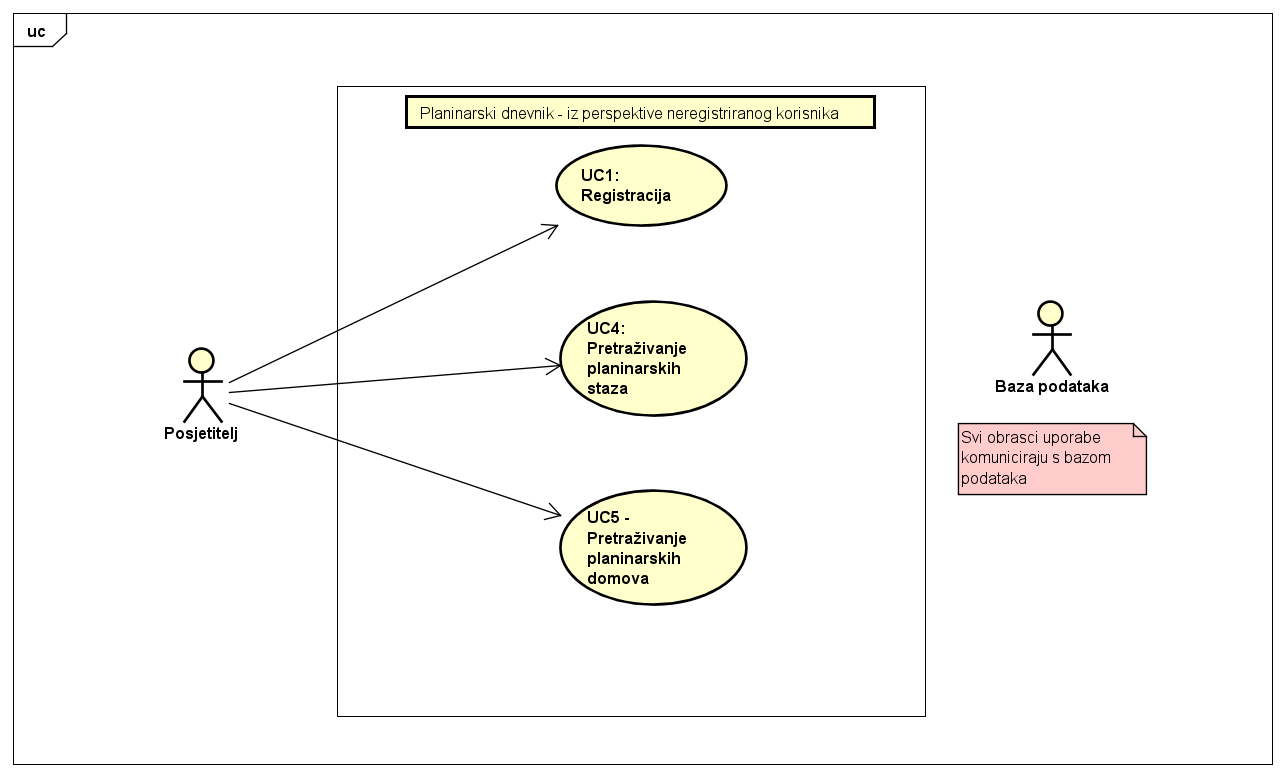
\includegraphics[scale=0.5]{dijagrami/posjetitelj-funkcionalnosti.png} %veličina slike u odnosu na originalnu datoteku i pozicija slike
					\centering
					\caption{Prikaz funkcionalnosti dostupnih neregistriranom ili neprijavljenom korisniku}
					\label{fig:UC dijagrami}
				\end{figure}
		
			\begin{figure}[H]
				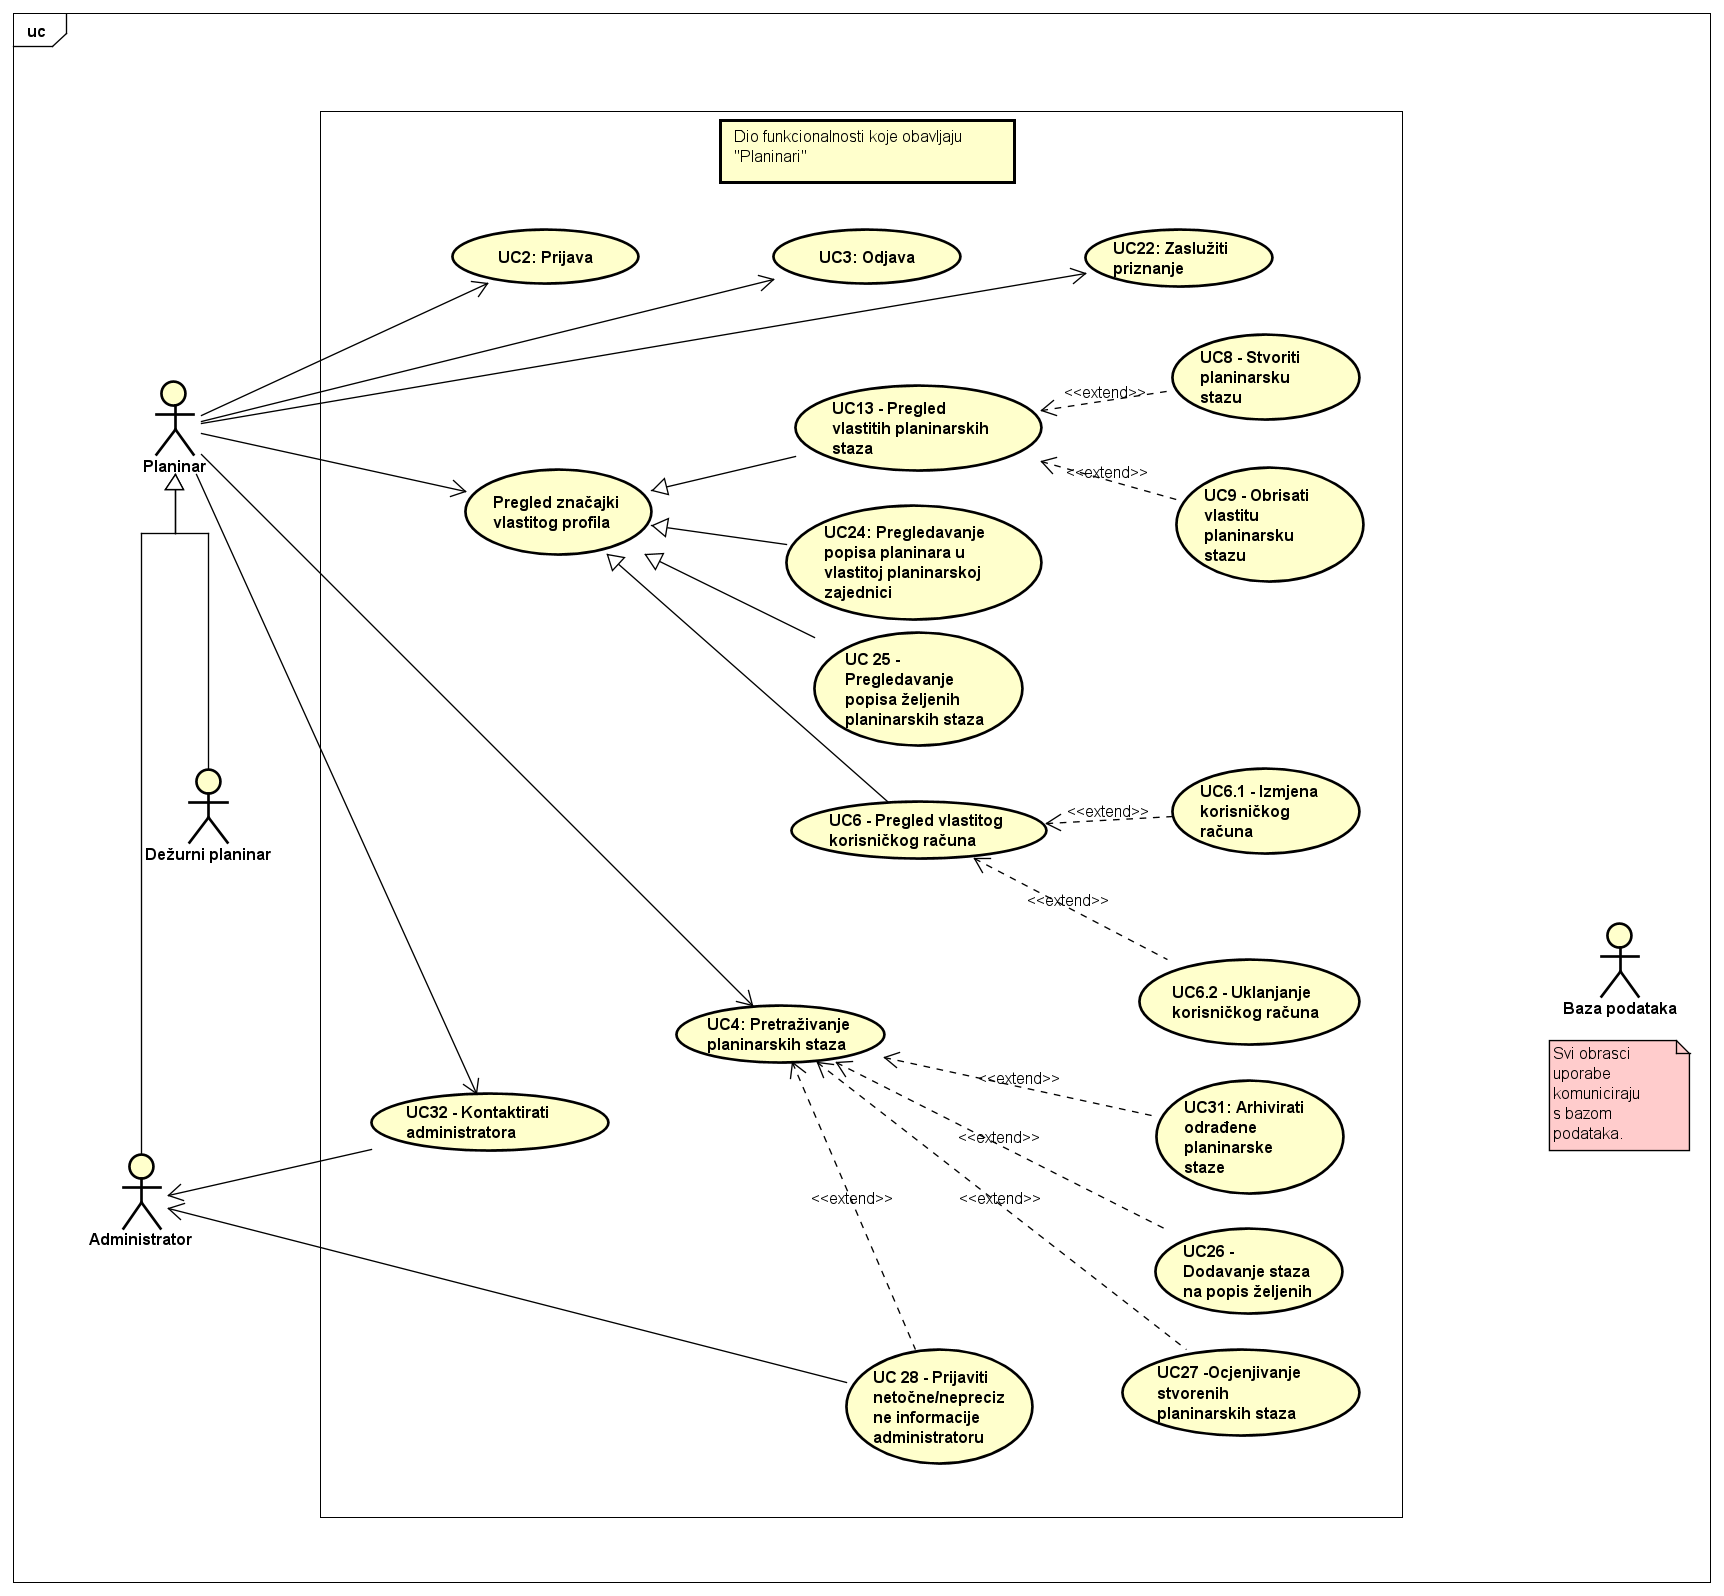
\includegraphics[scale=1, width = 165mm, height=220mm]{dijagrami/planinar1.png} %veličina slike u odnosu na originalnu datoteku i pozicija slike
				\centering
				\caption{Dio funkcionalnosti koje obavljaju planinari}
				\label{fig:UC dijagrami}
			\end{figure}
	
			\begin{figure}[H]
				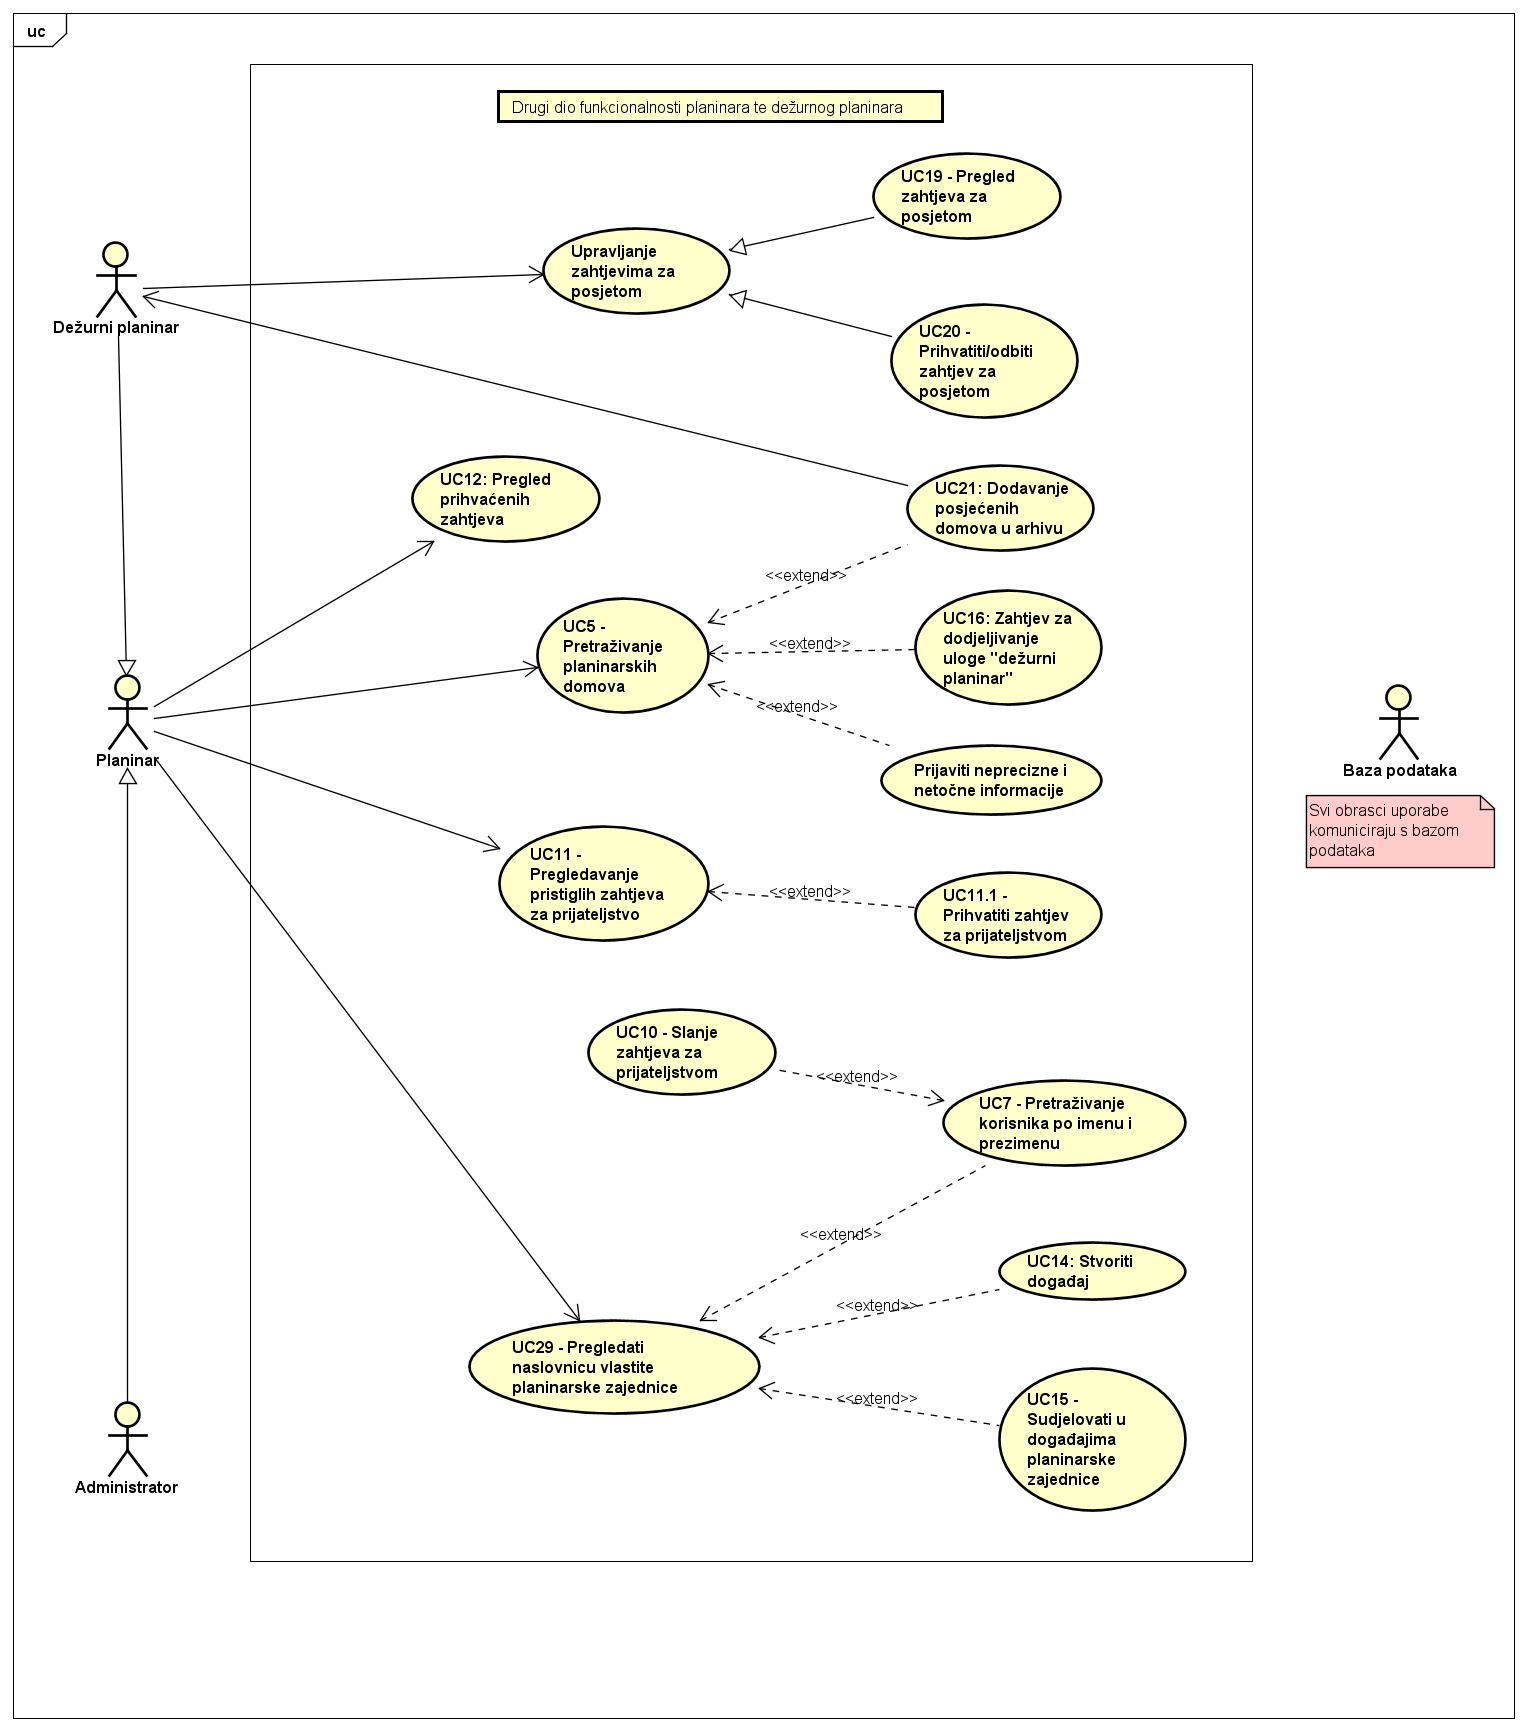
\includegraphics[scale=1, width = 165mm, height=220mm]{dijagrami/planinar2.png} %veličina slike u odnosu na originalnu datoteku i pozicija slike
				\centering
				\caption{Drugi dio funkcionalnosti planinara i zasebne aktivnosti dežurnog planinara}
				\label{fig:UC dijagrami}
			\end{figure}

		\begin{figure}[H]
			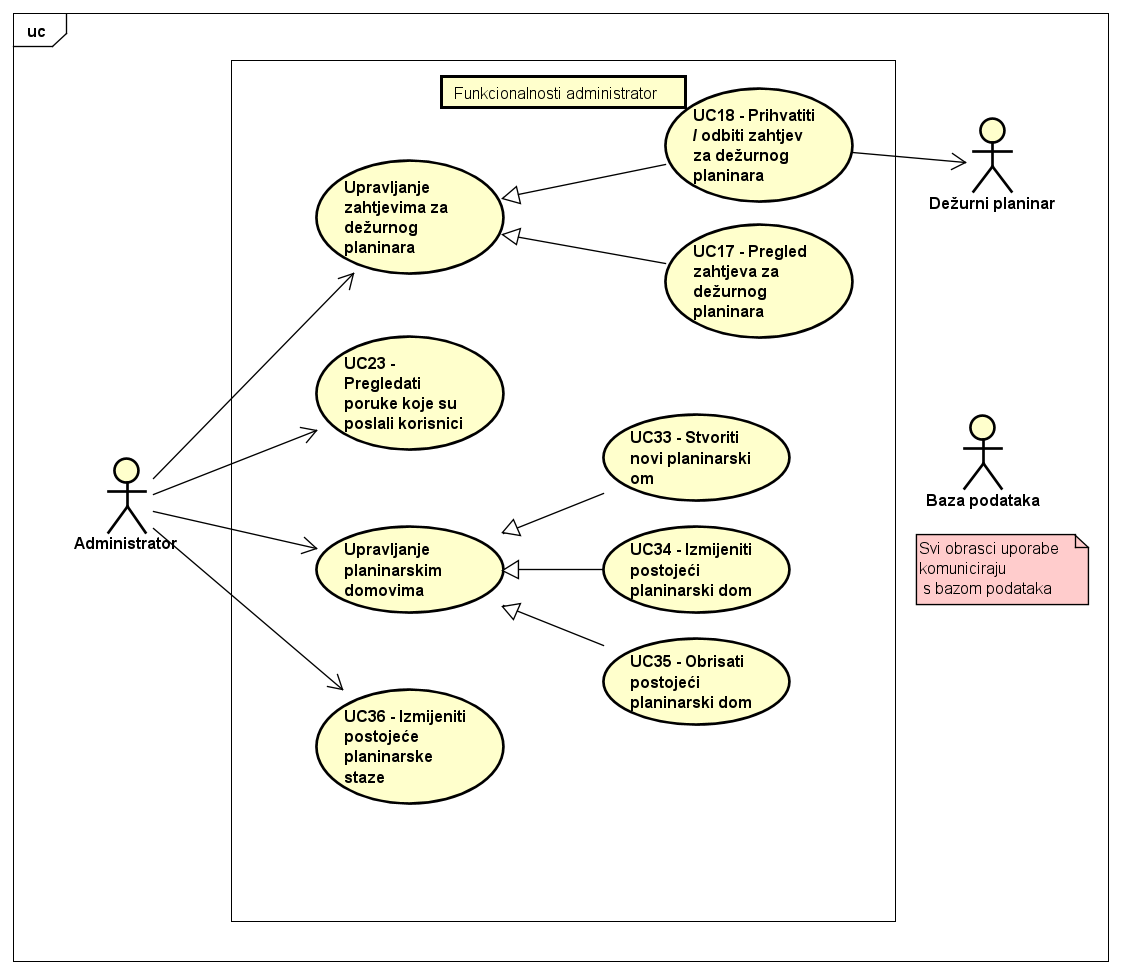
\includegraphics[scale=0.5]{dijagrami/administrator-funkcionalnosti.png} %veličina slike u odnosu na originalnu datoteku i pozicija slike
			\centering
			\caption{Prikaz funkcionalnosti koje obavlja administrator}
			\label{fig:UC dijagrami}
		\end{figure}
				
				
			\newpage	
				
			\subsection{Sekvencijski dijagrami}
			
			\subsubsection{Obrazac uporabe UC5 - Pretraživanje planinarskih domova}
			
			Korisnik odabire funkciju pregleda svih planinarskih domova. Web aplikacija, na traženi zahtjev, dohvaća planinarske domove iz baze podataka. Baza podataka zatim šalje odgovor Web aplikaciji. Odgovor baze podataka Web aplikacija prikazuje korisniku. Nadalje, ako korisnik želi užu pretragu               planinarskih domova, odabire jedan od filtera koje aplikacija nudi. Web aplikacija dohvaća iz baze podataka planinarske domove koji zadovoljavaju filtere korisnika. Baza podataka šalje listu odgovarajućih domova aplikaciji. U slučaju da je lista prazna, Web aplikacija korisniku šalje povratnu informaciju o nepostojećem domu. Ako su odgovarajući domovi pronađeni u bazi podataka Web aplikacija prikazuje listu planinarskih domova korisniku. 
				
				\begin{figure}[H]
					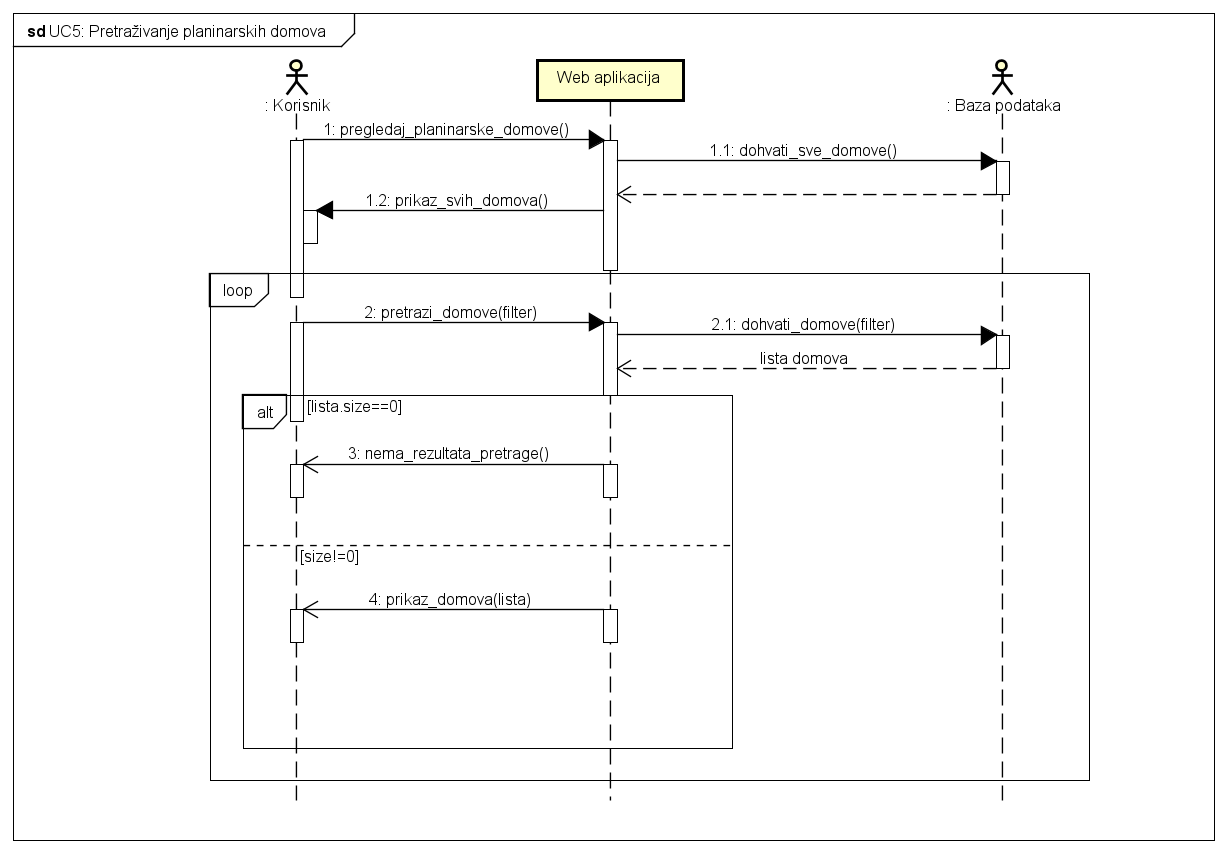
\includegraphics[scale=0.5]{dijagrami/seq-planinarski-domovi.png} %veličina slike u odnosu na originalnu datoteku i pozicija slike
					\centering
					\caption{Ponašajni prikaz pretraživanja planinarskih domova}
					\label{fig:UC dijagrami}
				\end{figure}
				
			

				\subsubsection{Obrazac uporabe UC9 - Obrisati vlastitu planinarsku stazu}

				Prijavljeni korisnik (planinar) na vlastitom profilu ima mogućnost pregleda popisa svih staza koje je stvorio. Odabirom opcije ''Moje staze'' planinar šalje zahtjev poslužitelju za prikaz tih staza. Poslužitelj dohvaća sve njegove staze iz baze podataka i prikazuje ih planinaru na njegovom profilu. Planinar zatim može odabrati stazu koju želi ukloniti tako što odabere opciju ''Ukloni stazu''. Poslužitelj u bazi podataka provjerava vidljivost odabrane staze, odnosno je li ona javna ili privatna.  Ako u bazi podataka za odabranu stazu vrijedi da je javna, onda će korisnik od poslužitelja primiti poruku da je stazu nemoguće ukloniti. Inače, ako je staza privatna, poslužitelj će korisniku postaviti pitanje: ''Jeste li sigurni da želite ukloniti stazu?'' na što planinar može odgovoriti potvrdno ili odustati od brisanja. U slučaju potvrdnog odgovora, kojeg planinar šalje poslužitelju, poslužitelj će narediti bazi podataka da ukloni odabranu stazu s popisa staza i vratit će se odgovor prema planinaru da je staza uspješno uklonjena. Ako planinar odustane od brisanja, sustav će ga vratiti na popis vlastitih staza. 

				\begin{figure}[H]
					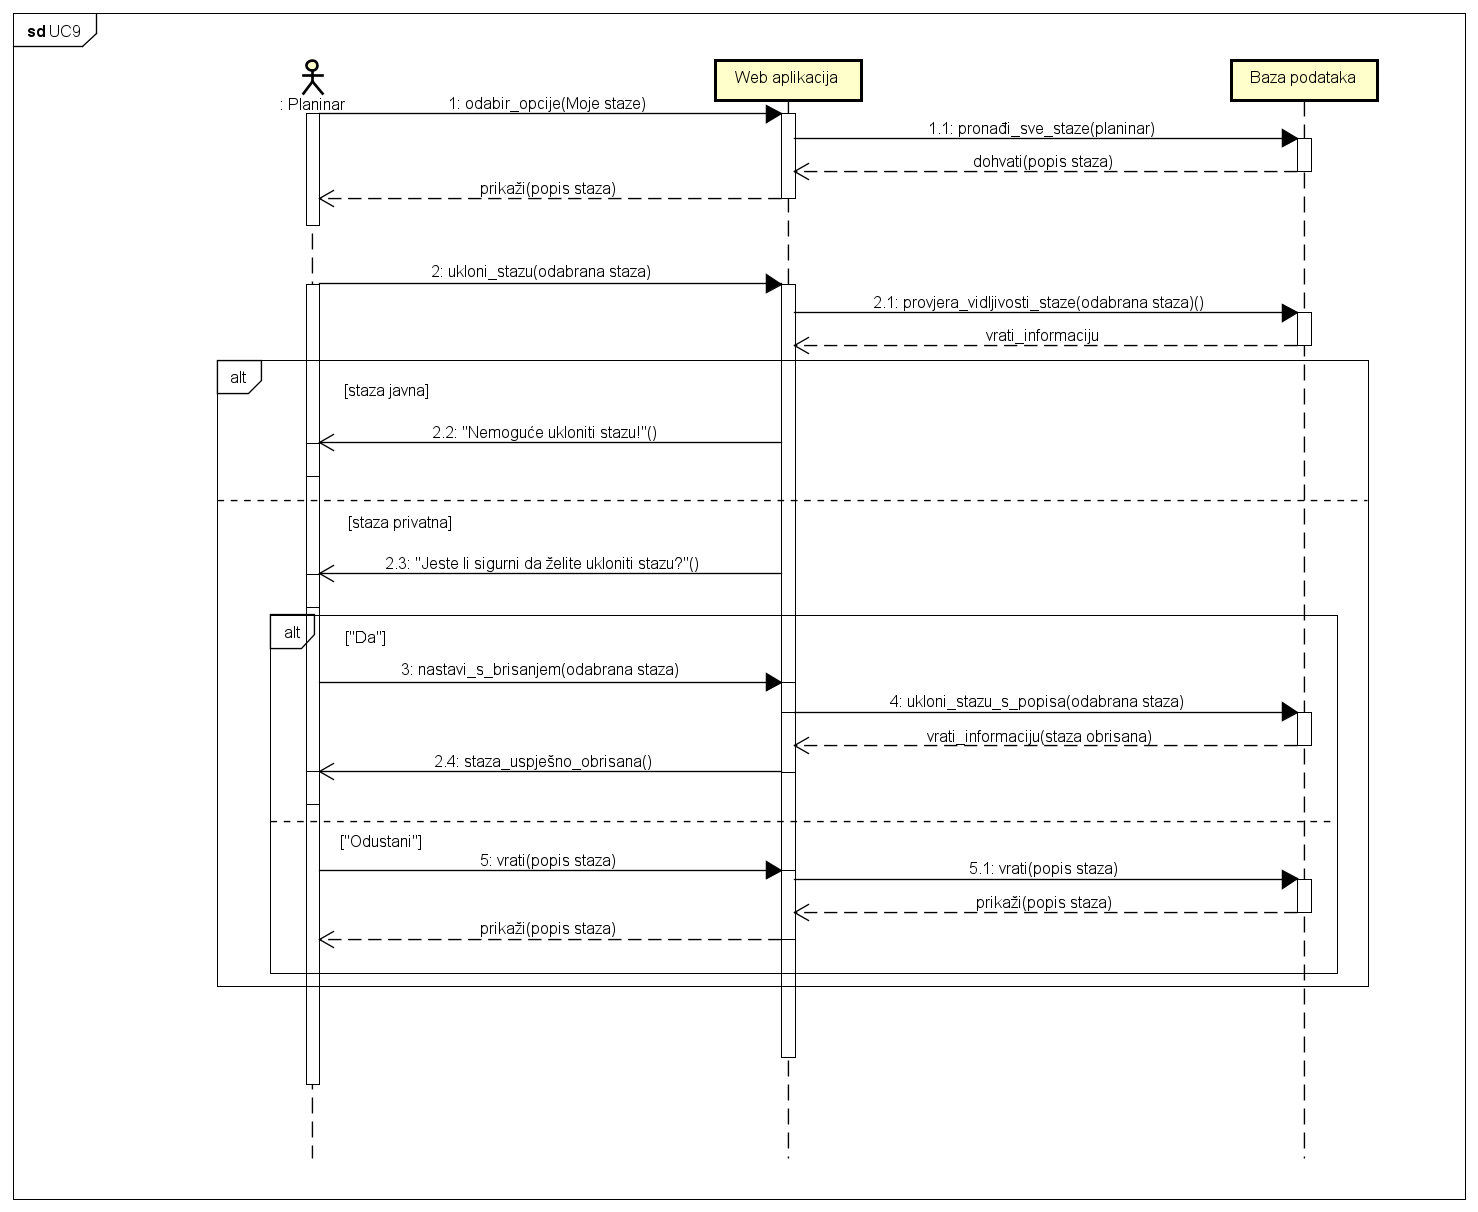
\includegraphics[scale=1.5, width=165mm, height=190mm]{dijagrami/seq-UC9.png} %veličina slike u odnosu na originalnu datoteku i pozicija slike
					\centering
					\caption{Ponašajni prikaz brisanja vlastitih planinarskih staza}
					\label{fig:sekvencijski dijagrami}
				\end{figure}
				\newpage
				\subsubsection{Obrasci uporabe UC10-UC11-UC11.1 - Zahtjevi za prijateljstvom}

				Prijavljeni korisnik (planinar) može drugom korisniku poslati zahtjev za pridruživanjem vlastitoj planinarskoj zajednici, odnosno zahtjev za prijateljstvom. Uvjet je da pošiljatelj i primatelj (planinari) imaju korisnički račun, drugim riječima da su se uspješno registrirali u aplikaciju. Planinar ima mogućnost pretraživanja drugih planinara po imenu i prezimenu. Poslužitelj će tu pretragu proslijediti bazi podataka koja će pronaći sve korisnike koji zadovoljavaju pretragu. Baza podataka vraća odgovarajuće korisnike poslužitelju koji ih onda prikazuje planinaru. Zatim planinar pošiljatelj odabire planinara iz prikazanih mu korisnika i odluči mu poslati zahtjev za prijateljstvom. Bilo koji planinar prijavljen u aplikaciju može vidjeti sve trenutno aktivne zahtjeve za prijateljstvom. U našem slučaju planinar primatelj može ili dobiti obavijest da je primio zahtjev ili može zatražiti pregled pristiglih zahtjeva. Kada planinar prima novi zahtjev poslužitelj prolongira zahtjev do planinara primatelja i vraća se povratna informacija do planinara pošiljatelja da je zahtjev uspješno poslan. Za to vrijeme u bazu podataka će se dodati taj zahtjev među aktivne zahtjeve za prijateljstvom. Ako planinar sam zatraži pregled svih zahtjeva to će napraviti tako da kontaktira poslužitelja koji će naredbu proslijediti bazi podataka. Baza podataka će tada dohvatiti aktivne zahtjeve za prijateljstvom i poslati ih poslužitelju koji će ih konačno prikazati planinaru. Planinar primatelj kod obrađivanja primljenog zahtjeva za prijateljstvo ima dvije mogućnosti: potvrditi ili odbiti zahtjev. U slučaju povrđivanja zahtjeva planinar primatelj će poslati potvrdu poslužitelju  koji će javiti planinaru primatelju da je prihvaćen njegov zahtjev za prijateljstvo. Istovremeno baza podataka će ukloniti zahtjev s popisa aktivnih zahtjeva. Ukoliko planinar primatelj odluči odbiti zahtjev, onda se taj zahtjev također uklanja s popisa aktivnih zahtjeva u bazi podataka i planinar pošiljatelj može ponovno poslati zahtjev tom istom planinaru koji ga je već odbio.
				
				\begin{figure}[H]
					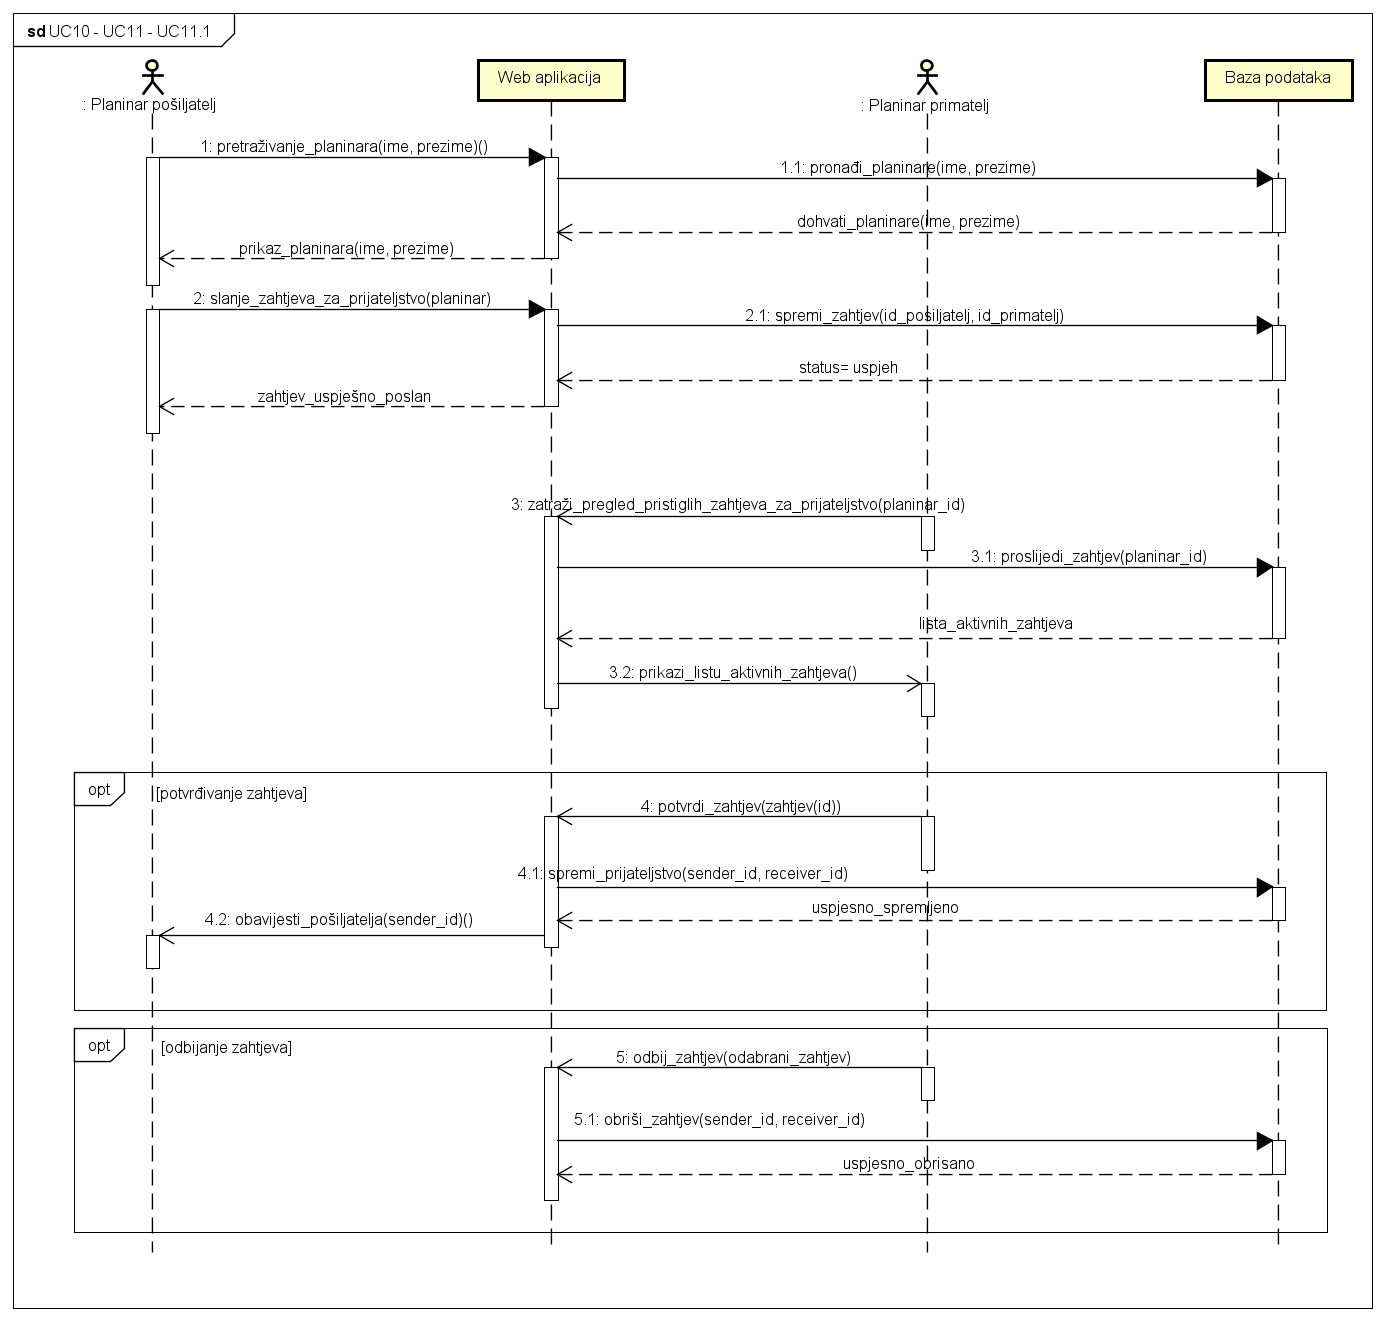
\includegraphics[scale=1.5, height=220mm, width=165mm]{dijagrami/seq-UC10 - UC11 - UC11.1.png} %veličina slike u odnosu na originalnu datoteku i pozicija slike
					\centering
					\caption{Ponašajni prikaz UC10 - UC11 - UC11.1}
					\label{fig:sekvencijski dijagrami}
				\end{figure}

				\eject
		\section{Ostali zahtjevi}
		
		 
			 	\begin{packed_item}
			 	
			 	\item  $ $Sustav treba omogućiti rad više korisnika u stvarnom vremenu $ $
			 	\item  $ $Sustav treba biti implementiran kao Web aplikacija koja će biti prilagođena i prikazu na mobilnim uređajima (aplikacija mora imati responzivan dizajn) $ $
			 	\item  $ $Korisnicima korištenje aplikacije treba biti intuitivno jasno, bez potrebe za dodatnim korisničkim uputama$ $
			 	\item  $ $Korisničko sučelje i sustav trebaju koristiti hrvatski standardni jezik (uključujući dijakritičke znakove)$ $
			 	\item  $ $Eventualne pogreške korisnika i/ili administratora ne smiju utjecati na uspješno funkcioniranje aplikacije$ $
			 	\item  $ $Baza podataka treba biti brza, učinkovita i dobro povezana sa sustavom, otporna na bilo kakve greške korisnika i administratora $ $
			 	
			 	\item  $ $Aplikacija mora biti dostupna svim zainteresiranim korisnicima, odnosno svim već aktivnim planinarima, ali i onima koji to tek namjeravaju postati$ $
			 	\item  $ $Korisnik sustavu treba moći pristupiti iz javne mreže pomoću protokola HTTPS $ $
			 	\item  $ $Nadogradnja sustava ne smije narušavati postojeće funkcionalnosti sustava$ $
			 	
			 
			 \end{packed_item}
			 
			 \eject
			 
	
	\chapter{Arhitektura i dizajn sustava}

		Arhitektura programske potpore predstavlja strukturu sustava ili više njih koje sadrži elemente, njihova obilježja i odnose među njima. Temeljni razlozi definiranja arhitekture:		

	\begin{itemize}
		\item 	{poboljšava razumljivost i komunikaciju sudionika}
		\item 	{pomaže u donošenju temeljnih odluka pri izradi projekta}
		\item 	{omogućava rano uočavanje pogrešaka u oblikovanju}		
		\item         {moguće ponovno korištenje rješenja (engl. reuse)}
	\end{itemize}

	U konačnici, efikasno strukturiranje arhitekture programske potpore dovest će do poboljšanja kvalitete finalnog produkta projekta.

	\vspace{10mm} %10mm vertical space

	Koristimo objektno usmjerenu arhitekturu koja najbolje odgovara razvoju složene Web aplikacije namijenjene za što više korisnika u stvarnom vremenu. Možemo ju klasificirati na četiri ključna dijela koji osiguravaju izvršavanje naredbi korisnika: 
		
	\begin{packed_enum}
		\item 	{Web preglednik}
		\item 	{Web poslužitelj}
		\item 	{Web aplikacija}
		\item 	{Baza podataka}
	\end{packed_enum}			

		\begin{figure}[H]
					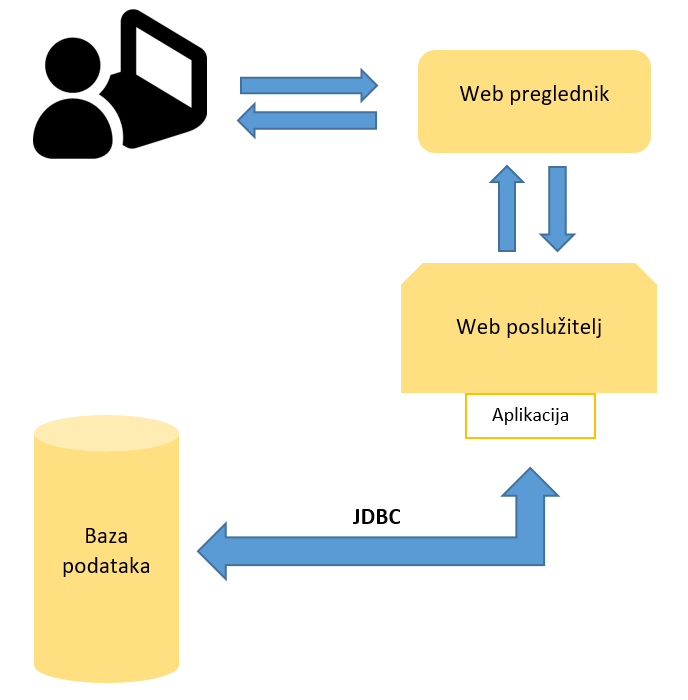
\includegraphics[scale=0.8]{arhitektura/arhitektura_sustava.png} %veličina slike u odnosu na originalnu datoteku i pozicija slike
					\centering
					\caption{Arhitektura sustava}
					\label{fig:arhitektura}
		\end{figure}

	\vspace{5mm} %5mm vertical space

		Web aplikacija će se temeljiti na modelu klijent-poslužitelj, što je danas i najčešće korišteni model. Korisnik šalje zahtjeve na koje odgovara poslužitelj, dok i jedna i druga strana mogu imati korisničku i poslužiteljsku aplikaciju.

	\vspace{10mm} %10mm vertical space

		\textbf{\underline{Web preglednik:} }\\

			Klijentski program, zvan preglednik, služi kao korisničko sučelje za pregledavanje sadržaja na Webu. On je taj koji šalje zahtjev Web poslužitelju i prikazuje primljene podatke u obliku Web stranica korisniku. Dakle, preglednik će primljene podatke u obliku koda interpretirati u nešto korisniku razumljivo, odnosno prikazat će korisničko sučelje naše aplikacije. Konačan prikaz aplikacije može uključivati više dohvata resursa i često može sadržavati dodatke te pomoćne aplikacije za prikaz formata koje izvorno ne podržava.

		\vspace{5mm} %5mm vertical space
		\textbf{\underline{Web poslužitelj:} }\\

		Poslužiteljski program poslužuje resurse smještene na poslužiteljskom računalu ili na drugim izvorima i odgovara na zahtjeve korisnika. Komunikacija se odvija preko HTTP/HTTPS (\textit{HyperText Transfer Protocol/Secure}) standardnog internetskog aplikacijskog protokola koji ima mogućnost prijenosa raznih vrsta podataka i proširiv je prema novim formatima podataka. Poslužitelj je zaslužan za pokretanje Web aplikacije.

		\vspace{5mm} %5mm vertical space
		
		\textbf{\underline{Web aplikacija:} }\\

		Za realizaciju frontend-a, odnosno korisničkog sučelja upotrijebit ćemo React kao bazu unutar kojega ćemo koristiti jezike HTML, TypeScript i CSS. TypeScript nam omogućava izradu dinamičkih web stranica u kombinaciji s HTML-om i CSS-om i njime možemo mijenjati sadržaj na stranici ovisno o načinu interakcije korisnika sa stranicom. Uz ove navedene tehnologije moguće je napraviti moderno korisničko sučelje jedne Web i mobilne aplikacije. Nakon što Web preglednik korisniku prikaže aplikaciju ''Planinarski dnevnik'', korisnik može izvršiti određenu naredbu odabirom neke od funkcionalnosti aplikacije. Hoće li pristupiti bazi podataka ovisi o samoj akciji. Za komunikaciju s bazom podataka koristi se JDBC koji predstavlja sučelje aplikacijskog programiranja za jezik Java i definira kako klijent može pristupiti bazi podataka. Pruža metode za upit i ažuriranje u bazi podataka te je orijentiran prema relacijskim bazama podataka. Što se tiče backend-a koristimo Spring Boot i MVC arhitekturu. 


		\vspace{5mm} %5mm vertical space

		\textbf{Spring Boot} pruža fleksibilan način konfiguriranja Java Beans, XML konfiguracija i transakcija baze podataka te bitno olakšava upravljanje ovisnostima. Svaka pokrenuta usluga ima svoj postupak, a time se postiže jednostavan model za podršku aplikacijama.  


		\vspace{5mm} %5mm vertical space

		\textbf{Model – View – Controller} je obrazac koji razdvaja aplikaciju u tri glavne logičke komponente: Model, View i Controller. Svaka od nabrojenih komponenti ima zadatak rukovati s određenim razvojnim aspektima aplikacije. Također, one su nezavisne jedna od druge i kao rezultat toga je jednostavno dodavanje i preoblikovanje svojstava.


		\vspace{5mm} %5mm vertical space

		\begin{itemize}
		\item \textbf{Model}	
		
		Poznat je kao najniža razina što znači da je odgovoran za održavanje podataka s kojima korisnik radi. Glavni zadatak je dohvat, manipulacija podatcima i uglavnom on surađuje s bazom podataka. Reagira na zahtjeve Controller-a jer on nikada sam ne razgovara s bazom podataka i nakon komunikacije prosljeđuje potrebne podatke Controllor-u. Jedna od bitnijih stvari za napomenuti je da Model nikada izravno ne komunicira s View.

		\item \textbf{View}
		
		Služi za prikazivanje podataka na način da zapravo generira korisničko sučelje za korisnika. Ti podaci su rezultat rada Model-a, ali se oni ne preuzimaju izravno već putem Controller-a tako da View surađuje samo s Controller-om. 

		\item \textbf{Controller}

		Djeluje u službi posrednika između komponenti Model i View. Ne mora brinuti o rukovanju logikom podataka, već samo govori Model-u što treba učiniti. Nakon primanja podataka od Model-a, on ih obrađuje i konačno rezultat prosljeđuje do View-a gdje objašnjava kako ih prikazati korisniku. Ako je došlo do promjena, Controller je zadužen za ažuriranje View-a.


		\end{itemize}


		\begin{figure}[H]
					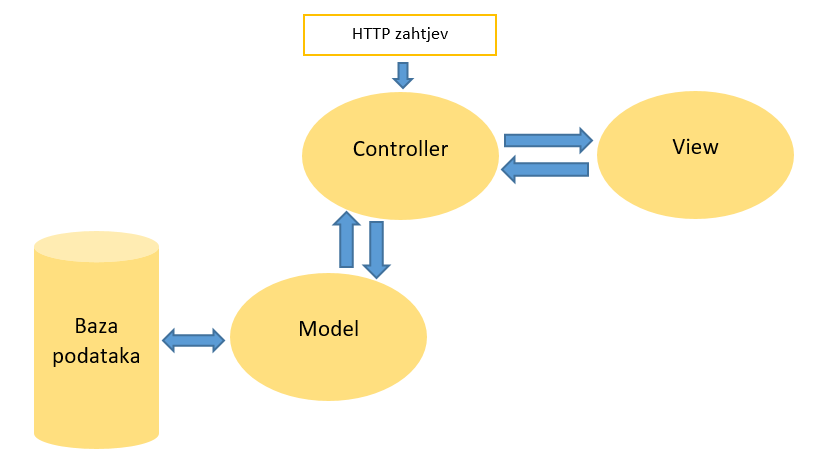
\includegraphics[scale=0.8]{arhitektura/mvc.png} %veličina slike u odnosu na originalnu datoteku i pozicija slike
					\centering
					\caption{Model - View - Controller}
					\label{fig:arhitektura}
		\end{figure}

		\section{Baza podataka}
			
		Za naš projekt odabrali smo \textbf{relacijsku bazu podataka} zbog njezine pogodnosti da prikaže mali dio stvarnog svijeta bez redundancije unutar same baze. Dohvaćanje podataka je relativno brzo i lagano se može paralelizirati. Specifičnu implementaciju relacijske baze podataka koju smo odabrali je \textbf{PostgreSQL}. To je baza podataka otvorenog koda s preko 30 godina aktivnog razvoja zbog kojeg je zaslužila svoju čvrstu reputaciju za pouzdanost, bogatstvo opcijama i visokim performansama. Zbog načina na koji je SQL standard napisan, vrlo je slična ostalim SQL bazama podataka.\\ 
		
		Tijekom razvoja koristimo \textbf{H2 bazu}. To je privremena baza podataka koja služi za testiranje koda. Svi zapisi u njoj se nalaze u privremenoj memoriji i nisu perzistentni. Zbog toga je odlična za testiranje. Ona je otvorenog koda, napisana u Javi i ima čvrste sigurnosne postavke. Na nju se možemo povezati s više konekcija i baza podataka je enkriptirana SHA-256 enkripcijom. Ima vrlo malu potrošnju memorije i zauzima relativno malo prostora na disku (oko 2MB). \\ 
		
		Također koristimo \textbf{JPA (Java Persistence API)} koje samo sadrži sučelja za stvaranje Persistence layouta. Dopušta nam da mapiramo entitete tablica i veze između tablica na objekte u Javi. Ovo sučelje definira svoj vlastiti jezik za upite (JPQA). JPQA prevoditelj interpretira kod i piše SQL upite. JPA ne možemo samostalno koristiti, već nam treba konkretna implementacija toga sučelja. Implementacija koju ćemo mi koristiti se zove Hibernate. \\ 
		
		Na bazu podataka se iz Jave spajamo preko \textbf{JdbcTemplatea}. To je snažni mehanizam za spajanje i izvođenje SQL upita. On nam smanjuje količinu koda koju moramo napisati kako bismo izvršavali upite, kao što je spajanje na bazu, kreiranje izraza i zatvaranje konekcija. \\
		\newpage
	Naš model baze podataka sastoji se od sljedećih \textbf{glavnih} i \underline{veznih} tablica:
		\begin{itemize}[noitemsep]
		\item \textbf{user}
		\item \textbf{residence$\_$place}
		\item \textbf{role}
		\item \textbf{mountain$\_$lodge}
		\item \textbf{mountain$\_$path}
		\item \textbf{event}
		\item \textbf{hill}
		\item \textbf{utility}
		\item \textbf{badge}
		\item \textbf{contact$\_$message}
		\item \underline{visit$\_$confirmation}
		\item \underline{friendships}
		\item \underline{frienship$\_$req}
		\item \underline{user$\_$role}
		\item \underline{user$\_$place}
		\item \underline{user$\_$badge}
		\item \underline{mountain$\_$lodge$\_$utility}
		\item \underline{mountain$\_$lodge$\_$report}
		\item \underline{duty$\_$mountaneer}
		\item \underline{event$\_$path}
		\item \underline{event$\_$attendance}
		\item \underline{mountain$\_$path$\_$report}
		\item \underline{mountain$\_$path$\_$grade}
		\item \underline{path$\_$user$\_$wishlist}
		\item \underline{mountain$\_$path$\_$completed}
		\item \underline{badge\_notification}

\end{itemize}
		 \newpage
			\subsection{Opis tablica}
			Primarni ključevi su označeni \textbf{podebljano}, dok su strani ključevi \underline{podvučeni}. \\
			Prikazane su i sve vezne tablice, tako da se nad glavnim tablicama Many-To-Many veze neće navoditi.
			
%Tablice
			\textbf{user} -  ovaj entitet sadrži sve važne informacije o korisniku aplikacije.
			Sadrži atribute: "id", "full$\_$name", "email", "password", "image", "id$\_$place", "date$\_$of$\_$birth" i "description" koji redom predstavljaju jedinstveni identifikacijski broj korisnika, ime i prezime, e-mail korisnika, lozinku korisnika, sliku vidljivu na profilu korisnika, identifikacijski broj mjesta stanovanja korisnika te datum rođenja korisnika.
			Neki podaci o korisniku, kao što su mjesto stanovanja i datum rođenja su opcionalni, i ako ih korisnik ne ispuni njihova vrijednost je \textit{NULL}. Atribut "place\_id" je strani ključ koji referencira entitet \textbf{residence\_place} te se radi o Many-To-One vezi. 
			
			\begin{longtabu} to \textwidth {|X[6, l]|X[6, l]|X[20, l]|}
				\hline \multicolumn{3}{|c|}{\textbf{user - (Korisnik)}}	 \\[3pt] \hline
				\endfirsthead
				
				\hline \multicolumn{3}{|c|}{\textbf{user - (Korisnik)}}	 \\[3pt] \hline
				\endhead
				
				\hline 
				\endlastfoot
				
				\textbf{id} & BIGINT	&  	jedinstveni identifikacijski broj korisnika	\\ \hline
				full$\_$name	& VARCHAR &  ime i prezime korisnika 	\\ \hline 
				email & VARCHAR &  e-mail pomoću kojeg se korisnik prijavljuje u sustav \\ \hline 
				password & VARCHAR	&  	lozinka pomoću koje se korisnik prijavljuje u sustav	\\ \hline 
				image & BYTEA	&  	slika vidljiva na profilu korisnika	\\ \hline 
				\underline{place\_id} & BIGINT & strani ključ mjesta stanovanja korisnika iz tablice \textbf{residence\_place}, unos je opcionalan\\ \hline
				date\_of\_birth & DATE & datum rođenja korisnika, unos je opcionalan \\ \hline
				
				
			\end{longtabu}
			\vspace{10mm}
			
			\textbf{residence\_place}  Ovo je entitet koji modelira mjesto stanovanja korisnika. Sadrži atribute: "id" i "name" koji predstavljaju jedinstveni identifikator mjesta te naziv mjesta.
			
			
			\begin{longtabu} to \textwidth {|X[6, l]|X[6, l]|X[20, l]|}
				
				\hline \multicolumn{3}{|c|}{\textbf{residence\_place - (Mjesto stanovanja)}}	 \\[3pt] \hline
				\endfirsthead
				
				\hline \multicolumn{3}{|c|}{\textbf{residence\_place - (Mjesto stanovanja)}}	 \\[3pt] \hline
				\endhead
				
				\hline 
				\endlastfoot
				
				\textbf{id} & BIGINT	&  	jedinstveni indetifikacijski broj mjesta stanovanja	\\ \hline
				name	& VARCHAR &  naziv mjesta 	\\ \hline 
				%\cellcolor{LightBlue} primjer	& VARCHAR &   	\\ \hline 
				
				
			\end{longtabu}
				
				\vspace{10mm}
			\newpage
			\textbf{role} Ovaj entitet modelira ulogu korisnika unutar aplikacije, tzv. "aplikativne role". Određuje razinu ovlasti koje korisnik ima. Sadrži atribute: "id" i "name" koji predstavljaju jedinstveni identifikator uloge te naziv uloge. Dopuštene uloge u našoj aplikaciji su: Planinar, Dežurni planinar i Administrator.
			
			\begin{longtabu} to \textwidth {|X[6, l]|X[6, l]|X[20, l]|}
				
				\hline \multicolumn{3}{|c|}{\textbf{role - (Uloga)}}	 \\[3pt] \hline
				\endfirsthead
				
				\hline \multicolumn{3}{|c|}{\textbf{role - ime tablice}}	 \\[3pt] \hline
				\endhead
				
				\hline 
				\endlastfoot
				
				\textbf{id} & BIGINT	&  jedinstveni ID uloge	\\ \hline
				name	& VARCHAR &  ime uloge 	\\ \hline 
				
			\end{longtabu}
		
		\vspace{10mm}		
		
		\textbf{mountain\_lodge} Ovaj entitet modelira jedan planinarski dom. Sadrži atribute: "id", "name", "image", "elevation" i "hill\_id" koji predstavljaju jedinstveni identifikator planinarskog doma, naziv planinarskog doma, sliku planinarskog doma, nadmorsku visinu te jedinstveni identifikator zemljopisnog područja (visočja) na kojemu se planinarski dom nalazi. Unos slike za neki planinarski dom je opcionalan, a ako se atribut ne popuni njegova vrijednost je \textit{NULL}. Atribut "hill\_id" predstavlja strani ključ koji referencira entitet \textbf{hill} te se radi o Many-To-One vezi. 
		
		\begin{longtabu} to \textwidth {|X[6, l]|X[6, l]|X[20, l]|}
			
			\hline \multicolumn{3}{|c|}{\textbf{mountain\_lodge - (Planinarski dom)}}	 \\[3pt] \hline
			\endfirsthead
			
			\hline \multicolumn{3}{|c|}{\textbf{mountain\_lodge - ime tablice}}	 \\[3pt] \hline
			\endhead
			
			\hline 
			\endlastfoot
			
			\textbf{id} & BIGINT	&  	jedinstveni identifikacijski broj planinarskog doma 	\\ \hline
			name	& VARCHAR &   naziv planinarskog doma	\\ \hline 
			image & BYTEA &  slika planinarskog doma koja se prikazuje unutar aplikacije, unos je opcionalan \\ \hline 
			elevation & INTEGER & nadmorska visina na kojoj se planinarski dom nalazi izražena u kilometrima \\ \hline 
			\underline{hill\_id} & BIGINT	&  strani ključ na tablicu \textbf{hill}, a predstavlja identifikator visočja na kojemu se nalazi planinarski dom	\\ \hline 
			
			
		\end{longtabu}
	\vspace{10mm}		
	
	
	\textbf{utility} Ovaj entitet modelira značajke infrastrukture pojedinog doma. Sadrži atribute "id" i "name" koji predstavljaju jedinstveni identifikacijski broj značajke te naziv značajke. Primjeri takvih značajki su pitka voda, hrana, smještaj, internet.
	
	\newpage
	\begin{longtabu} to \textwidth {|X[6, l]|X[6, l]|X[20, l]|}
		
		\hline \multicolumn{3}{|c|}{\textbf{utility - (Pogodnost, značajka)}}	 \\[3pt] \hline
		\endfirsthead
		
		\hline \multicolumn{3}{|c|}{\textbf{utility - ime tablice}}	 \\[3pt] \hline
		\endhead
		
		\hline 
		\endlastfoot
		
		\textbf{id} & BIGINT	&  jedinstveni identifikator značajke\\ \hline
		name	& VARCHAR &  naziv značajke/pogodnosti \\ \hline 
		
	\end{longtabu}
				\vspace{10mm}		
				
				\textbf{hill} Ovaj entitet modelira pojedino zemljopisno područje, odnosno visočje na kojemu se nalazi pojedini planinarski dom ili planinarska staza. Sadrži atribute: "id" i "name" koji predstavljaju jedinstveni identifikacijski broj visočja te naziv visočja.
				
				\begin{longtabu} to \textwidth {|X[6, l]|X[6, l]|X[20, l]|}
					
					\hline \multicolumn{3}{|c|}{\textbf{hill - (Visočje)}}	 \\[3pt] \hline
					\endfirsthead
					
					\hline \multicolumn{3}{|c|}{\textbf{hill - ime tablice}}	 \\[3pt] \hline
					\endhead
					
					\hline 
					\endlastfoot
					
					\textbf{id} & BIGINT	&  jedinstveni ID visočja 	\\ \hline
					name & VARCHAR	&  ime visočja 	\\ \hline
					
					
				\end{longtabu}
				\vspace{10mm}
			
			\textbf{mountain\_path} Ovaj entitet sadrži informacije o pojedinoj planinarskoj stazi. Sadrži atribute: "id", "name", "start\_point", "end\_point", "avg\_walk\_time", "length", "sea\_level\_diff", "date\_created", "is\_private", "author\_id" i "hill\_id" koji redom predstavljaju jedinstveni identifikacijski broj planinarske staze, naziv staze, polazišnu točku, završnu toku, prosječno vrijeme potrebno da se prepješači staza, duljinu staze, razliku u nadmorskoj visini između početne i završne točke, datum kreiranja pojedine staze od strane korisnika unutar naše aplikacije, vrijednost koja govori je li staza privatna ili javna, korisnika koji je stvorio stazu te identifikator visočja na kojemu se staza nalazi. Atribut "author\_id" te atribut "hill\_id" su strani ključevi obzirom na tablicu \textbf{user} odnosno \textbf{hill} te se radi o Many-To-One vezama.
			
			\begin{longtabu} to \textwidth {|X[6, l]|X[6, l]|X[20, l]|}
				
				\hline \multicolumn{3}{|c|}{\textbf{mountain\_path - (Planinarska staza)}}	 \\[3pt] \hline
				\endfirsthead
				
				\hline \multicolumn{3}{|c|}{\textbf{mountain\_path - (Planinarska staza)}}	 \\[3pt] \hline
				\endhead
				
				\hline 
				\endlastfoot
				
				\textbf{id} & BIGINT	& jedinstveni identifikacijski broj planinarske staze	\\ \hline
				name	& VARCHAR &  naziv staze	\\ \hline 
				start\_point & VARCHAR & naziv početne točke staze  \\ \hline 
				end\_point & VARCHAR &  naziv završne točke staze \\ \hline 
				avg\_walk\_time & TIME &  prosječno vrijeme potrebno za prepješačiti stazu\\ \hline 
				length & INTEGER & duljina staze u metrima\\ \hline 
				sea\_level\_diff & INTEGER & razlika u nadmorskoj visini između početne i završne točke staze\\ \hline 
				date\_created & DATE &  datum stvaranja staze unutar aplikacije\\ \hline 
				is\_private & BOOLEAN	&  atribut koji govori je li korisnik stazu stvara privatno ili javno  \\ \hline 
				\underline{author\_id} & BIGINT	&  	identifikacijski broj korisnika koji je stvorio stazu unutar aplikacije\\ \hline 
				\underline{hill\_id} & BIGINT	&  identifikacijski broj visočja na kojemu se staza nalazi\\ \hline 
				
				
			\end{longtabu}
			\vspace{10mm}
			
			\textbf{event} Ovaj entitet modelira jedan događaj koji stvara korisnik unutar naše aplikacije. Jedan događaj počinje u određeno vrijeme "start\_date", te završava u određeno vrijeme: "end\_date". Svaki događaj, odnosno planinarski izlet sastoji se od jedne ili više planinarskih staza koje se obilaze tijekom tog planinarskog izleta. Osim toga, planinarski izlet ima svoj opis: "description", gdje korisnik može reći više pojedinosti o samom planinarskom izletu. Osim toga, ovaj entitet sadrži atribute: "id", "name", "date\_created" i "author\_id" koji predstavljaju jedinstveni identifikacijski broj događaja, naziv događaja, vrijeme kada je korisnik stvorio događaj unutar aplikacije te jedinstveni identifikacijski broj korisnika koji je stvorio događaj. Atribut "author\_id" je strani ključ koji se odnosi na tablicu \textbf{user} te se radi o Many-To-One vezi.
			
			\begin{longtabu} to \textwidth {|X[6, l]|X[6, l]|X[20, l]|}
				
				\hline \multicolumn{3}{|c|}{\textbf{event - (Planinarski događaj)}}	 \\[3pt] \hline
				\endfirsthead
				
				\hline \multicolumn{3}{|c|}{\textbf{event - (Planinarski događaj)}}	 \\[3pt] \hline
				\endhead
				
				\hline 
				\endlastfoot
				
				\textbf{id} & BIGINT	&  	jedinstveni identifikacijski broj planinarskog izleta 	\\ \hline
				name	& VARCHAR & naziv događaja 	\\ \hline 
				description & VARCHAR &  pojedinosti vezane uz događaj \\ \hline 
				start\_date & TIMESTAMP	&  vrijeme i datum početka planinarskog izleta	\\ \hline 
				end\_date & TIMESTAMP	&  	vrijeme i datum završetka planinarskog izleta	\\ \hline 
				date\_created & TIMESTAMP	&  vrijeme i datum stvaranja izleta unutar aplikacije\\ \hline 
				\underline{author\_id} & BIGINT	& jedinstveni identifikacijski broj korisnika koji je stvorio događaj unutar aplikacije		\\ \hline 
				
				
			\end{longtabu}
			\vspace{10mm}
			
			\textbf{badge} Ovaj entitet modelira jedan bedž, odnosno priznanje koje korisnik može zaslužiti kao planinar. Korisnik priznanja zaslužuje za svoju aktivnost koja se gleda na osnovu arhive planinarskih domova i staza, te se uzimaju u obzir značajke kao što su: broj posjećenih planinarskih domova, broj odrađenih planinarskih staza i sl. Entitet sadrži atribute "id" i "name" koji predstavljaju jedinstveni identifikacijski broj priznanja te naziv priznanja.
			
			\begin{longtabu} to \textwidth {|X[6, l]|X[6, l]|X[20, l]|}
				
				\hline \multicolumn{3}{|c|}{\textbf{badge - (Priznanje)}}	 \\[3pt] \hline
				\endfirsthead
				
				\hline \multicolumn{3}{|c|}{\textbf{badge - (Priznanje)}}	 \\[3pt] \hline
				\endhead
				
				\hline 
				\endlastfoot
				
				\textbf{id}	& BIGINT &   jedinstveni identifikacijski broj priznanja	\\ \hline 
				name & VARCHAR &  naziv priznanja \\ \hline 
				
				
			\end{longtabu}
		
				\vspace{10mm}
				
				\textbf{contact\_message} Ovaj entitet modelira poruke koje korisnik može slati administratoru u slučaju npr. otvaranja novog planinarskog doma. Sadrži atribute: "id", "description", "date\_send" koji redom predstavljaju jedinstveni identifikacijski broj poruke, opis odnosno sadržaj poruke te datum i vrijeme slanja poruke.
				
				\begin{longtabu} to \textwidth {|X[6, l]|X[6, l]|X[20, l]|}
					
					\hline \multicolumn{3}{|c|}{\textbf{contact\_message - (Poruke administratoru)}}	 \\[3pt] \hline
					\endfirsthead
					
					\hline \multicolumn{3}{|c|}{\textbf{badge - (Priznanje)}}	 \\[3pt] \hline
					\endhead
					
					\hline 
					\endlastfoot
					
					\textbf{id}	& BIGINT &   jedinstveni identifikacijski broj poruke	\\ \hline 
					description & VARCHAR &  sadržaj poruke \\ \hline 
					created\_on & DATE &  datum i vrijeme slanja poruke \\ \hline 
					\underline{user\_id} & BIGINT	& jedinstveni identifikacijski broj korisnika koji je stvorio poruku unutar aplikacije		\\ \hline 
					
				\end{longtabu}
				\vspace{10mm}
				
				
				
				\textbf{visit\_confirmation} Ovo je vezna tablica koja nam modelira zahtjeve koje korisnik šalje dežurnim planinarima kada je posjetio određeni dom. Tablica predstavlja Many-To-Many vezu između entiteta \textbf{user} i entiteta \textbf{mountain\_lodge}. Osim stranih ključeva "user\_id" i "lodge\_id" sadrži i atribute "time\_requested" i "status" koji redom predstavljaju vrijeme slanja zahtjeva te status obrade zahtjeva za posjetom, koji može biti: ACCEPTED (Prihvaćen), REJECTED (Odbijen) ili PENDING (Aktivan).
				
				\begin{longtabu} to \textwidth {|X[6, l]|X[6, l]|X[20, l]|}
					
					\hline \multicolumn{3}{|c|}{\textbf{visit\_confirmation - (Zahtjev za potvrdom posjeta)}}	 \\[3pt] \hline
					\endfirsthead
				
					\hline 
					\endlastfoot
					
					\underline{user\_id} & BIGINT	&  strani ključ korisnika koji traži potvrdu posjeta iz tablice \textbf{user}\\ \hline
					\underline{lodge\_id}	& BIGINT & strani ključ planinarskog doma kojeg posjećuje iz tablice \textbf{mountain\_lodge} 	\\ \hline 
					time\_requested & TIMESTAMP &  datum i vrijeme slanja zahtjeva za posjetom \\ \hline 
					status & VARCHAR	&  status zahtjeva	\\ \hline  
		
		\end{longtabu}
		\vspace{10mm}
	
			\textbf{friendships} Ovo je vezna tablica koja sadrži Many-To-Many vezu između dva korisnika, a služi nam za modeliranje prijateljstava, odnosno pripadanja istoj planinarskoj zajednici. Sadrži atribute "user\_id1" i "user\_id2" koji predstavljaju strane ključeve na tablicu \textbf{user} i govore nam tko su korisnici koji pripadaju istoj zajednici, te atribut "friendship\_created" koji nam govori o datumu i vremenu stvaranja prijateljstva.
			
			\begin{longtabu} to \textwidth {|X[6, l]|X[6, l]|X[20, l]|}
				
				\hline \multicolumn{3}{|c|}{\textbf{friendships - (Prijatelji)}}	 \\[3pt] \hline
				\endfirsthead
				
				\hline \multicolumn{3}{|c|}{\textbf{friendships - (Prijatelji)}}	 \\[3pt] \hline
				\endhead
				
				\hline 
				\endlastfoot
				
				\underline{user\_id1} & BIGINT	&  strani ključ koji se odnosi na jednog korisnika člana veze "prijatelji"	\\ \hline
				\underline{user\_id2}	& BIGINT &   strani ključ koji se odnosi na drugog korisnika člana veze "prijatelji"\\ \hline 
				friendship$\_$ \text{created}	& TIMESTAMP &   vrijeme i datum kada su dva određena korisnika postala prijatelji	\\ \hline 
				%\cellcolor{LightBlue} primjer	& VARCHAR &   	\\ \hline 
				
				
			\end{longtabu}
			\vspace{10mm}

			\textbf{friendship\_req} Ovaj entitet sadrži informaciju o poslanom zahtjevu za prijateljstvo između 2 korisnika. Sadrži atribute: "friendship\_send" te "friendship\_recieve" koji su oba strani ključevi iz tablice \textbf{user}, a predstavljaju identifikacijski broj pošiljatelja te primatelja zahtjeva za prijateljstvo. Radi se o refleksivnoj Many-to-Many vezi.
			
			\begin{longtabu} to \textwidth {|X[6, l]|X[6, l]|X[20, l]|}
				
					\hline \multicolumn{3}{|c|}{\textbf{friendship\_req - (Zahtjevi za prijateljstvom)}}	 \\[3pt] \hline
				\endfirsthead
				
				\hline \multicolumn{3}{|c|}{\textbf{friendship\_req - (Zahtjevi za prijateljstvom)}}	 \\[3pt] \hline
				\endhead
				
				\hline 
				\endlastfoot
				
				\underline{friendship\_} \underline{send} & BIGINT	&  strani ključ korisnika koji šalje zahtjev za prijateljstvom iz tablice \textbf{user} 	\\ \hline
				\underline{friendship\_} \underline{recieve}	& BIGINT &   strani ključ korisnika koji prima zahtjev za prijateljstvom	iz tablice \textbf{user}\\ \hline 
				%\cellcolor{LightBlue} primjer	& VARCHAR &   	\\ \hline 
				
				
			\end{longtabu}
		\vspace{10mm}
		
		\textbf{user\_role} Vezna tablica koja modelira Many-to-Many vezu između entiteta \textbf{user} i entiteta \textbf{role}. Jedan korisnik može imati više uloga, dok jednu ulogu može imati više različitih korisnika. Sadrži atribute "role\_id" te "user\_id" koji redom predstavljaju identifikacijski broj uloge te identifikacijski broj korisinika.
		
		\begin{longtabu} to \textwidth {|X[6, l]|X[6, l]|X[20, l]|}
			
			\hline \multicolumn{3}{|c|}{\textbf{user\_role}}	 \\[3pt] \hline
			\endfirsthead
			
			\hline \multicolumn{3}{|c|}{\textbf{user\_role}}	 \\[3pt] \hline
			\endhead
			
			\hline 
			\endlastfoot
			
			\underline{user\_id} & BIGINT	&  	strani ključ korisnika iz entiteta \textbf{user}	\\ \hline
			\underline{role\_id}	& BIGINT &  strani ključ uloge, odnosno aplikativne role iz entiteta \textbf{role}\\ \hline 
			
			
		\end{longtabu}
			\vspace{10mm}
			
			\textbf{user\_badge} Ovaj entitet sadrži informaciju o Many-To-Many odnosu između bedževa (priznanja) i korisnika. Sadrži atribute: "user\_id", "badge\_id" i "date\_recieved" koji redom predstavljaju identifikacijski broj korisnika, identifikacijski broj priznanja te vrijeme dobivanja priznanja.
			
			\begin{longtabu} to \textwidth {|X[6, l]|X[6, l]|X[20, l]|}
				
				\hline \multicolumn{3}{|c|}{\textbf{user\_badge}}	 \\[3pt] \hline
				\endfirsthead
				
				\hline \multicolumn{3}{|c|}{\textbf{user\_badge}}	 \\[3pt] \hline
				\endhead
				
				\hline 
				\endlastfoot
				
				\underline{user\_id} & BIGINT	&  strani ključ korisnika kojem je pripisan pojedini bedž iz tablice \textbf{user}\\ \hline
				\underline{badge\_id}	& BIGINT &  strani ključ bedža kojeg je dobio pojedini korisnik iz tablice \textbf{badge}	\\ \hline 
				date\_recieved & DATE & datum dobivanja pojedinog bedža za određenog korisnika  \\ \hline 
				
				
			\end{longtabu}
			\vspace{10mm}

			\textbf{event\_attendance} Modelira Many-To-Many vezu između korisnika i događaja (planinarskog izleta) na kojemu korisnik želi sudjelovati. Sadrži atribute "user\_id" te "event\_id" koji predstavljaju jedinstveni identifikator korisnika koji sudjeluje na događaju te jedinstveni identifikator događaja.
			
			\begin{longtabu} to \textwidth {|X[6, l]|X[6, l]|X[20, l]|}
				
				\hline \multicolumn{3}{|c|}{\textbf{event\_attendance}}	 \\[3pt] \hline
				\endfirsthead
				
				\hline \multicolumn{3}{|c|}{\textbf{event\_attendance}}	 \\[3pt] \hline
				\endhead
				
				\hline 
				\endlastfoot
				
				\underline{user\_id} & BIGINT	&  	strani ključ korisnika koji će prisustvovati događaju iz tablice \textbf{user}	\\ \hline
				\underline{event\_id}	& BIGINT &  strani ključ događaja kojemu određena osoba pristupa iz tablice \textbf{event}\\ \hline 
				
				
			\end{longtabu}
			\vspace{10mm}		
			
			\textbf{event\_path} Ovaj entitet sadrži informaciju o Many-To-Many vezi između planinarske staze i nekog planinarskog događaja. Sadrži atribute: "path\_id" te "event\_id" koji predstavljaju identifikacijski broj planinarske staze i identifikacijski broj nekog planinarskog događaja. Osim toga, sadrži atribut "event\_day" koji nam govori o rednom broju dana tijekom kojeg se na određenom planinarskom događaju odrađuje određena planinarska staza.
			
			\begin{longtabu} to \textwidth {|X[6, l]|X[6, l]|X[20, l]|}
				
				\hline \multicolumn{3}{|c|}{\textbf{event\_path}}	 \\[3pt] \hline
				\endfirsthead
				
				\hline \multicolumn{3}{|c|}{\textbf{event\_path}}	 \\[3pt] \hline
				\endhead
				
				\hline 
				\endlastfoot
				
				\underline{path\_id} & BIGINT	&  	strani ključ staze koja je dio nekog događaja iz tablice \textbf{mountain\_path}	\\ \hline
				\underline{event\_id}	& BIGINT &  strani ključ događaja u kojem se pojedina staza odrađuje, iz tablice \textbf{event}	\\ \hline 
				event\_day	& INTEGER &  redni broj dana koliko se unutar jednog događaja obilazi određena staza	\\ \hline 
				
			\end{longtabu}
			\vspace{10mm}
		
			\textbf{badge\_notification} Ovaj entitet sadrži informaciju o Many-To-Many odnosu između bedževa i korisnika, ali samo u smislu obavijesti korisniku. Kada korisnik potvrdi da je primio obavijest, pojedini unos se briše iz ovog entiteta. Sadrži atribute: "user\_id" te "badge\_id" koji predstavljaju identifikator korisnika koji je dobio priznanje čiji je identifikator "badge\_id".
			
			\begin{longtabu} to \textwidth {|X[6, l]|X[6, l]|X[20, l]|}
				
				\hline \multicolumn{3}{|c|}{\textbf{badge\_notification}}	 \\[3pt] \hline
				\endfirsthead
				
				\hline \multicolumn{3}{|c|}{\textbf{badge\_notification}}	 \\[3pt] \hline
				\endhead
				
				\hline 
				\endlastfoot
				
				\underline{user\_id} & BIGINT	&  strani ključ korisnika kojem je pripisan pojedini bedž iz tablice \textbf{user}\\ \hline
				\underline{badge\_id}	& BIGINT) &  strani ključ bedža kojeg je dobio pojedini korisnik iz tablice \textbf{badge}\\ \hline  
				
				
			\end{longtabu}
			\vspace{10mm}		
		
			\textbf{mountain\_lodge\_utility} Vezna tablica koja modelira Many-to-Many vezu između planinarskih domova i infrastrukturnih značajki koje ti domovi posjeduju. Sadrži atribute "lodge\_id" te "utility\_id" koji predstavljaju identifikator planinarskog doma te identifikator odgovarajuće značajke.
			
			\begin{longtabu} to \textwidth {|X[6, l]|X[6, l]|X[20, l]|}
				
				\hline \multicolumn{3}{|c|}{\textbf{mountain\_lodge\_utility}}	 \\[3pt] \hline
				\endfirsthead
				
				\hline \multicolumn{3}{|c|}{\textbf{mountain\_lodge\_utility}}	 \\[3pt] \hline
				\endhead
				
				\hline 
				\endlastfoot
				
				\underline{lodge\_id} & BIGINT	&  strani ključ kojem je pripisan pojedini planinarski dom iz tablice  \textbf{mountain\_lodge}\\ \hline
				\underline{utility\_id}	& BIGINT &  strani ključ kojem je pripisana pojedina značajka iz tablice \textbf{utility} \\ \hline 
				
				
			\end{longtabu}
			\vspace{10mm}
			
			\textbf{mountain\_path\_grade} Vezna tablica koja nam govori o ocjenama koje pojedini korisnik dodijeljuje pojedinoj planinarskoj stazi. Radi se o Many-To-Many veznoj tablici. Sadrži atribute "user\_id", "path\_id" te "grade", koji redom predstavljaju identifikacijski broj korisnika, identifikacijski broj planinarske staze te ocjenu koju je taj korisnik dodijelio toj stazi.
			
			\begin{longtabu} to \textwidth {|X[6, l]|X[6, l]|X[20, l]|}
				
				\hline \multicolumn{3}{|c|}{\textbf{mountain\_path\_grade}}	 \\[3pt] \hline
				\endfirsthead
				
				\hline \multicolumn{3}{|c|}{\textbf{mountain\_path\_grade}}	 \\[3pt] \hline
				\endhead
				
				\hline 
				\endlastfoot
				
				\underline{user\_id} & BIGINT	& strani ključ korisnika koji daje ocjenu iz tablice \textbf{user}  	\\ \hline
				\underline{path\_id}	& BIGINT &   strani ključ planinarske staze koja se ocjenjuje iz tablice \textbf{mountain\_path}	\\ \hline 
				grade & INTEGER & ocjenu koju je korisnik dodijelio za konkretnu stazu  \\ \hline 
				
				
			\end{longtabu}
			\vspace{10mm}		
		
			\textbf{path\_user\_wishlist} Vezna tablica koja modelira željene planinarske staze za pojedinog korisnika. To su staze koje korisnik ima namjeru prepješačiti, ali još nije uspio. Sadrži atribute "user\_id" i "path\_id" koji predstavljaju identifikator korisnika te identifikator staze koju korisnik želi prepješačiti.
		
			\begin{longtabu} to \textwidth {|X[6, l]|X[6, l]|X[20, l]|}
				
				\hline \multicolumn{3}{|c|}{\textbf{path\_user\_wishlist}}	 \\[3pt] \hline
				\endfirsthead
				
				\hline \multicolumn{3}{|c|}{\textbf{path\_user\_wishlist}}	 \\[3pt] \hline
				\endhead
				
				\hline 
				\endlastfoot
				
				\underline{user\_id} & BIGINT	& strani ključ korisnika  koji želi prepješačiti neku stazu iz tablice \textbf{user}	\\ \hline
				\underline{path\_id} & BIGINT	& strani ključ staze koju korisnik želi prepješačiti iz tablice \textbf{mountain\_path}	\\ \hline
				
				
			\end{longtabu}
			\vspace{10mm}			
			
			\textbf{mountain\_path\_completed} Ovaj entitet sadrži informaciju o Many-To-Many odnosu između pojedinog korisnika i staza koje je već prepješačio, odnosno ovaj entitet modelira arhivu staza.
			
			\begin{longtabu} to \textwidth {|X[6, l]|X[6, l]|X[20, l]|}
				
				\hline \multicolumn{3}{|c|}{\textbf{mountain\_path\_completed}}	 \\[3pt] \hline
				\endfirsthead
				
				\hline \multicolumn{3}{|c|}{\textbf{mountain\_path\_completed}}	 \\[3pt] \hline
				\endhead
				
				\hline 
				\endlastfoot
				
				\underline{user\_id} & BIGINT	& strani ključ korisnika  koji je prepješačio pojedinu stazu iz tablice \textbf{user}	\\ \hline
				path\_id	& BIGINT &   strani ključ staze koju je konkretni korisnik prepješačio iz tablice \textbf{mountain\_path}	\\ \hline 
				date\_completed & DATE & datum kojeg je određeni korisnik prepješačio određenu stazu  \\ \hline 
				
				
			\end{longtabu}
			\vspace{10mm}
		
			\textbf{mountain\_path\_report} Vezna tablica koja modelira prijavu netočnih ili nepreciznih informacija vezanih uz pojedinu planinarsku stazu. Korisnik kojem je identifikacijski broj "user\_id" prijavljuje netočne informacije vezane uz planinarsku stazu identifikatora "path\_id", a osim toga bilježi se i vrijeme prijave pogreške kao atribut "date\_report", opis pogreške kao atribut "description" te status pogreške kao atribut "status" koji označava je li administrator pogrešku prihvatio, odbio ili je ona i dalje aktivna.
			\begin{longtabu} to \textwidth {|X[6, l]|X[6, l]|X[20, l]|}
				
				\hline \multicolumn{3}{|c|}{\textbf{mountain\_path\_report}}	 \\[3pt] \hline
				\endfirsthead
				
				\hline \multicolumn{3}{|c|}{\textbf{mountain\_path\_report}}	 \\[3pt] \hline
				\endhead
				
				\hline 
				\endlastfoot
				
				\underline{user\_id} & BIGINT	& strani ključ korisnika  koji prijavljuje netočnu ili nepreciznu informaciju vezanu uz neku planinarsku stazu, a odnosi se na tablicu \textbf{user}	\\ \hline
				\underline{path\_id}	& BIGINT &   strani ključ planinarske staze koju korisnik prijavljuje, a odnosi se na tablicu \textbf{mountain\_path}	\\ \hline 
				description & VARCHAR & opis netočne ili neprecizne informacije o nekoj stazi  \\ \hline 
				status & VARCHAR & status prijavljene pogreške  \\ \hline
				date\_report & TIMESTAMP & vrijeme i datum prijave pogreške vezane uz određenu planinarsku stazu  \\ \hline
				
		
				
				
			\end{longtabu}
					\vspace{10mm}
		
		\textbf{mountain\_lodge\_report} Vezna tablica koja modelira prijavu netočnih ili nepreciznih informacija vezanih uz pojedini planinarski dom. Korisnik kojem je identifikacijski broj "user\_id" prijavljuje netočne informacije vezane uz planinarski dom identifikatora "lodge\_id", a osim toga bilježi se i vrijeme prijave pogreške kao atribut "date\_report", opis pogreške kao atribut "description" te status pogreške kao atribut "status" koji označava je li administrator pogrešku prihvatio, odbio ili je ona i dalje aktivna.
		\begin{longtabu} to \textwidth {|X[6, l]|X[6, l]|X[20, l]|}
			
			\hline \multicolumn{3}{|c|}{\textbf{mountain\_lodge\_report}}	 \\[3pt] \hline
			\endfirsthead
			
			\hline \multicolumn{3}{|c|}{\textbf{mountain\_lodge\_report}}	 \\[3pt] \hline
			\endhead
			
			\hline 
			\endlastfoot
			
			\underline{user\_id} & BIGINT	& strani ključ korisnika  koji prijavljuje netočnu ili nepreciznu informaciju vezanu uz neki planinarski dom, a odnosi se na tablicu \textbf{user}	\\ \hline
			\underline{lodge\_id}	& BIGINT &   strani ključ planinarskog doma koji korisnik prijavljuje, a odnosi se na tablicu \textbf{mountain\_lodge}	\\ \hline 
			description & VARCHAR & opis netočne ili neprecizne informacije o nekom planinarskom domu  \\ \hline 
			status & VARCHAR & status prijavljene pogreške  \\ \hline
			date\_report & VARCHAR & vrijeme i datum prijave pogreške vezane uz određeni planinarski dom  \\ \hline
			
			
			
			
		\end{longtabu}
			\vspace{10mm}
		
			\textbf{duty\_mountaneer} Vezna tablica koja modelira Many-To-Many vezu između planinarskog doma identifikatora "lodge\_id" i planinara identifikatora "user\_id", koji je dežurni planinar za taj dom.
			
			\begin{longtabu} to \textwidth {|X[6, l]|X[6, l]|X[20, l]|}
				
				\hline \multicolumn{3}{|c|}{\textbf{duty\_mountaneer}}	 \\[3pt] \hline
				\endfirsthead
				
				\hline \multicolumn{3}{|c|}{\textbf{duty\_mountaneer}}	 \\[3pt] \hline
				\endhead
				
				\hline 
				\endlastfoot
				
				\underline{user\_id} & BIGINT	& strani ključ korisnika koji je dežurni planinar iz tablice \textbf{user}	\\ \hline
				\underline{lodge\_id}	& BIGINT &   strani ključ planinarskog doma u kojem je planinar dežuran iz tablice \textbf{mountain\_lodge}	\\ \hline 
				
				
			\end{longtabu}
			\vspace{10mm}



			\subsection{Dijagram baze podataka}
				
				\begin{figure}[H]
					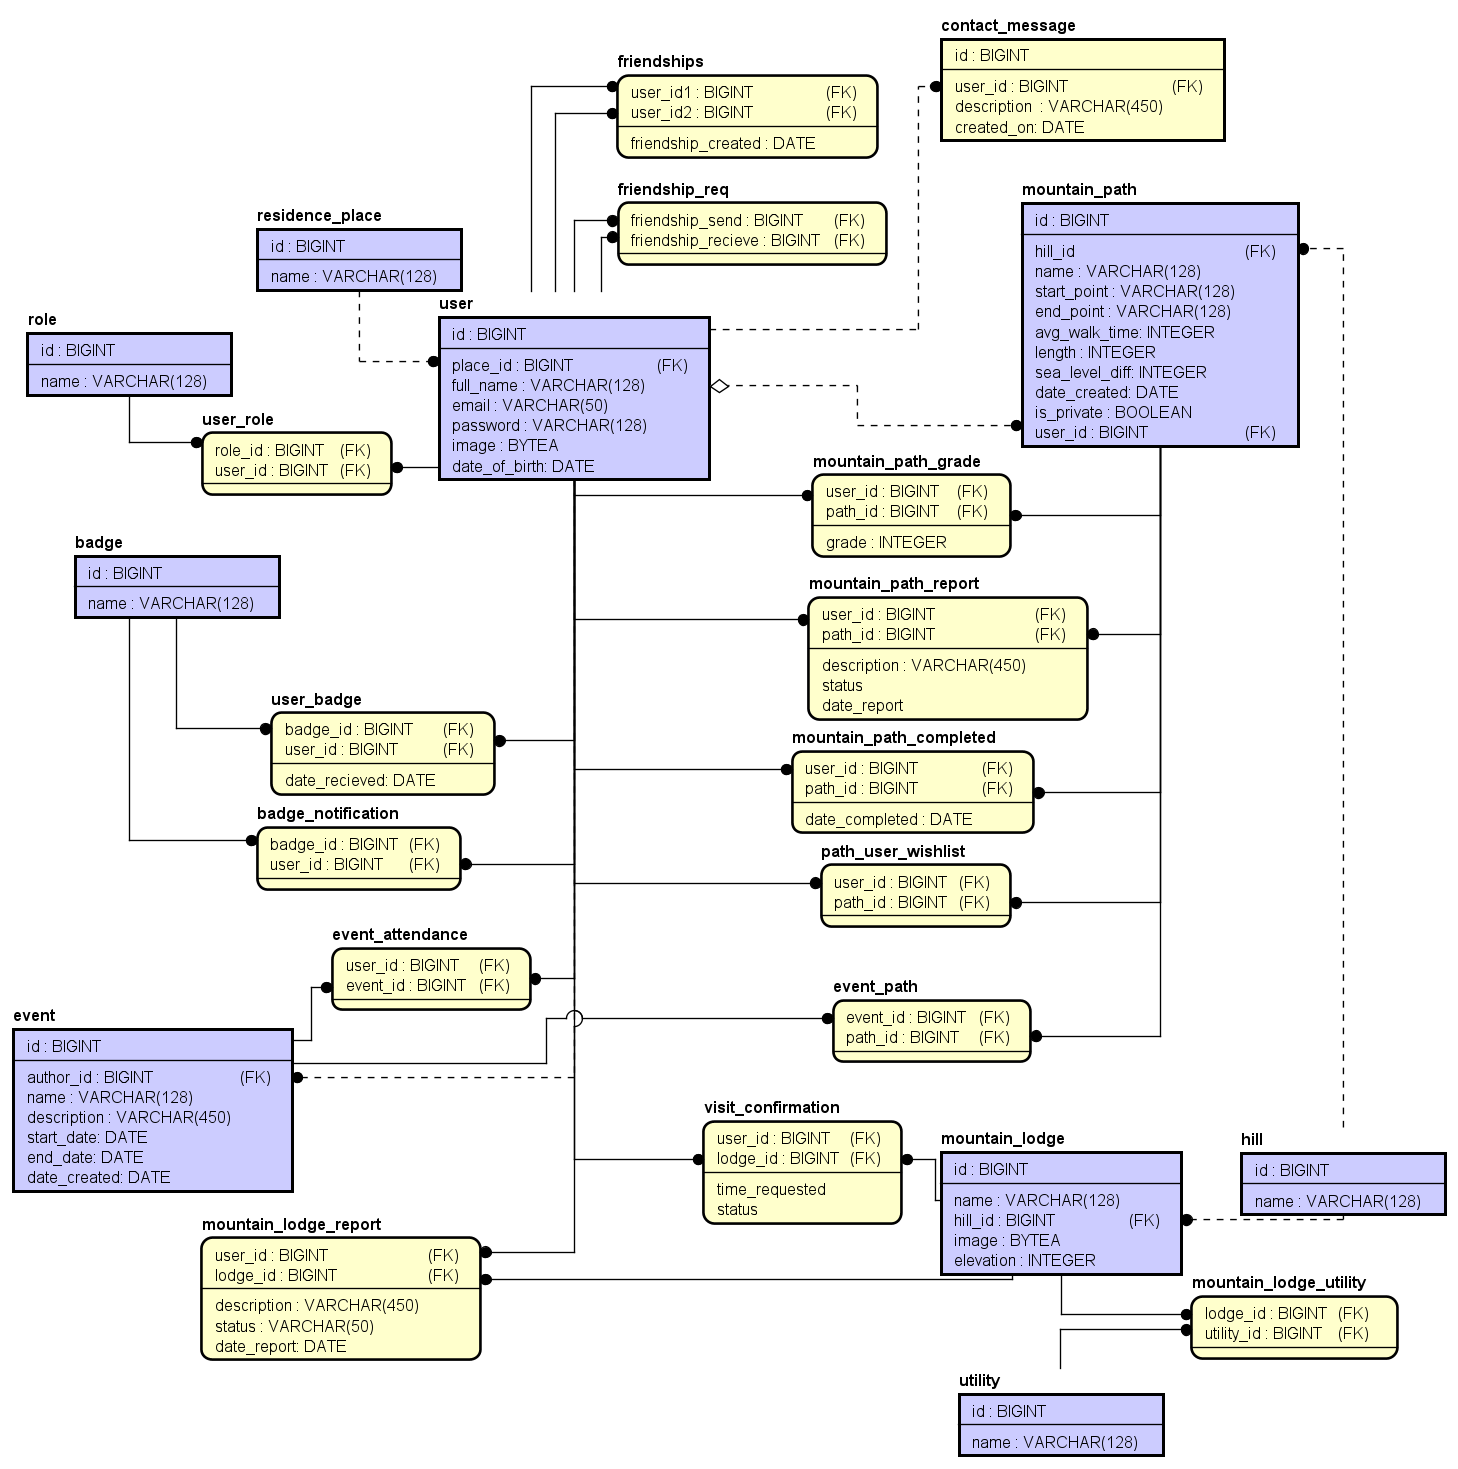
\includegraphics[scale=0.4, height=180mm]{slike/database.png} %veličina slike u odnosu na originalnu datoteku i pozicija slike
					\centering
					\caption{Dijagram baze podataka}
					\label{fig:dijagrambp}
				\end{figure}
			
			\eject
			
			
		\section{Dijagram razreda}
		
			\subsection{Konceptualni model dijagrama razreda}
			Prvi prikazani dijagram je konceptualni model dijagrama razreda. Na njemu su idejno prikazani razredi, njihove funkcionalnosti te odnosi između razreda. Svi razredi napravljeni su obzirom na obrasce uporabe i opise funkcionalnih zahtjeva.
		
			\begin{figure}[H]
				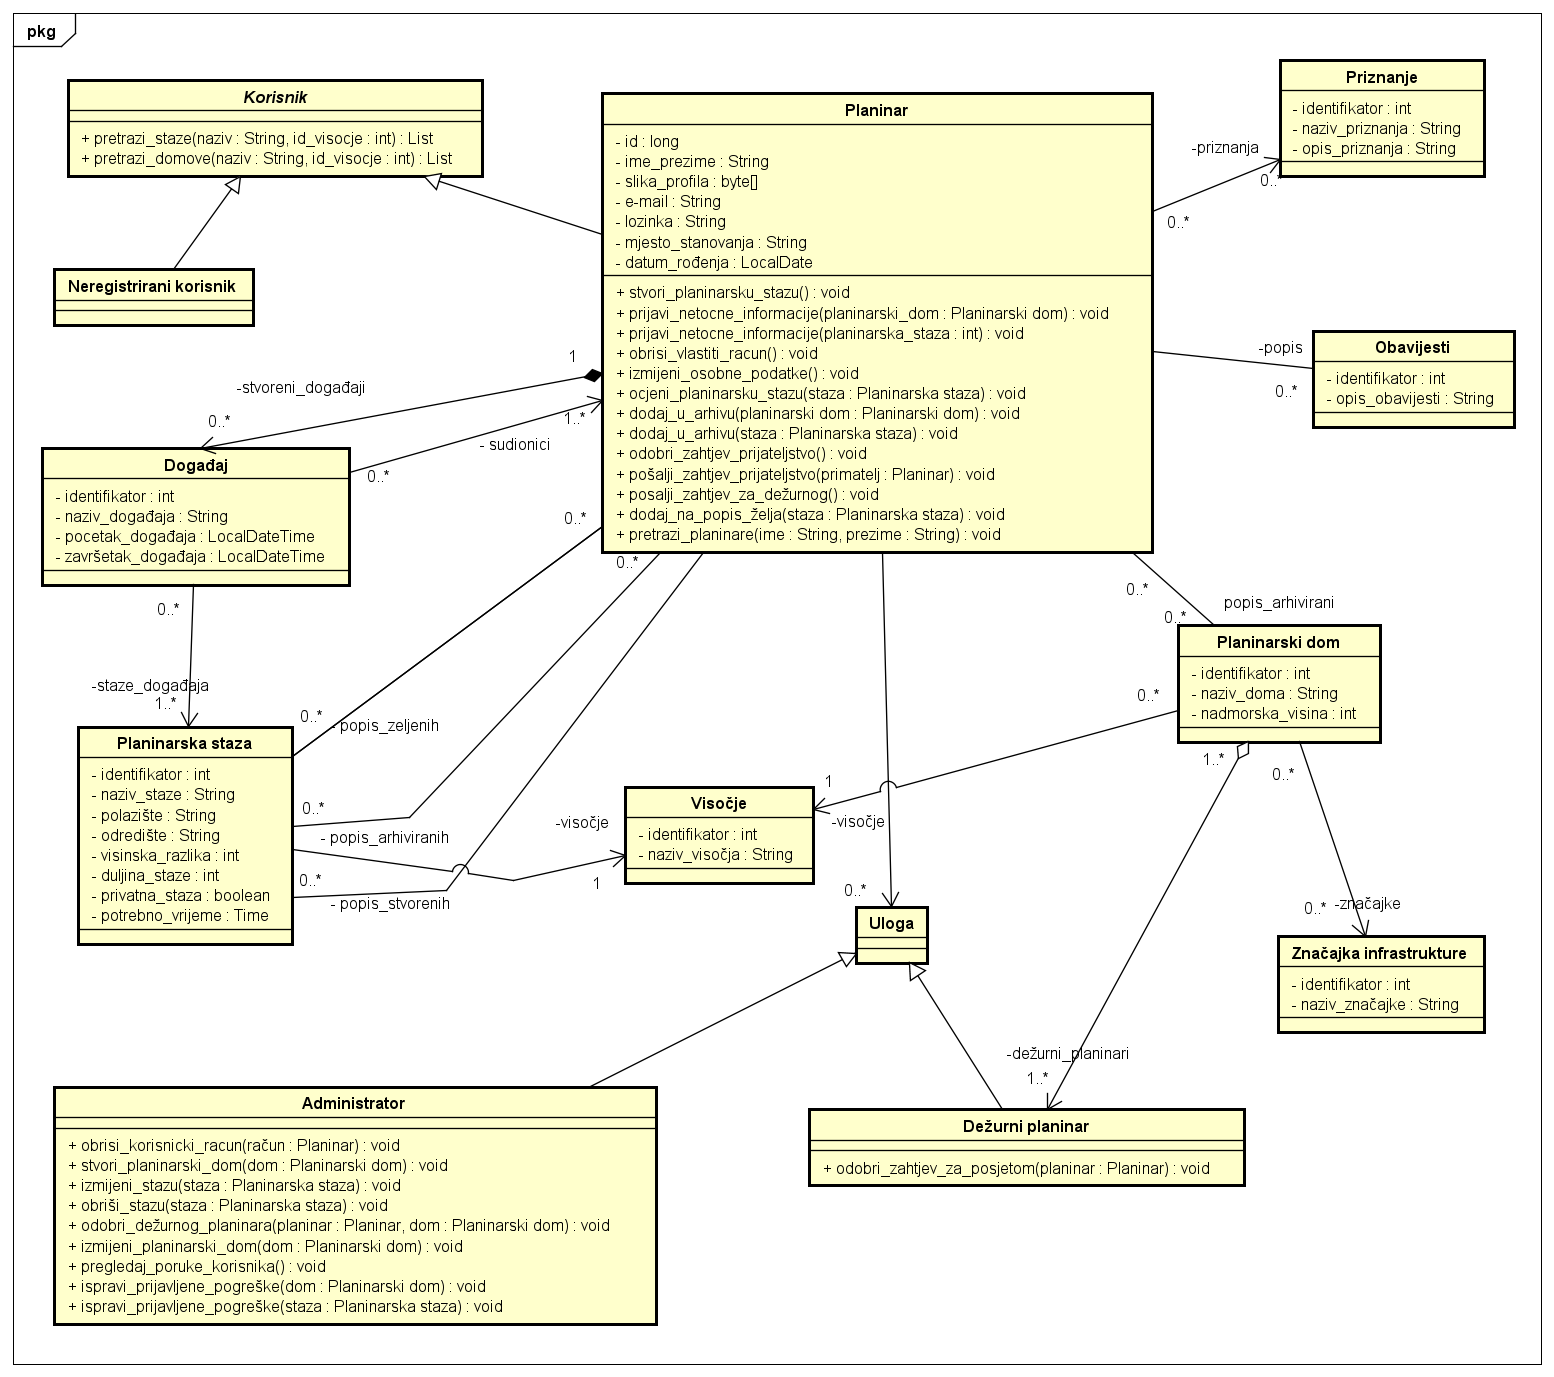
\includegraphics[scale=0.4, height=170mm, width=165mm]{dijagrami/domena-konceptualni.png} %veličina slike u odnosu na originalnu datoteku i pozicija slike
				\centering
				\caption{Dijagram razreda - konceptualni model}
				\label{fig:dijagrami_razreda3}
			\end{figure}
			
			\eject
			
			\subsection{Implementacijski dijagrami razreda - model sustava}
			\subsubsection{Sloj modela i objekti prijenosa podataka (DTO)}
			Na ovom dijagramu prikazan je sloj modela te su prikazani objekti prijenosa podataka, tzv. \textit{Data Transfer Objects}. Ovaj dijagram modela odnosi se na modele sustava koji su trenutno implementirani i koji omogućuju generičke funkcionalnosti potrebne za prvu predaju. U daljnjem radu i razvitku ovaj dijagram će se nadopunjavati sve do konačnog modela sustava. Možemo reći da je glavni razred na dijagramu razred \textit{User}, koji predstavlja registriranog korisnika aplikacije, odnosno planinara. On je povezan s razredom \textit{Role}, na način da svaki korisnik može imati više aplikativnih uloga, npr. ulogu \textit{Admin} ili \textit{Dežurni planinar}, međutim funkcionalnosti vezane uz te uloge još nisu implementirane. Vidimo i razred \textit{MountainLodge} koji modelira jedan planinarski dom. Planinarski dom može imati više značajki infrastrukture, što je na dijagramu prikazano vezom razreda \textit{MountainLodge} s razredom \textit{Utility}. Planinarski dom se isključivo nalazi na jednom visočju, koje je modelirano razredom \textit{Hill}. Osim tih razreda prikazani su DTO razredi: \textit{HillFindResponse}, \textit{UserCreateDto}, \textit{MountainLodgeSearchRequest}, \textit{MountainLodgeSearchResponse} te \textit{PageSearchResponse}. To su razredi koji služe za prijenos podataka i omogućavaju da nadglednik nikada ne radi sa stvarnim modelima. Osim njih, prikazano je sučelje \textit{DefaultMapper} kojeg implementiraju konkretni razredi za mapiranje, čija je dužnost mapirati razrede prijenosa podataka u modele i obrnuto. Za razrede modela prikazane su metode, dok za DTO objekte metode nisu prikazane zbog preglednosti.
			\begin{figure}[H]
				\includegraphics[scale=0.6, height=190mm, width=165mm]{dijagrami/model-DTO-sloj.png} %veličina slike u odnosu na originalnu datoteku i pozicija slike
				\centering
				\caption{Dijagram razreda - sloj modela i DTO}
				\label{fig:dijagrami_razreda2}
			\end{figure}
			\newpage
			\subsubsection{Daljnja idejna razrada sloja modela}
			Na sljedećem dijagramu idejno su prikazani prethodni modeli s novim metodama i razredi koji će se razvijati u narednim iteracijama razvoja projekta. 
			\begin{figure}[H]
				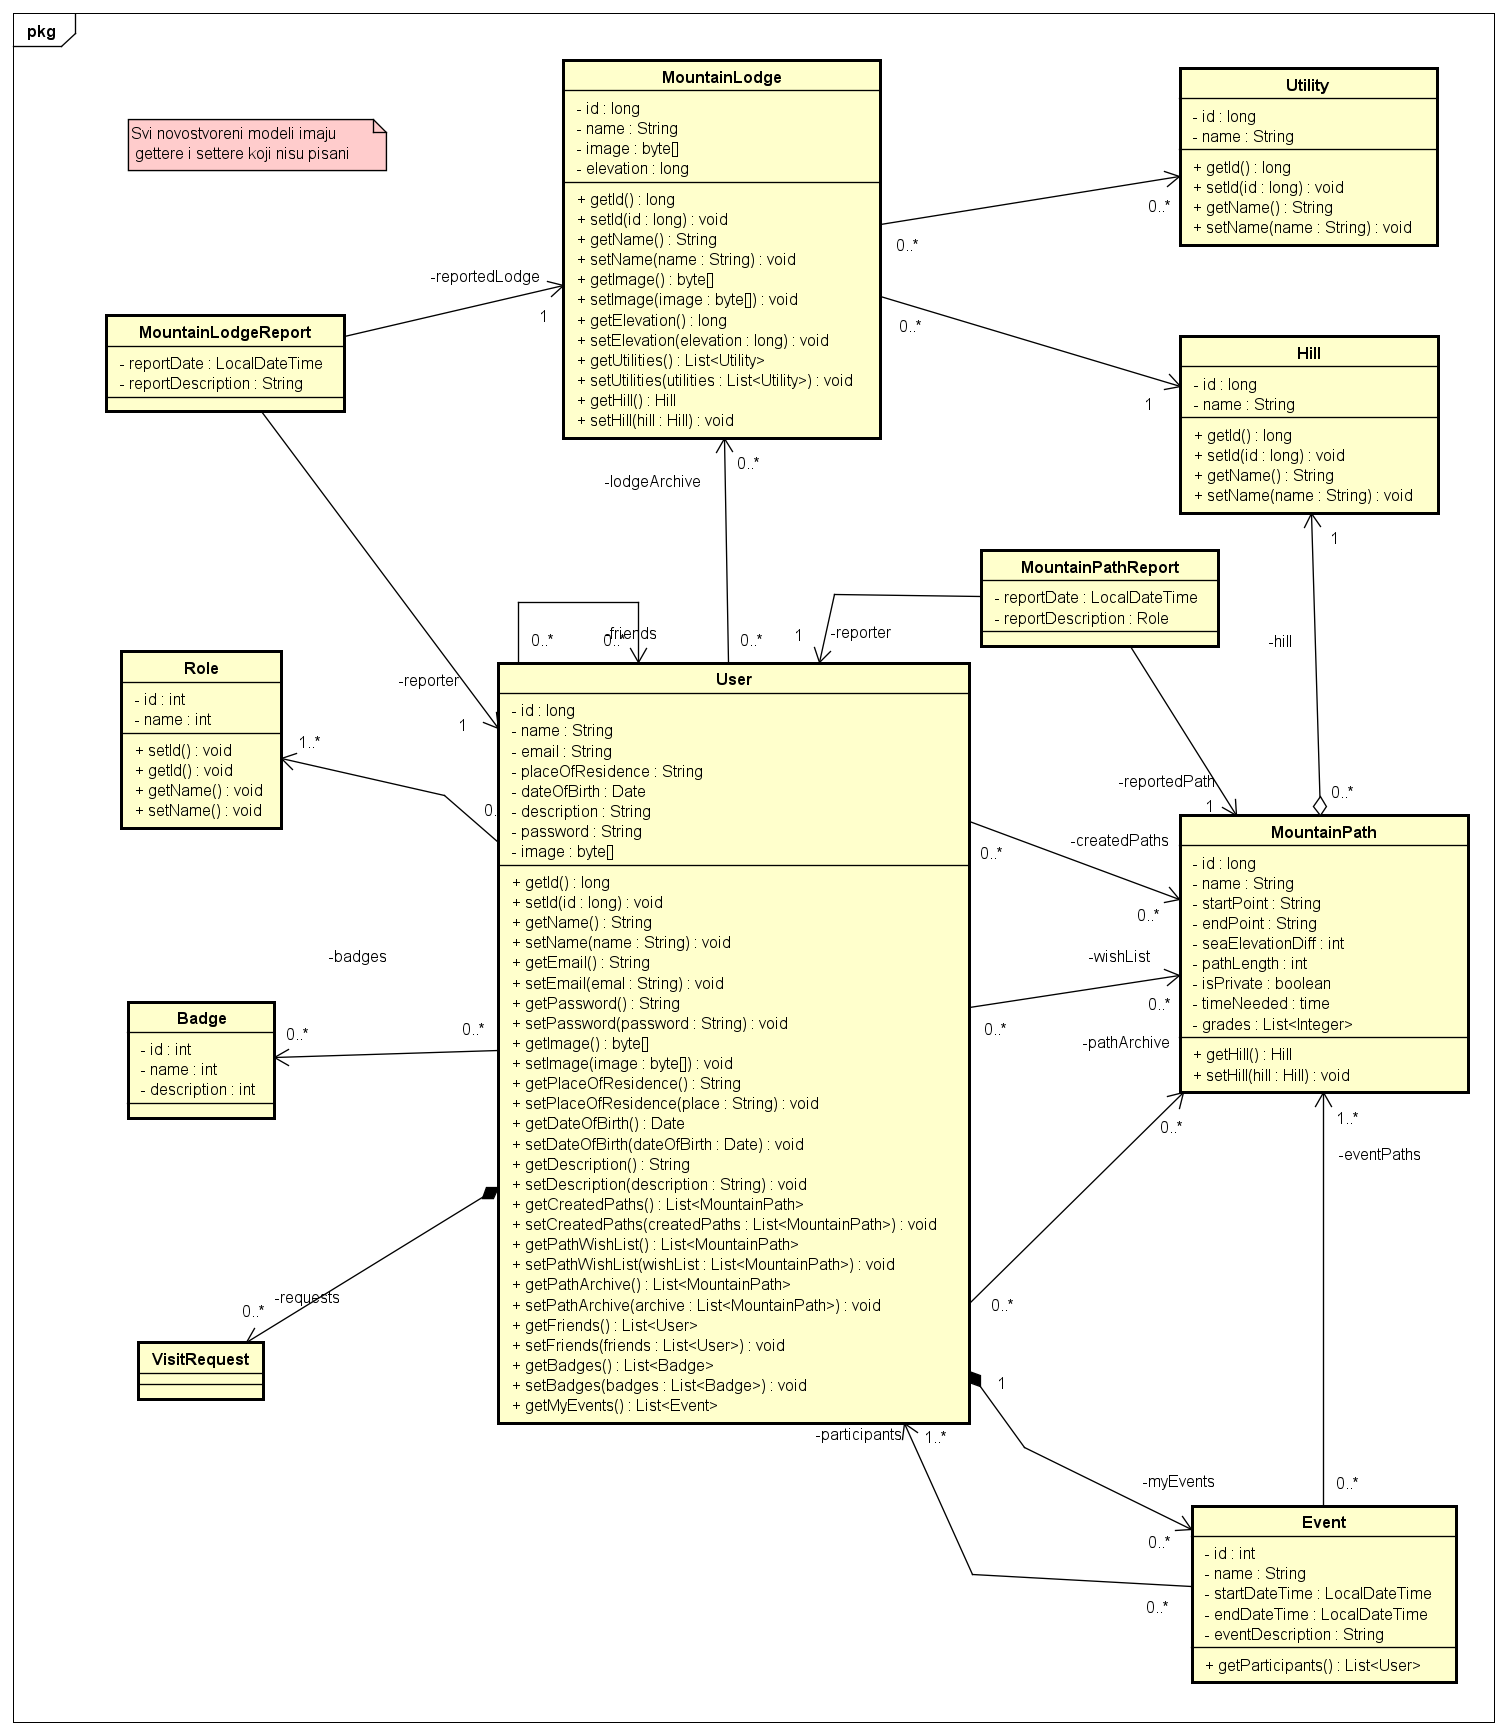
\includegraphics[scale=0.6, height=170mm, width=165mm]{dijagrami/future-model.png} %veličina slike u odnosu na originalnu datoteku i pozicija slike
				\centering
				\caption{Dijagram razreda - idejna razrada daljnjih modela}
				\label{fig:dijagrami_razreda3}
			\end{figure}
			\newpage
			\subsubsection{Sloj nadglednik - servis - repozitorij}
			Ovaj sloj predstavlja sve operacije koje naš sustav obavlja. Razrađen je po oblikovnom obrascu "MVC". Zapravo se ovaj sloj sastoji od tri podsloja, a to su: 
			\begin{itemize}
				\item 
					Sloj repozitorija - metode pristupa bazi podataka, dohvat modela
				\item
					Sloj servisa - tu se obavlja sva naša poslovna logika, pozivaju se metode repozitorija dohvaćaju se podaci
				\item Sloj nadglednika - prima zahtjeve od korisnika i poziva metoda servisnog sloja	
			\end{itemize}
			Razredi koji su trenutno implementirani u ovom sloju prikazani su na dijagramu slijedno, od najnižeg podsloja odnosno pristupa bazi podataka pa sve do podsloja nadglednika koji prima i delegira zahtjeve korisnika.
			Dijagram se sastoji od nekoliko nadglednika: \textit{MountainLodgeController}, \textit{HillController} te \textit{UserController}, a svi su označeni anotacijom \textit{@RestController}. 
			
			Podsloj nadglednika povezan je sa servisnim slojem preko konkretnog primjerka razreda servisnog sloja kojeg čine razredi \textit{MountainLodgeQueryServiceImpl}, \textit{HillQueryServiceImpl} te \textit{UserQueryServiceImpl}, a oni predstavljaju implementacije odgovarajućih servisnih sučelja koji su također označeni na dijagramu.
			
			 Naposljetku, servisni sloj povezan je sa slojem repozitorija preko sučelja konkretnog repozitorija relevantnog za taj servis. U našem slučaju to su sučelja: \textit{MountainLodgeRepository}, \textit{HillRepository} te \textit{UserRepository}. Svako sučelje repozitorija nasljeđuje sučelje \textit{JpaRepository} koje sadrži konkretnu implementaciju upita nad bazom podataka.
			 
			  Sučelje \textit{JpaSpecificationExecutor} omogućuje nam korištenje specifikacije \textit{MountainLodgeSearchSpecification} prilikom pretraživanja planinarskih domova iz baze podataka.
			\begin{figure}[H]
				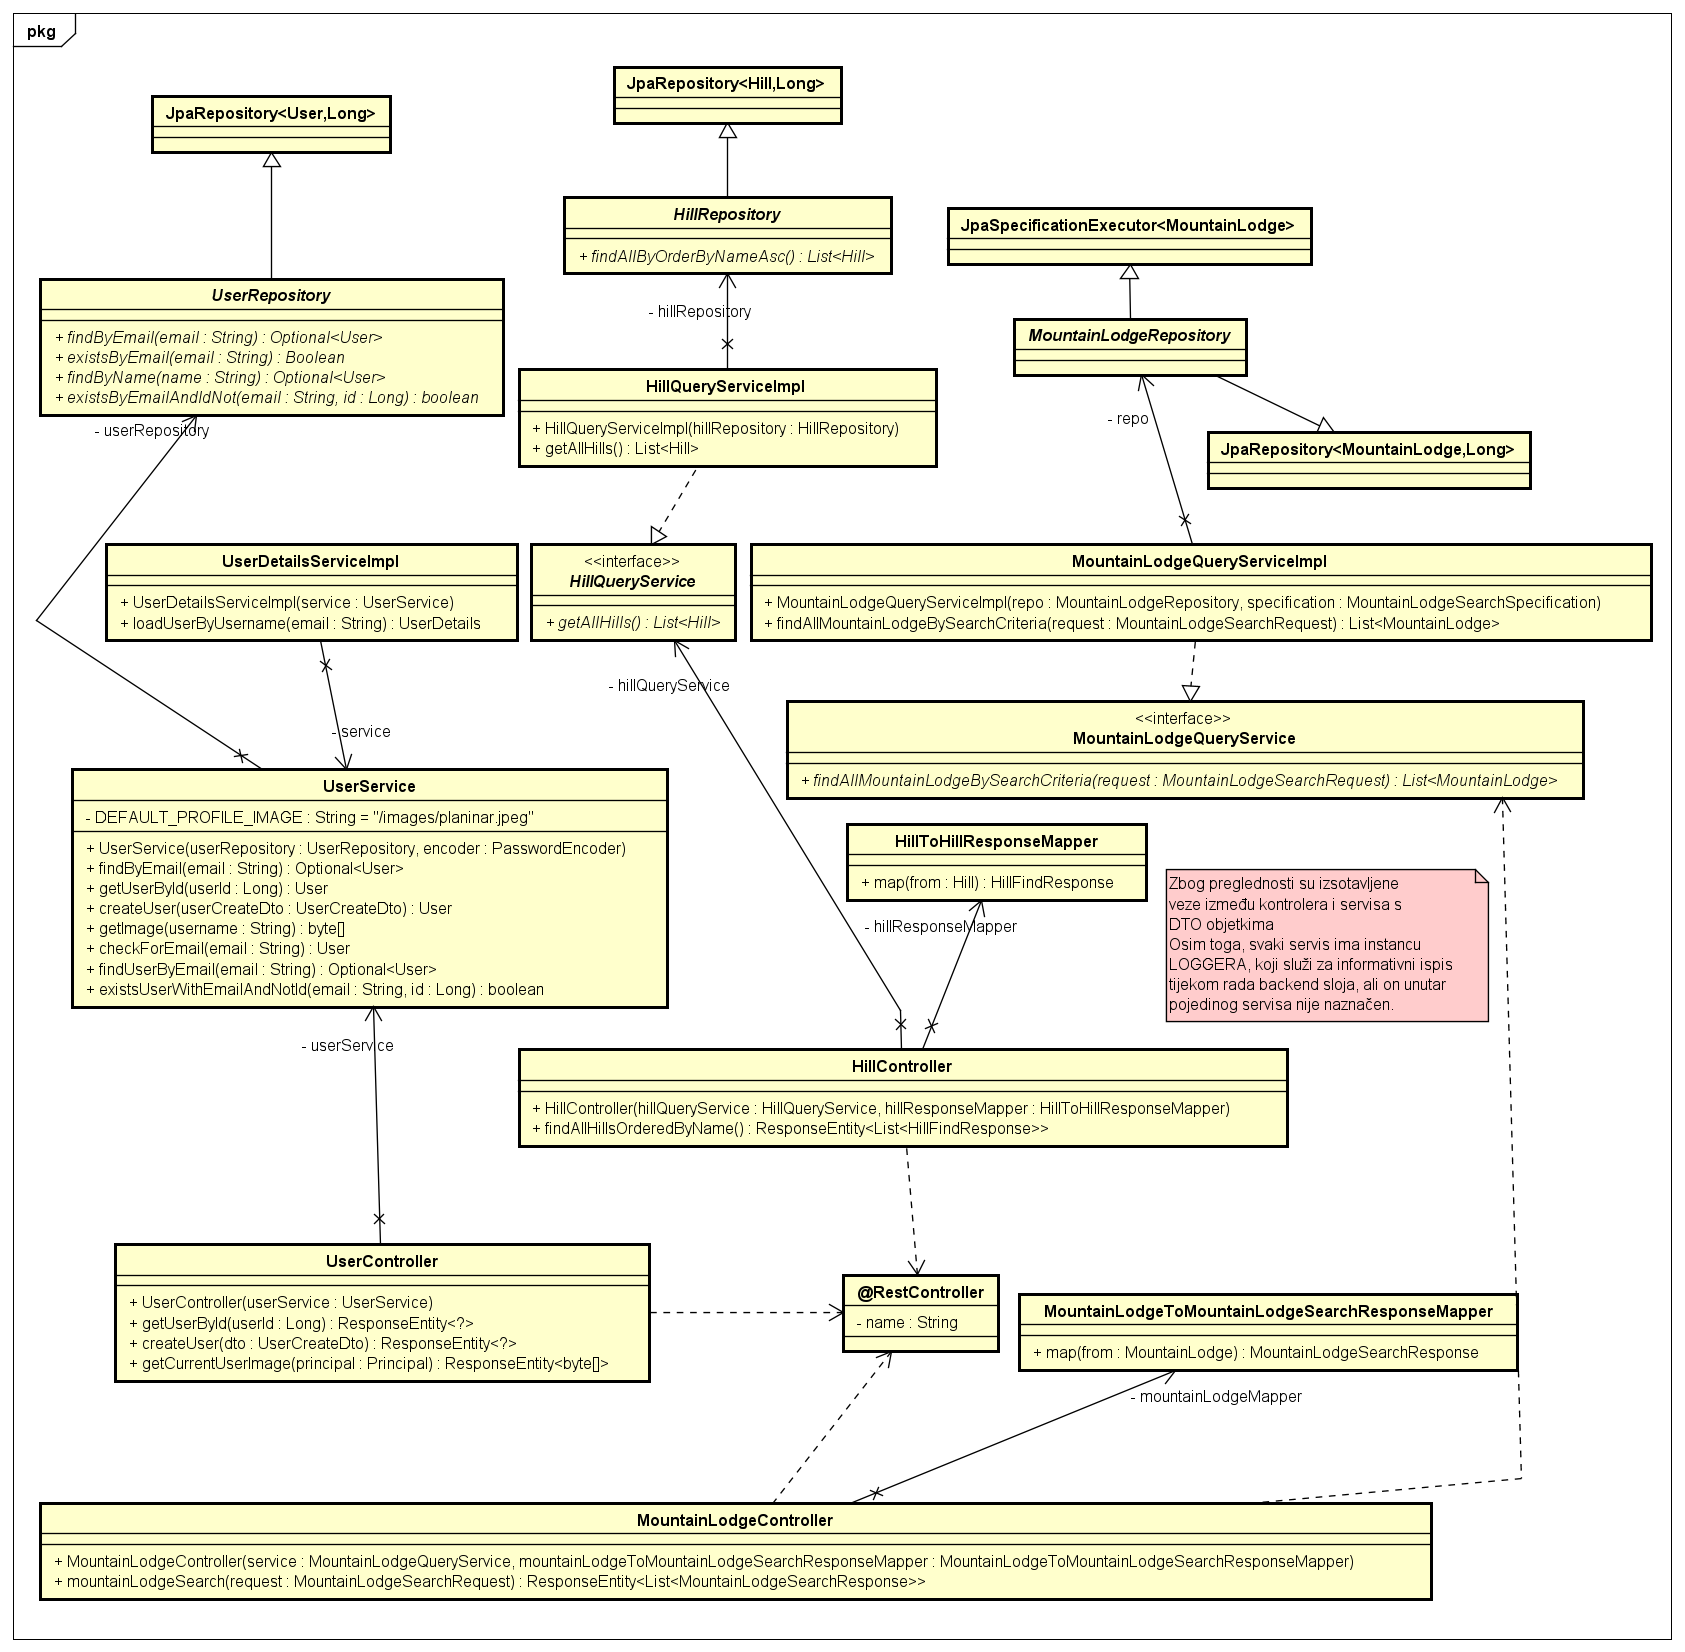
\includegraphics[scale=0.6, height=175mm, width=165mm]{dijagrami/rest.png} %veličina slike u odnosu na originalnu datoteku i pozicija slike
				\centering
				\caption{Dijagram razreda - sloj nadglednik - servis - repozitorij}
				\label{fig:dijagrami_razreda4}
			\end{figure}
			\newpage
			\subsubsection{Razredi vezani uz sigurnost i pomoćni razredi}
			Prilikom prijave korisnika, zahtjev za prijavu se šalje na back end, točnije do nadglednika. Zahtjev se provjerava u razredu \textit{JWTAuthenticationFilter} pomoću metode \textit{attemptAuthentication} koja stvara instancu razreda \textit{UserLogin} i šalje ga na provjeru.
			 
			 Provjera se vrši tako da se zove metoda \textit{loadUserByUsername} razreda \textit{UserDetailsServiceImpl}, a ona provjerava postoji li korisnik koji sadrži e-mail koji je poslan unutar zahtjeva. 
			 
			 Nakon utvrđivanja da ta osoba postoji \textit{Spring security modul} provjerava lozinku i druge podatke vezane uz prijavu. Nakon uspješne prijave pomoću metode \textit{successfulAuthentication} se generira jedinstveni token (identifikator) i šalje korisniku. Svojstva tokena poput trajanja se određuju u razredu \textit{SecurityConstants}. 
			
			Prijavljeni korisnik za vrijeme rada unutar Web aplikacije svaki zahtjev obavlja pomoću jedinstvenog tokena koji mu je dodijeljen, a koji se provjerava unutar razreda \textit{JWTAuthorizationFilter}. 
			
			Metoda \textit{getPasswordEncoder} razreda \textit{Configuration} služi da bi definirali enkoder za zaštitu lozinki. 
			
			Razred \textit{UniqueEmailValidator} prilikom registracije provjerava postoji li u bazi podataka korisnik kojem je e-mail isti e-mailu zahtjeva. Budući da ne možemo imati dva korisnika s istom adresom elektroničke pošte, u tom slučaju događa se iznimka \textit{UserWithEmailExistsException}.  
			
			Razredi \textit{NoImageException} i \textit{ResourceNotFoundException} modeliraju iznimke koje se mogu dogoditi prilikom rada sustava.
			Razred \textit{MountainLodgeSearchSpecification} koji je konkretna implementacija parametriziranog sučelja \textit{BaseSpecification} omogućava nam pretraživanje planinarskih domova prema određenim kriterijima.
			
		
			\begin{figure}[H]
				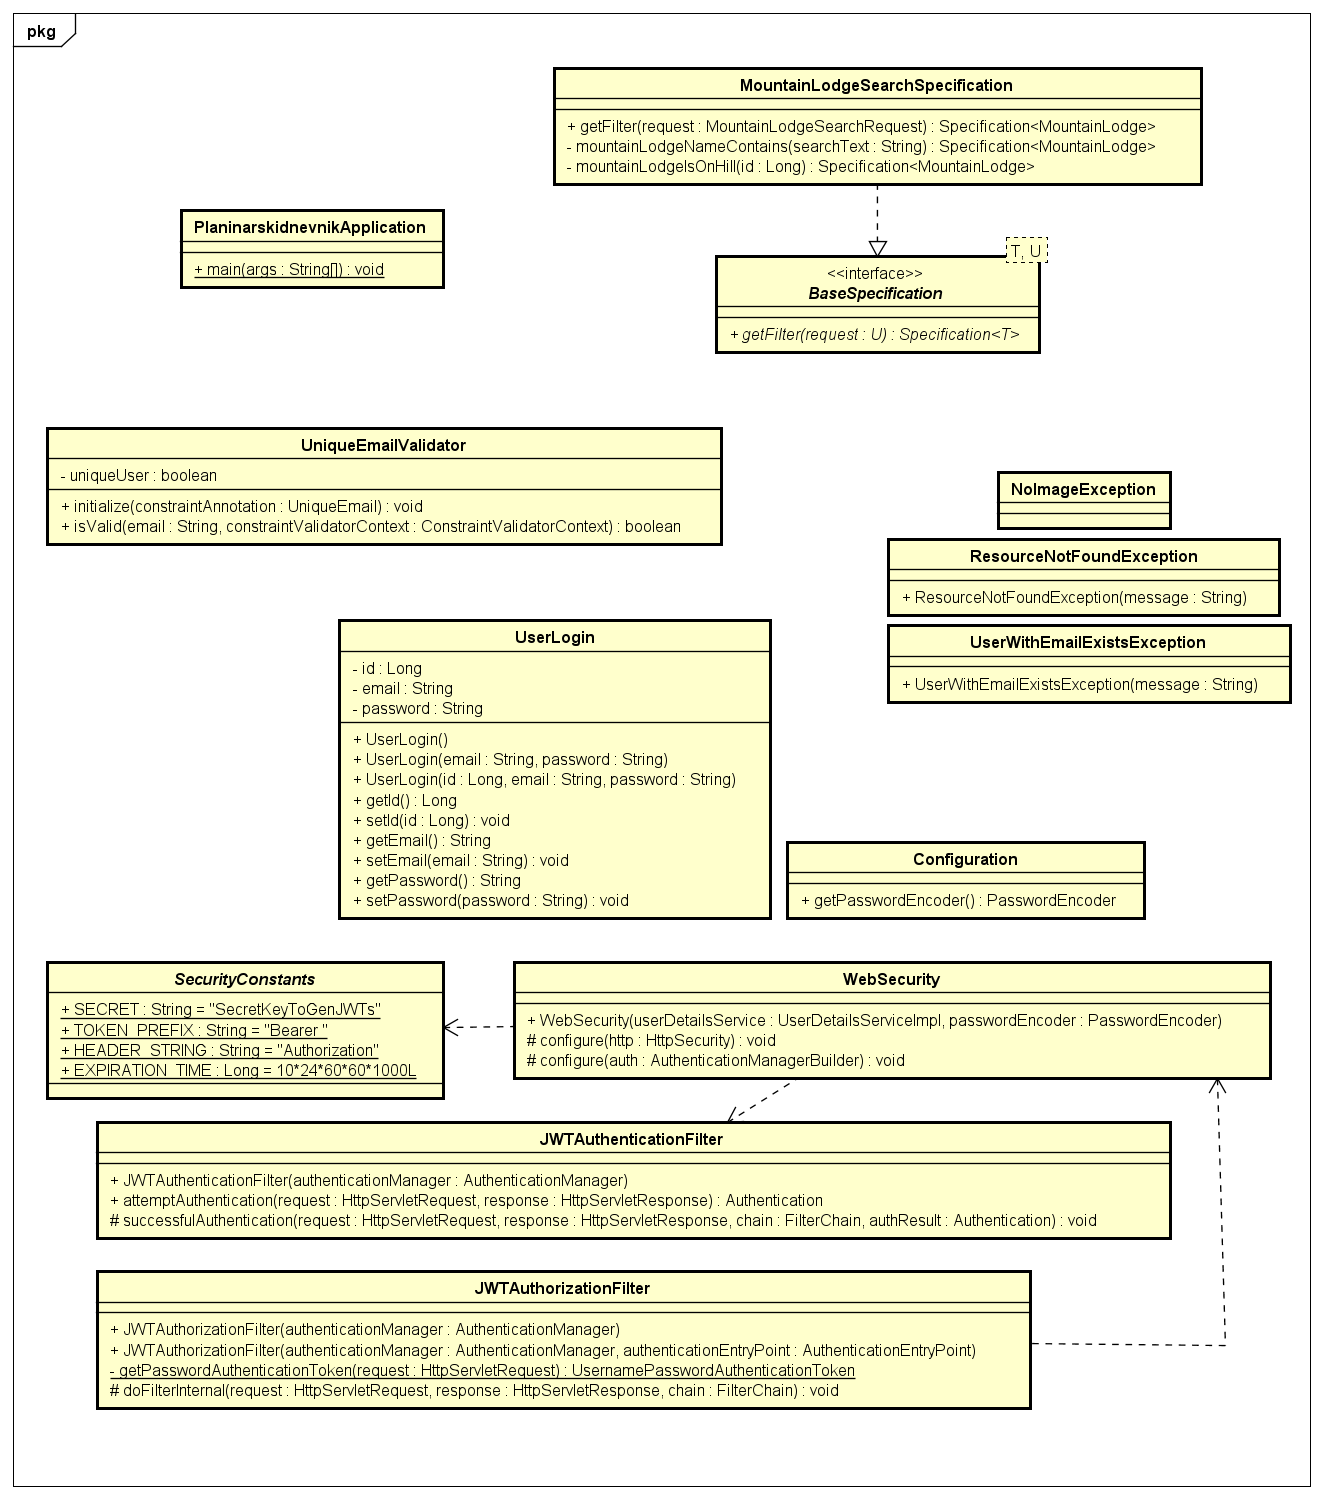
\includegraphics[scale=0.6, height=175mm, width=165mm]{dijagrami/helpers-class.png} %veličina slike u odnosu na originalnu datoteku i pozicija slike
				\centering
				\caption{Dijagram razreda - sigurnost i pomoćne metode}
				\label{fig:dijagrami_razreda5}
			\end{figure}
			
			\eject
			
			
			
			
			\eject
		
		%\section{Dijagram stanja}
			
			
		%	\textbf{\textit{dio 2. revizije}}\\
		%	
		%	\textit{Potrebno je priložiti dijagram stanja i opisati ga. Dovoljan je jedan dijagram stanja koji prikazuje \textbf{značajan dio funkcionalnosti} sustava. Na primjer, stanja korisničkog sučelja i tijek korištenja neke ključne funkcionalnosti jesu značajan dio sustava, a registracija i prijava nisu. }
			
			
		%	\eject 
		
		%\section{Dijagram aktivnosti}
		%	
		%	\textbf{\textit{dio 2. revizije}}\\
			
		%	 \textit{Potrebno je priložiti dijagram aktivnosti s pripadajućim opisom. Dijagram aktivnosti treba prikazivati značajan dio sustava.}
			
		%	\eject
		%\section{Dijagram komponenti}
		
		%	\textbf{\textit{dio 2. revizije}}\\
		
		%	 \textit{Potrebno je priložiti dijagram komponenti s pripadajućim opisom. Dijagram komponenti treba prikazivati strukturu cijele aplikacije.}
	%\chapter{Implementacija i korisničko sučelje}
		
		
		\section{Korištene tehnologije i alati}
		
			\textbf{\textit{dio 2. revizije}}
			
			 \textit{Detaljno navesti sve tehnologije i alate koji su primijenjeni pri izradi dokumentacije i aplikacije. Ukratko ih opisati, te navesti njihovo značenje i mjesto primjene. Za svaki navedeni alat i tehnologiju je potrebno \textbf{navesti internet poveznicu} gdje se mogu preuzeti ili više saznati o njima}.
			
			
			\eject 
		
	
		\section{Ispitivanje programskog rješenja}
			
			\textbf{\textit{dio 2. revizije}}\\
			
			 \textit{U ovom poglavlju je potrebno opisati provedbu ispitivanja implementiranih funkcionalnosti na razini komponenti i na razini cijelog sustava s prikazom odabranih ispitnih slučajeva. Studenti trebaju ispitati temeljnu funkcionalnost i rubne uvjete.}
	
			
			\subsection{Ispitivanje komponenti}
			\textit{Potrebno je provesti ispitivanje jedinica (engl. unit testing) nad razredima koji implementiraju temeljne funkcionalnosti. Razraditi \textbf{minimalno 6 ispitnih slučajeva} u kojima će se ispitati redovni slučajevi, rubni uvjeti te izazivanje pogreške (engl. exception throwing). Poželjno je stvoriti i ispitni slučaj koji koristi funkcionalnosti koje nisu implementirane. Potrebno je priložiti izvorni kôd svih ispitnih slučajeva te prikaz rezultata izvođenja ispita u razvojnom okruženju (prolaz/pad ispita). }
			
			
			
			\subsection{Ispitivanje sustava}
			
			 \textit{Potrebno je provesti i opisati ispitivanje sustava koristeći radni okvir Selenium\footnote{\url{https://www.seleniumhq.org/}}. Razraditi \textbf{minimalno 4 ispitna slučaja} u kojima će se ispitati redovni slučajevi, rubni uvjeti te poziv funkcionalnosti koja nije implementirana/izaziva pogrešku kako bi se vidjelo na koji način sustav reagira kada nešto nije u potpunosti ostvareno. Ispitni slučaj se treba sastojati od ulaza (npr. korisničko ime i lozinka), očekivanog izlaza ili rezultata, koraka ispitivanja i dobivenog izlaza ili rezultata.\\ }
			 
			 \textit{Izradu ispitnih slučajeva pomoću radnog okvira Selenium moguće je provesti pomoću jednog od sljedeća dva alata:}
			 \begin{itemize}
			 	\item \textit{dodatak za preglednik \textbf{Selenium IDE} - snimanje korisnikovih akcija radi automatskog ponavljanja ispita	}
			 	\item \textit{\textbf{Selenium WebDriver} - podrška za pisanje ispita u jezicima Java, C\#, PHP koristeći posebno programsko sučelje.}
			 \end{itemize}
		 	\textit{Detalji o korištenju alata Selenium bit će prikazani na posebnom predavanju tijekom semestra.}
			
			\eject 
		
		
		\section{Dijagram razmještaja}
			
			\textbf{\textit{dio 2. revizije}}
			
			 \textit{Potrebno je umetnuti \textbf{specifikacijski} dijagram razmještaja i opisati ga. Moguće je umjesto specifikacijskog dijagrama razmještaja umetnuti dijagram razmještaja instanci, pod uvjetom da taj dijagram bolje opisuje neki važniji dio sustava.}
			
			\eject 
		
		\section{Upute za puštanje u pogon}
		
			\textbf{\textit{dio 2. revizije}}\\
		
			 \textit{U ovom poglavlju potrebno je dati upute za puštanje u pogon (engl. deployment) ostvarene aplikacije. Na primjer, za web aplikacije, opisati postupak kojim se od izvornog kôda dolazi do potpuno postavljene baze podataka i poslužitelja koji odgovara na upite korisnika. Za mobilnu aplikaciju, postupak kojim se aplikacija izgradi, te postavi na neku od trgovina. Za stolnu (engl. desktop) aplikaciju, postupak kojim se aplikacija instalira na računalo. Ukoliko mobilne i stolne aplikacije komuniciraju s poslužiteljem i/ili bazom podataka, opisati i postupak njihovog postavljanja. Pri izradi uputa preporučuje se \textbf{naglasiti korake instalacije uporabom natuknica} te koristiti što je više moguće \textbf{slike ekrana} (engl. screenshots) kako bi upute bile jasne i jednostavne za slijediti.}
			
			
			 \textit{Dovršenu aplikaciju potrebno je pokrenuti na javno dostupnom poslužitelju. Studentima se preporuča korištenje neke od sljedećih besplatnih usluga: \href{https://aws.amazon.com/}{Amazon AWS}, \href{https://azure.microsoft.com/en-us/}{Microsoft Azure} ili \href{https://www.heroku.com/}{Heroku}. Mobilne aplikacije trebaju biti objavljene na F-Droid, Google Play ili Amazon App trgovini.}
			
			
			\eject 
	%\chapter{Zaključak i budući rad}
		
		\textbf{\textit{dio 2. revizije}}\\
		
		 \textit{U ovom poglavlju potrebno je napisati osvrt na vrijeme izrade projektnog zadatka, koji su tehnički izazovi prepoznati, jesu li riješeni ili kako bi mogli biti riješeni, koja su znanja stečena pri izradi projekta, koja bi znanja bila posebno potrebna za brže i kvalitetnije ostvarenje projekta i koje bi bile perspektive za nastavak rada u projektnoj grupi.}
		
		 \textit{Potrebno je točno popisati funkcionalnosti koje nisu implementirane u ostvarenoj aplikaciji.}
		
		\eject 
	\chapter*{Popis literature}
		\addcontentsline{toc}{chapter}{Popis literature}
	 	
		
		\begin{enumerate}
			
			
			\item  Programsko inženjerstvo, FER ZEMRIS, \url{http://www.fer.hr/predmet/proinz}
			
			\item  I. Sommerville, "Software engineering", 8th ed, Addison Wesley, 2007.
			
			\item  T.C.Lethbridge, R.Langaniere, "Object-Oriented Software Engineering", 2nd ed. McGraw-Hill, 2005.
			
			\item  I. Marsic, Software engineering book``, Department of Electrical and Computer Engineering, Rutgers University, \url{http://www.ece.rutgers.edu/~marsic/books/SE}
			
			\item  The Unified Modeling Language, \url{https://www.uml-diagrams.org/}
			
			\item  Astah Community, \url{http://astah.net/editions/uml-new}
		\end{enumerate}
		
		 
	
	
	\begingroup
	\renewcommand*\listfigurename{Indeks slika i dijagrama}
	%\renewcommand*\listtablename{Indeks tablica}
	%\let\clearpage\relax
	\listoffigures
	%\vspace{10mm}
	%\listoftables
	\endgroup
	\addcontentsline{toc}{chapter}{Indeks slika i dijagrama}


	
	\eject 
		
	\chapter*{Dodatak: Prikaz aktivnosti grupe}
		\addcontentsline{toc}{chapter}{Dodatak: Prikaz aktivnosti grupe}
		
		\section*{Dnevnik sastajanja}
		
		\begin{packed_enum}
			\item  sastanak
			
			\item[] \begin{packed_item}
				\item Datum:  7. listopada 2020.
				\item Prisustvovali: I.Martinović, M.Rajnović, N.Kušurin, H.Ladić, L.Ravenšćak, J.Kaselj, D.Konjevod
				\item Teme sastanka: 
				\begin{packed_item}
					\item  Komentiranje zadatka koji smo dobili i komentiranje nejasnih dijelova
					\item  Razgovor o poznavanju tehnologija (Git, Spring, React)
					\item  Dogovor o tutorialima koje treba pogledati na internetu
					\item  Razgovor o funkcioniranju platforme Gitlab
				\end{packed_item}
			\end{packed_item}
			
			\item  sastanak
			\item[] \begin{packed_item}
				\item Datum:  8.listopada 2020.
				\item Prisustvovali: I.Martinović, M.Rajnović, N.Kušurin, H.Ladić, L.Ravenšćak, J.Kaselj, D.Konjevod, K.Labor, M.Bićanić, H.Šimić
				\item Teme sastanka:
				\begin{packed_item}
					\item   Predstavljanje načina rada i uvod u projekt
					\item   Rješavanje nejasnoća vezanih uz zadatak s asistentom i demonstratorom
				\end{packed_item}
			\end{packed_item}
		
			\item  sastanak
			\item[] \begin{packed_item}
				\item Datum:  9.listopada 2020.
				\item Prisustvovali: I.Martinović, M.Rajnović, N.Kušurin, H.Ladić, L.Ravenšćak, J.Kaselj, D.Konjevod
				\item Teme sastanka:
				\begin{packed_item}
					\item   Inicijalizacija projekta (back end i front end) na Gitlabu
					\item   Dogovor oko raspodjele poslova vezanih uz dokumentaciju
				\end{packed_item}
			\end{packed_item}
	
			\item sastanak
			\item[] \begin{packed_item}
				\item Datum: 11.listopada 2020.
				\item Prisustvovali: I.Martinović, M.Rajnović, J.Kaselj
				\item Teme sastanka:
				\begin{packed_item}
					\item   Izlučivanje funkcionalnih zahtjeva
				\end{packed_item}
			\end{packed_item}
		
			\item sastanak
			\item[] \begin{packed_item}
				\item Datum: 11.listopada 2020.
				\item Prisustvovali: N.Kušurin, D.Konjevod, H.Ladić
				\item Teme sastanka:
				\begin{packed_item}
					\item   Opis projektnog zadatka
				\end{packed_item}
			\end{packed_item}
		
		\item sastanak
		\item[] \begin{packed_item}
			\item Datum:  15.listopada 2020.
			\item Prisustvovali: N.Kušurin, D.Konjevod, H.Ladić, I.Martinović, M.Rajnović, J.Kaselj, L.Ravenšćak,  K.Labor
			\item Teme sastanka: 
			\begin{packed_item}
				\item   Raspravljanje o funkcionalnim zahtjevima s asistentom
				\item 	Dogovori za buduću komunikaciju
			\end{packed_item}
		\end{packed_item}
	
	\item sastanak
	\item[] \begin{packed_item}
		\item Datum: 15.listopada 2020.
		\item Prisustvovali: N.Kušurin, D.Konjevod, H.Ladić, I.Martinović, M.Rajnović, J.Kaselj, L.Ravenšćak
		\item Teme sastanka: 
		\begin{packed_item}
			\item   Crtanje ekrana
			\item 	Raspodjela daljnjih poslova
		\end{packed_item}
	\end{packed_item}

	\item sastanak
	\item[] \begin{packed_item}
		\item Datum:  19.listopada 2020.
		\item Prisustvovali: N.Kušurin, D.Konjevod
		\item Teme sastanka: 
		\begin{packed_item}
			\item   Scenariji obrazaca uporabe
		\end{packed_item}
	\end{packed_item}
	
	
	\item sastanak
	\item[] \begin{packed_item}
		\item Datum: 20.listopada 2020.
		\item Prisustvovali: I.Martinović, M.Rajnović, L.Ravenšćak
		\item Teme sastanka: 
		\begin{packed_item}
			\item   Modeliranje baze podataka
		\end{packed_item}
	\end{packed_item}
			
			
			\item sastanak
			\item[] \begin{packed_item}
				\item Datum: 22.listopada 2020.
				\item Prisustvovali: I.Martinović, M.Rajnović, L.Ravenšćak, J.Kaselj, H.Ladić, D.Konjevod, N.Kušurin, K.Labor, M.Bićanić
				\item Teme sastanka: 
				\begin{packed_item}
					\item   Pregledavanje dokumentacije i upute za nastavak s asistentom i demonstratorom
				\end{packed_item}
			\end{packed_item}
			
			
			\item sastanak
			\item[] \begin{packed_item}
				\item Datum: 23.listopada 2020.
				\item Prisustvovali: I.Martinović, J.Kaselj, H.Ladić
				\item Teme sastanka: 
				\begin{packed_item}
					\item   Razrada sekvencijskih dijagrama
				\end{packed_item}
			\end{packed_item}

                         \item sastanak
			\item[] \begin{packed_item}
				\item Datum: 27.listopada 2020.
				\item Prisustvovali: I.Martinović, M.Rajnović, L.Ravenšćak, J.Kaselj, H.Ladić, D.Konjevod, N.Kušurin
				\item Teme sastanka: 
				\begin{packed_item}
					\item   Pokazivanje Gitlaba , sekvencijski dijagrami
				\end{packed_item}
			\end{packed_item}
			
			\item sastanak
			\item[] \begin{packed_item}
				\item Datum: 29.listopada 2020.
				\item Prisustvovali: I.Martinović, M.Rajnović, L.Ravenšćak, J.Kaselj, H.Ladić, D.Konjevod, N.Kušurin, K.Labor, M.Bićanić
				\item Teme sastanka: 
				\begin{packed_item}
					\item   Sastanak s asistentom, komentari na sekvencijske dijagrame i dijagrame obrazaca uporabe
				\end{packed_item}
			\end{packed_item}
		\item sastanak
		\item[] \begin{packed_item}
			\item Datum: 5.studenog 2020.
			\item Prisustvovali: I.Martinović, M.Rajnović, L.Ravenšćak, J.Kaselj, H.Ladić, D.Konjevod, N.Kušurin, K.Labor, M.Bićanić
			\item Teme sastanka: 
			\begin{packed_item}
				\item   Sastanak s asistentom i demonstratorom, upute za daljnji rad i razvoj, demonstracija napravljenog i dogovor za predaju
			\end{packed_item}
		\end{packed_item}
	\item sastanak
	\item[] \begin{packed_item}
		\item Datum: 12.studenog 2020.
		\item Prisustvovali: I.Martinović, M.Rajnović, L.Ravenšćak, J.Kaselj, H.Ladić, D.Konjevod, N.Kušurin, K.Labor, M.Bićanić, H.Šimić
		\item Teme sastanka: 
		\begin{packed_item}
			\item   Demonstracija generičkih funkcionalnosti
		\end{packed_item}
	\end{packed_item}
			
			%
			
		\end{packed_enum}
		
			
		\eject
		\section*{Tablica aktivnosti}
		
			
			\begin{longtabu} to \textwidth {|X[7, l]|X[1, c]|X[1, c]|X[1, c]|X[1, c]|X[1, c]|X[1, c]|X[1, c]|}
								
				\cline{2-8} \multicolumn{1}{c|}{\textbf{}} &     \multicolumn{1}{c|}{\rotatebox{90}{\textbf{Ivan Martinović }}} & 
				\multicolumn{1}{c|}{\rotatebox{90}{\textbf{Luka Ravenšćak }}} &	\multicolumn{1}{c|}{\rotatebox{90}{\textbf{Marko Rajnović}}} &	\multicolumn{1}{c|}{\rotatebox{90}{\textbf{Josipa Kaselj}}} &
				\multicolumn{1}{c|}{\rotatebox{90}{\textbf{Neda Kušurin}}} &
				\multicolumn{1}{c|}{\rotatebox{90}{\textbf{Helena Ladić}}} &	\multicolumn{1}{c|}{\rotatebox{90}{\textbf{David Konjevod}}} \\ \hline 
				\endfirsthead
				
			
				\cline{2-8} \multicolumn{1}{c|}{\textbf{}} &     \multicolumn{1}{c|}{\rotatebox{90}{\textbf{Ivan Martinović }}} & 
				\multicolumn{1}{c|}{\rotatebox{90}{\textbf{Luka Ravenšćak }}} &	\multicolumn{1}{c|}{\rotatebox{90}{\textbf{Marko Rajnović}}} &	\multicolumn{1}{c|}{\rotatebox{90}{\textbf{Josipa Kaselj}}} &
				\multicolumn{1}{c|}{\rotatebox{90}{\textbf{Neda Kušurin}}} &
				\multicolumn{1}{c|}{\rotatebox{90}{\textbf{Helena Ladić}}} &	\multicolumn{1}{c|}{\rotatebox{90}{\textbf{David Konjevod}}} \\ \hline  
				\endhead
				
				
				\endfoot
							
				 
				\endlastfoot
				
				Upravljanje projektom 		& 15 &1  &  &  &  &  & \\ \hline
				Opis projektnog zadatka 	& 3 &  &  &3  &6  &4  &8 \\ \hline
				
				Funkcionalni zahtjevi       & 7 &2  &4  &1.5  &  &  &  \\ \hline
				Opis pojedinih obrazaca 	& 8 &  &  &  &7  &  &7  \\ \hline
				Dijagram obrazaca 			& 5 &  &  &  &  &  &  \\ \hline
				Sekvencijski dijagrami 		&2.5  &  &  &3  &  &3  &  \\ \hline
				Opis ostalih zahtjeva 		&  &  &  &  &1  &  &1  \\ \hline

				Arhitektura i dizajn sustava	 &  &  &  & 4 &  &  &  \\ \hline
				Baza podataka				& 8 &2  &12.5  &  &  &  &   \\ \hline
				Dijagram razreda 			& 12 & 2 & 2 & 3 & 3 &  &   \\ \hline
				Dijagram stanja				&  &  &  &  &  &  &  \\ \hline
				Dijagram aktivnosti 		&  &  &  &  &  &  &  \\ \hline
				Dijagram komponenti			&  &  &  &  &  &  &  \\ \hline
				Korištene tehnologije i alati 		&  &  &  &  &  &  &  \\ \hline
				Ispitivanje programskog rješenja 	&  &  &  &  &  &  &  \\ \hline
				Dijagram razmještaja			&  &  &  &  &  &  &  \\ \hline
				Upute za puštanje u pogon 		&  &  &  &  &  &  &  \\ \hline 
				Dnevnik sastajanja 			& 1.5 &  &  &  &  &  &  \\ \hline
				Zaključak i budući rad 		&  &  &  &  &  &  &  \\  \hline
				Popis literature 			&  &  &  &  &  &  &  \\  \hline
				Izrada ekrana 			& 3 & 6.5 & 3 & 3 & 3 & 13 & 3 \\ \hline
				%\textit{npr. izrada početne stranice} 				&  &  &  &  &  &  &  \\ \hline 
				%\textit{izrada baze podataka} 		 			&  &  &  &  &  &  & \\ \hline 
				%\textit{spajanje s bazom podataka} 							&  &  &  &  &  &  &  \\ \hline
				Back end - generičke funkcionalnosti 							& 7 & 10 &  &  &  &  &  \\  \hline
				Front end - generičke funkcionalnosti 							& 7 & 7 &  &  & 3 & 6 & 3 \\  \hline				
				Deploy aplikacije 							& 12 &  &  &  &  &  &  \\  \hline
				
			\end{longtabu}
					
					
		\eject
		%\section*{Dijagrami pregleda promjena}
		
		%\textbf{\textit{dio 2. revizije}}\\
		
		%\textit{Prenijeti dijagram pregleda promjena nad datotekama projekta. Potrebno je na kraju projekta generirane grafove s gitlaba prenijeti u ovo poglavlje dokumentacije. Dijagrami za vlastiti projekt se mogu preuzeti s gitlab.com stranice, u izborniku Repository, pritiskom na stavku Contributors.}
		
	


\end{document} %naredbe i tekst nakon ove naredbe ne ulaze u izgrađen dokument 


